
%%%%%%%%%%%%%%%%%%%%%%%%%%%%%%%%%%%%%%%%%
% Beamer Presentation
% LaTeX Template
% Version 1.0 (10/11/12)
%
% This template has been downloaded from:
% http://www.LaTeXTemplates.com
%
% License:
% CC BY-NC-SA 3.0 (http://creativecommons.org/licenses/by-nc-sa/3.0/)
%%%%%%%%%%%%%%%%%%%%%%%%%%%%%%%%%%%%%%%%%

%----------------------------------------------------------------------------------------
%	PACKAGES AND THEMES
%------------------------------------------------s----------------------------------------

\documentclass{beamer}

% salem colors
\definecolor{burntorange}{rgb}{0.968, 0.549, 0.114}
\definecolor{burntorangedark}{rgb}{0.486, 0.306, 0.102}
\definecolor{lightblue}{rgb}{0.161, 0.471, 1}
\definecolor{lightbluedark}{rgb}{0.125, 0.271, 0.510}

\definecolor{charcoal}{rgb}{0.21, 0.27, 0.31}
\definecolor{darkgray}{rgb}{0.3, 0.3, 0.3}
\definecolor{darkgrey}{rgb}{0.33, 0.33, 0.33}
\definecolor{cadmiumgreen}{rgb}{0.0, 0.42, 0.24}
\definecolor{brandeisblue}{rgb}{0.0, 0.44, 1.0}
\setbeamercolor{structure}{fg=darkgray}
\setbeamercolor{footline}{fg=darkgray}

\mode<presentation> {

\usepackage{amssymb, bm}
\usepackage{amsmath, amsfonts, amscd, epsfig, amssymb, amsthm, adjustbox}
\usepackage{textcomp}
\usepackage{graphicx}
\usepackage{setspace}
\usepackage{enumitem}
\setlist[itemize]{itemsep=9pt, label={--}}

\usepackage{anyfontsize}
\usepackage{tcolorbox}[most]
\usepackage{tikz}
\usepackage[T1]{fontenc}
\usepackage{booktabs}
\usepackage{colortbl}
\usepackage{multirow}
\usepackage{array}
\usepackage{longtable}
\usepackage{listings}
\usepackage{color}
\usepackage{bbold}
\pagecolor{white}
\usepackage{mathtools}
\newcolumntype{K}[1]{>{\centering\arraybackslash}p{#1}}
\newcolumntype{Q}[1]{>{\columncolor[gray]{0.8}\centering\arraybackslash}p{#1}}
\newcommand\eho{\stackrel{\mathclap{\small\mbox{$H_0$}}}{=}}


\newcommand\norm[1]{\left\lVert#1\right\rVert}
\newcommand\smalldp{\fontsize{9.4}{7.2}\selectfont}
\newcommand\smalldpp{\fontsize{8.5}{7.2}\selectfont}
\newcommand\smalldppgh{\fontsize{9.5}{7.2}\selectfont}
\newcolumntype{H}{>{\setbox0=\hbox\bgroup}c<{\egroup}@{}}

\usepackage{color}
\pagecolor{white}
\usepackage[final]{pdfpages}

\newcommand{\bo}[1]{\textcolor{burntorange}{#1}}
\newcommand{\bod}[1]{\textcolor{burntorangedark}{#1}}
\newcommand{\lb}[1]{\textcolor{lightblue}{#1}}
\newcommand{\lbd}[1]{\textcolor{lightbluedark}{#1}}
\newcommand{\dg}[1]{\textcolor{darkgray}{#1}}

\newcommand{\dbl}{\setstretch{1.25}}
\newcommand{\hlf}{\setstretch{1}}

\newcommand{\bl}{\color{lightblue}}
\newcommand{\rd}{\color{burntorange}}
\newcommand{\bk}{\color{black}}
\newcommand{\gr}{\color{green}}

\newcommand{\bs}[1]{\boldsymbol{#1}}
\newcommand{\mc}[1]{\mathcal{#1}}
\newcommand{\mr}[1]{\mathrm{#1}}
%\newcommand{\bm}[1]{\mathbf{#1}}
\newcommand{\ds}[1]{\mathds{#1}}

\newcommand{\bi}{\begin{itemize}}
\newcommand{\ib}{\end{itemize}}
\newcommand{\p}{\item}
\newcommand{\sk}{\vspace{.5cm}}

\newcommand{\sko}{\vspace{.1in}}
\newcommand{\skoo}{\vspace{.2in}}
\newcommand{\skooo}{\vspace{.3in}}
\newcommand{\hko}{\hspace{.1in}}
\newcommand{\hkoo}{\hspace{.2in}}
\newcommand{\hkooo}{\hspace{.3in}}

\newcommand{\gvn}{\; | \;}

\newcommand{\E}{\ds{E}}
\newcommand{\var}{\mr{var}}


% The Beamer class comes with a number of default slide themes
% which change the colors and layouts of slides. Below this is a list
% of all the themes, uncomment each in turn to see what they look like.
\usepackage{color}
\pagecolor{white}
\usepackage[final]{pdfpages}
\usetheme{default}

\setbeamertemplate{navigation symbols}{}
\setbeamertemplate{footline}[frame number]{}
\setbeamertemplate{footline}{}
 % To remove the navigation symbols from the bottom of all slides uncomment this line
}

\usepackage{graphicx} % Allows including images
\usepackage{booktabs} % Allows the use of \toprule, \midrule and \bottomrule in tables

%----------------------------------------------------------------------------------------
%	TITLE PAGE
%----------------------------------------------------------------------------------------

\setbeamertemplate{footline}{\scriptsize{\hfill\insertframenumber\vspace{-.2cm}\hspace*{.35cm}}} 
%\addtobeamertemplate{footline}{\hspace{4mm}\includegraphics[scale=0.006]{uchicago_shield} \vspace{-0.6cm}}{\vspace{1cm}}
\addtobeamertemplate{footline}{\vspace{-0.4cm}}{\vspace{0.5cm}}
\addtobeamertemplate{headline}{\vspace{2.5mm}\hspace{120mm}
%
\includegraphics[scale=0.05]{salem-S}\vspace{-8mm}
}
%\setbeamertemplate{frametitle}{{\vspace{3mm}}}


%
\includegraphics[scale=.5]{UTlogo.png} 

\title[]{\Large{Prediction}\\ \vspace{5mm}}

%\title[]{\Large Penalized Utility Estimators in Finance \\ \vspace{4mm}} % The short title appears at the bottom of every slide, the full title is only on the title page
\subtitle{}

\author{David Puelz \\ \dg{\small The University of Austin}}
\institute[] % Your institution as it will appear on the bottom of every slide, may be shorthand to save space
{

}
\date{} % Date, can be changed to a custom date

\begin{document}

{\setbeamertemplate{footline}{}
\setbeamertemplate{headline}{}
\begin{frame}[noframenumbering]
\vspace{12mm}
%\centerline{
\includegraphics[scale=0.075]{salem-banner}}
\vspace{5mm}
\titlepage % Print the title page as the first slide
\end{frame}
}

%% Overview slide
%\begin{frame}
%\frametitle{Overview} % Table of contents slide, comment this block out to remove it
%\tableofcontents % Throughout your presentation, if you choose to use \section{} and \subsection{} commands, these will automatically be printed on this slide as an overview of your presentation
%\end{frame}

%---------------------------------------------------------------------------------------
%	PRESENTATION SLIDES
%----------------------------------------------------------------------------------------

%------------------------------------------------


%------------------------------------------------


%\begin{frame}
%	\frametitle{Outline}
%	
%	\vspace{8mm}
%Simple linear regression \\
%	$$$$
%Multiple linear regression \\
%	$$$$
%Causal interpretation and extensions \\	
%\end{frame}

\begin{frame}
\frametitle{Regression} 


\sko

\bo{Regression analysis} is the most widely used statistical 
tool for understanding relationships among variables \\ \vspace{8mm}

It provides a conceptually simple method for investigating 
functional relationships between one or more factors and 
an outcome of interest \\ \vspace{8mm}

The relationship is expressed in the form of an equation 
or a model connecting the response or dependent 
variable and one or more explanatory or predictor variables


\end{frame}

%%%%%%%%%%%%%%%%%%%%%%%%%%%%%%%%%%%%%%%%%%%%%%%%%
%
%\begin{frame}
%\frametitle{Regression in Business} \vspace{-0.5cm}
%
%\bi
%\item Optimal portfolio choice: \\
%- \rd Predict \bk future joint distribution of asset returns \\
%- \bl Construct \bk optimal portfolio (choose weights) 
%\item Determining price and marketing strategy: \\
%- \rd Estimate \bk the effect of price and advertisement on sales \\
%- \bl Decide \bk what is optimal price and ad campaign
%\item Credit scoring model:\\
%- \rd Predict \bk future probability of default using known 
%characteristics of borrower \\
%- \bl Decide \bk whether or not to lend (and if so, how much) 
%\ib
%\end{frame}
%
%%%%%%%%%%%%%%%%%%%%%%%%%%%%%%%%%%%%%%%%%%%
\begin{frame}
\frametitle{Why?} \vspace{-0.5cm}


Straight-up \bo{ \bf prediction}:
\bi
\item How much will I sell my house for?
\ib
\sk
\sk 

\bo{ \bf Explanation} and understanding:
\bi
\item What is the impact of adding a bedroom to my sale price?
\ib

\end{frame}
%%%%%%%%%%%%%%%%%%%%%%%%%%%%%%%%%%%%%%%%%%%%%



\begin{frame}
\frametitle{Example 1: Predicting house prices} \vspace{-0.5cm}

{\lb {Problem}:}
\bi \p
Predict market price based on observed characteristics\ib
\sk
\sk

{\lb {Solution}:}
\bi \p Look at property sales data where we know the price and some observed characteristics.
\p Build a decision rule that predicts price as a function of the observed characteristics.
\ib

\end{frame}

%%%%%%%%%%%%%%%%%%%%%%%%%%%%%%%%%%%%%%%%%%%%%%


\begin{frame}
\frametitle{Predicting house prices} \vspace{-0.5cm}

\sk
\sk

\bl
{\bf Q}: What characteristics do we use?
\sk
\bk

\pause

We have to define the \bo{variables of interest} and 
develop a specific quantitative measure of these variables ...

\sk
Many factors or variables affect the price of a house:

\bi
\p size
\p number of baths
\p garage, air conditioning, etc
\p neighborhood 
\ib
\sk

\end{frame}
%%%%%%%%%%%%%%%%%%%%%%%%%%%%%%%%%%%%%%%%%%%%%%%%%

\begin{frame}
\frametitle{Predicting house prices} \vspace{-0.5cm}

\sk
To keep things super simple, let's focus only on size.
\sk
\sk
The value that we seek to predict is called the \\\rd dependent (or
output) \bk
variable, and we denote this:
\bi \p \bl $Y$ = price of house (e.g. thousands of dollars) \bk\ib

\sk

The variable that we use to guide prediction is the \\\rd 
explanatory (or input) \bk variable, and this is labeled
\bi \p  \bl $X$ = size of house (e.g. thousands of square feet)\bk\ib

\end{frame}
%%%%%%%%%%%%%%%%%%%%%%%%%%%%%%%%%%%%%%%%%%%%%%%%%%%

\begin{frame}
\frametitle{Predicting house prices} \vspace{-0.5cm}

What does this data look like?

\sk
\centering 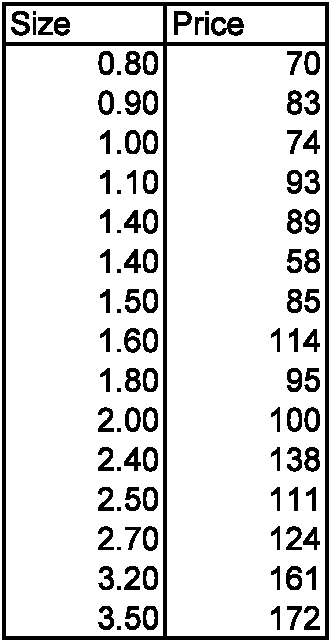
\includegraphics[width=1.3in]{figures/housedata}

\end{frame}

%%%%%%%%%%%%%%%%%%%%%%%%%%%%%%%%%%%%%%%%%%%%%%%%%%%%

\begin{frame}
\frametitle{Predicting house prices}

\vspace{2mm}
It is much more useful to look at a scatterplot \vspace{-10mm}
\begin{center}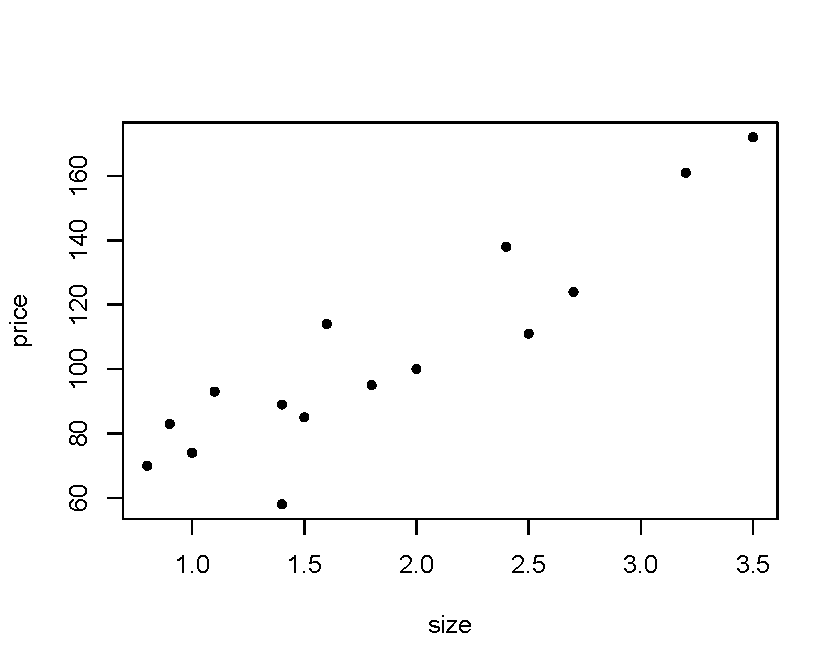
\includegraphics[scale=0.65]{figures/houseplot}\end{center}

\vspace{-5mm}
In other words, view the data as points in the $X
\times Y$ plane.
\end{frame}

%%%%%%%%%%%%%%%%%%%%%%%%%%%%%%%%%%%%%%%%%%%%%


%\begin{frame}
%\frametitle{Regression model} \vspace{-0.5cm}
%
%\bl $Y$ \bk= \rd response or outcome variable
%
%\bl $X$ \bk= \rd explanatory or input variables \bk
%
%\skoo 
%A  \bl linear \bk relationship is written
%\[
%Y = b_0 + b_1 X + e
%\]
%
%\end{frame}

%%%%%%%%%%%%%%%%%%%%%%%%%%%%%%%%%%%%%%%%%%%%%%%

\begin{frame}
\frametitle{Linear prediction}

\vspace{3mm}
There seems to be a linear relationship between 
price and size:\\ \vspace{3mm}
\centering \rd As size goes up, price goes up. \bk

\vspace{-6mm}
\begin{center}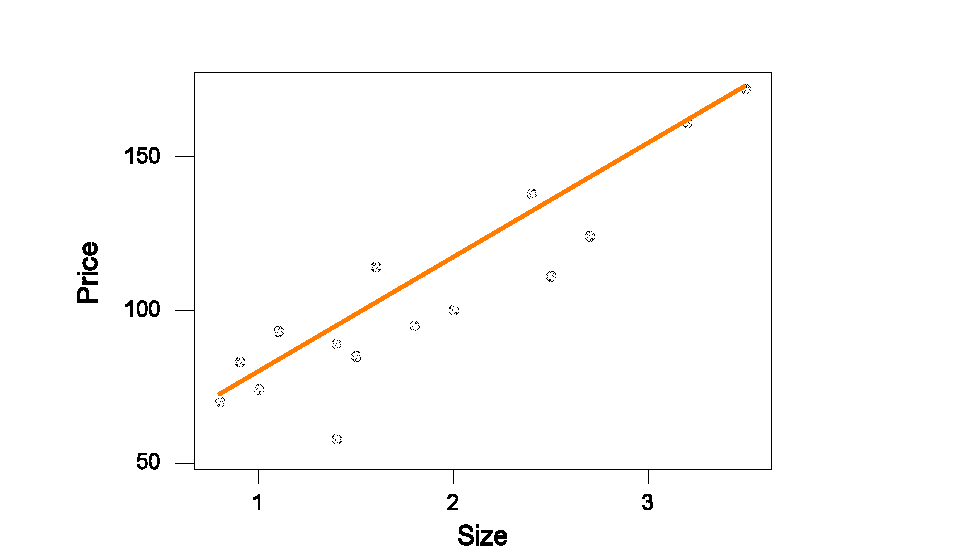
\includegraphics[scale=0.68]{figures/eyeball.pdf}\end{center}


\end{frame}
%%%%%%%%%%%%%%%%%%%%%%%%%%%%%%%%%%%%%%%%%%%%%%%%%

\begin{frame}
\frametitle{Linear prediction} \vspace{-0.5cm}

Recall that the equation of a line is: \vspace{3mm}
\[
				Y = b_0 + b_1 X
\]

\vspace{3mm}
Where  $b_0$ is the \lb{ \bf intercept} \bk and $b_1$ is the \lb{ \bf slope}\bk.

\sk
\sk
$\rightarrow$ The \lb{\bf intercept} value is in  units of $Y$ (\$1,000)\\ \sk
$\rightarrow$ The \lb{\bf slope} is in units of $Y$ {\it per} units of $X$ (\$1,000/1,000 sq ft)

\end{frame}

%%%%%%%%%%%%%%%%%%%%%%%%%%%%%%%%%%%%%%%%%%%%%%%%%

\begin{frame}
\frametitle{Linear prediction} \vspace{-0.5cm}

\begin{center}
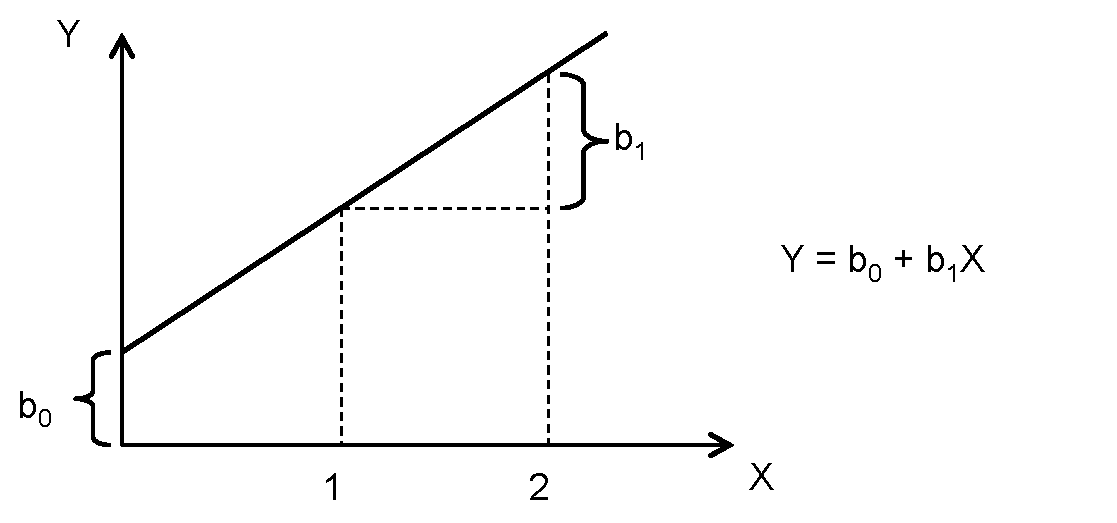
\includegraphics[scale=0.65]{figures/straightline}\\
\end{center}
\end{frame}

%%%%%%%%%%%%%%%%%%%%%%%%%%%%%%%%%%%%%%%%%%%%%%%%%%


%%%%%%%%%%%%%%%%%%%%%%%%%%%%%%%%%%%%%%%%%%%%%%%%


\begin{frame}
\frametitle{Linear prediction} \vspace{-0.5cm}

\begin{center} \rd
\bf{ \bf Q: How to find the ``best line''?}
\end{center} \bk

\sk
We desire a strategy for estimating the slope and intercept parameters
in the model
$\hat{Y} = b_0 + b_1 X$

\sk
A reasonable way to fit a line is to minimize the amount by which the
\bl fitted value \bk differs from the actual value. 

\sk	This amount is called the \bl residual. \bk 

\end{frame}


%%%%%%%%%%%%%%%%%%%%%%%%%%%%%%%%%%%%%%%%%%%%%


\begin{frame}
\frametitle{Linear prediction}

What is the ``fitted value''?

\vskip 0.5cm
\hskip 1.5cm 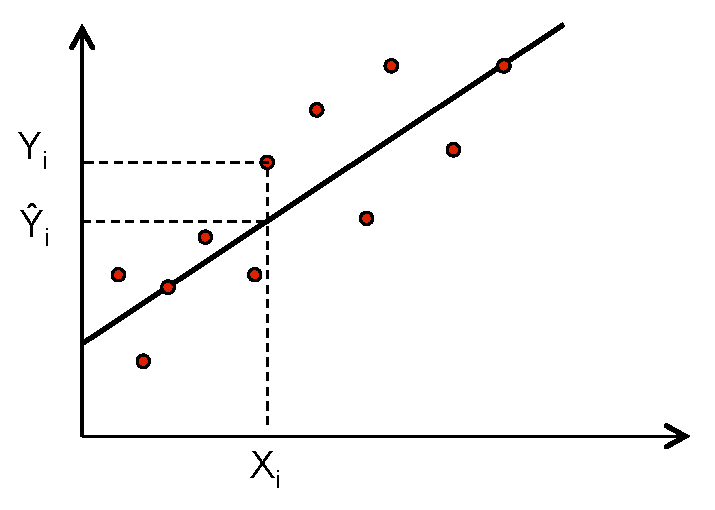
\includegraphics[scale=0.65]{figures/fittedval}

The dots are the observed values and the line represents our fitted
values given by \bl
$
\hat{Y}_i = b_0 + b_1 X_1
$ \bk.

\end{frame}
%%%%%%%%%%%%%%%%%%%%%%%%%%%%%%%%%%%%%%%%%%%%%%%

\begin{frame}
\frametitle{Linear prediction}

What is the ``residual''' for the $i$th observation?

\vskip .5cm
~~~~~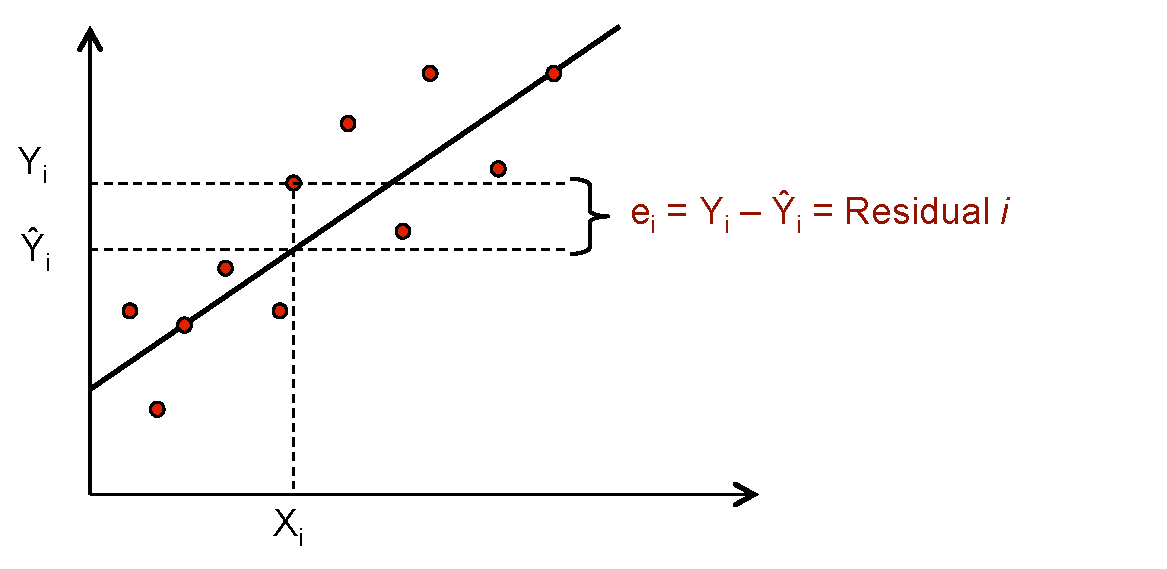
\includegraphics[scale=0.6]{figures/residual}

We can write \bl
$
Y_i = \hat{Y}_i + (Y_i -\hat{Y}_i) = \hat{Y}_i + e_i
$ \bk.

\end{frame}

%%%%%%%%%%%%%%%%%%%%%%%%%%%%%%%%%%%%%%%%%%%%%%%%

\begin{frame}
\frametitle{Least squares} \vspace{-0.5cm}

\sk
\sk
Ideally, we want to minimize the size of all residuals: \vspace{2mm}
\bi
\p If they were all zero we would have a perfect line.
\p Trade-off between moving closer to some points and at the same time moving away from other points.
\ib

\pause

\sk
\dg{\underline{The line fitting process}}: \vspace{2mm}
\bi
\p Minimize the ``total'' of residuals to get best fit.
\ib

\vspace{-3mm}

\pause
\begin{center}\bl \large
Least Squares chooses $b_0$ and $b_1$ to minimize \rd $\sum_{i=1}^N e^2_i$\bk
\end{center}
$$
{\rd \sum_{i=1}^N e^2_i} = e^2_1 + e^2_2 + \dots + e^2_N = (Y_1 - \hat{Y}_1)^2 +(Y_2 - \hat{Y}_2)^2+\dots+(Y_N - \hat{Y}_N)^2
 $$


\end{frame}
%%%%%%%%%%%%%%%%%%%%%%%%%%%%%%%%%%%%%%%%%%%%%%%%
%
%
%\begin{frame}
%\frametitle{Least Squares} 
%
%\hskip 1cm \includegraphics[width=3.25in]{negpos}
%
%{\small Choose the line to minimize the sum of the squares of the
%residuals,}
%\[
%\sum_{i=1}^n e^2_i = \sum_{i=1}^n (Y_i - \hat{Y}_i)^2 
%= \sum_{i=1}^n (Y_i - [b_0 + b_1 X_i])^2
%\]
%
%\end{frame}
%
%%%%%%%%%%%%%%%%%%%%%%%%%%%%%%%%%%%%%%%%%%%%%%




%%%%%%%%%%%%%%%%%%%%%%%%%%%%%%%%%%%%%%%%%%%%%%
%
%
%\begin{frame}
%\frametitle{Eyeball vs. LS Residuals} 
%\begin{itemize}
%\item {\color{red}eyeball: $b_0=35$, $b_1=40$}
%\item {\color{blue}LS: $b_0 =38.88$, $b_1=35.39$} 
%\end{itemize}
%\begin{center}
%%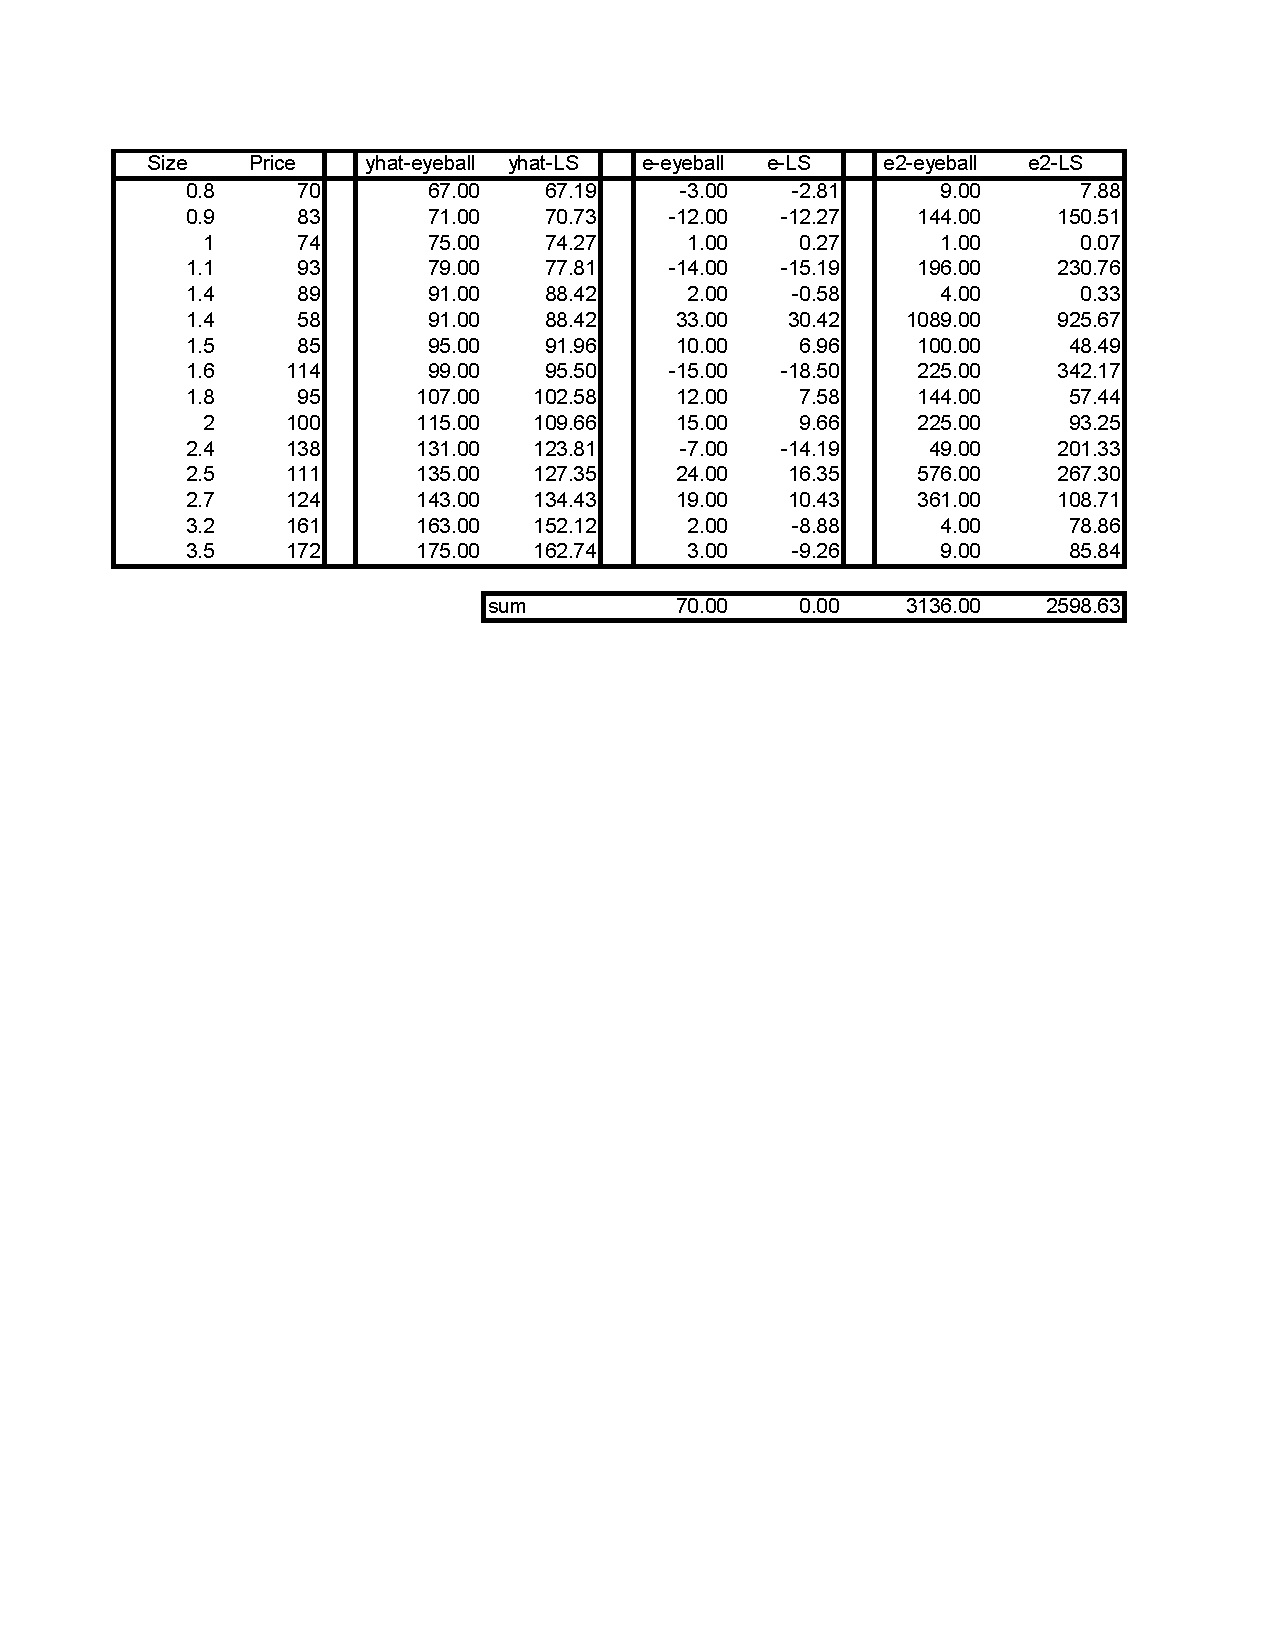
\includegraphics[width=4.5in]{housedata-table}
%\includegraphics[width=4.5in]{newOutput}
%\end{center}
%
%\end{frame}
%%%%%%%%%%%%%%%%%%%%%%%%%%%%%%%%%%%%%%%%%%%%%%


%\begin{frame}
%\frametitle{Least squares -- {\tt R} output} 
%
%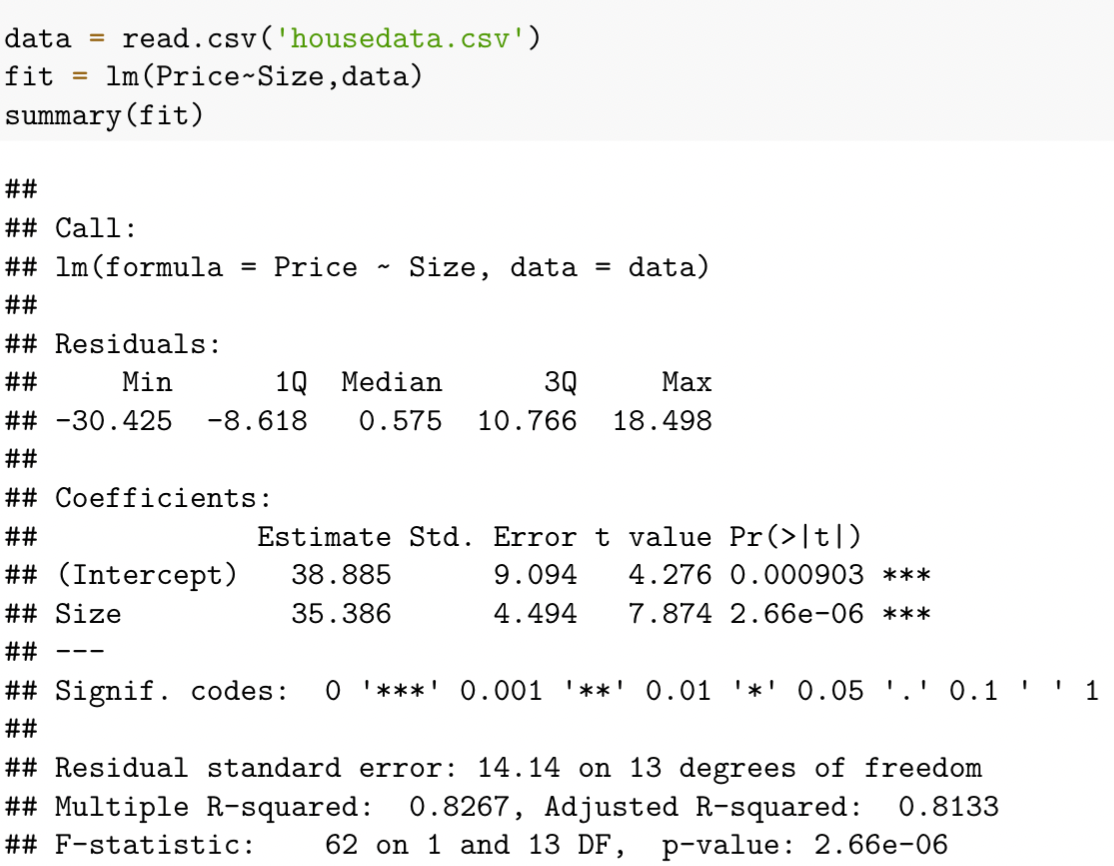
\includegraphics[scale=0.50]{figures/pred1}
%
%\end{frame}




\begin{frame}
\frametitle{Example 2: Offensive performance in baseball} 


{\lb{Problems}}:
\bi
\item Evaluate/compare traditional measures of offensive performance
\item Help evaluate the worth of a player
\ib

\sk
\sk

{\lb {Solutions}}:
\bi
\item Compare {\bo{ \it prediction rules}} that forecast runs as a function of either \bo{AVG} (batting average), \bo{SLG} (slugging percentage -- {\small total bases divided by at bats}) or \bo{OBP} (on base percentage)
\ib


\end{frame}




\begin{frame}
\frametitle{Example 2: Offensive performance in baseball} 

\begin{center}

\includegraphics[width=2in]{figures/Moneyball.pdf}
\end{center}
\end{frame}

%%%%%%%%%%%%%%%%%%%%%%%%%%%%%%%%%%%%%%%%
\begin{frame}
\frametitle{Baseball data -- using AVG} 

\sk
Each observation corresponds to a team in MLB. Each quantity is the average over a season. 

\vspace{-3mm}
\begin{center}
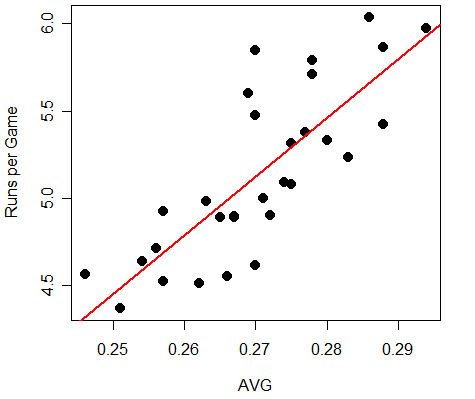
\includegraphics[scale=0.42]{figures/AvgR.png}	
\end{center}

\vspace{-5.8mm}
$Y=$ runs per game; $X=$ AVG (average)


LS fit: {\color{red} Runs/Game = -3.93 + 33.57 AVG}
\end{frame}

\begin{frame}
\frametitle{Baseball data -- using AVG} 

\vspace{-5.8mm}
\begin{center}
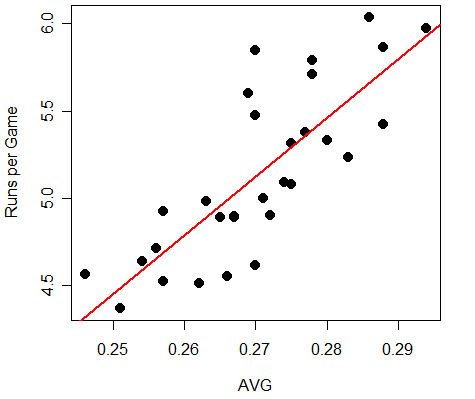
\includegraphics[scale=0.42]{figures/AvgR.png}	
\end{center}

\vspace{-5.8mm}
$Y=$ runs per game; $X=$ AVG (average)

\vspace{1mm}
LS fit: {\color{red} Runs/Game = -3.93 + 33.57 AVG}
\end{frame}

%%%%%%%%%%%%%%%%%%%%%%%%%%%%%%%%%%%%%%
\begin{frame}
\frametitle{Baseball data -- using SLG} 

\vspace{-5.8mm}
\begin{center}
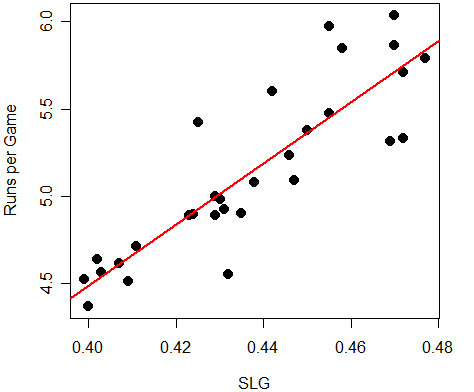
\includegraphics[scale=0.42]{figures/SlgR.png}
\end{center}

\vspace{-5.8mm}
$Y=$ runs per game; $X=$ SLG (slugging percentage)

\vspace{1mm}
LS fit: {\color{red} Runs/Game = -2.52 + 17.54 SLG}
\end{frame}


%%%%%%%%%%%%%%%%%%%%%%%%%%%%%%%%%%%%%%%%
\begin{frame}
\frametitle{Baseball data -- using OBP} 

\vspace{-5.8mm}
\begin{center}
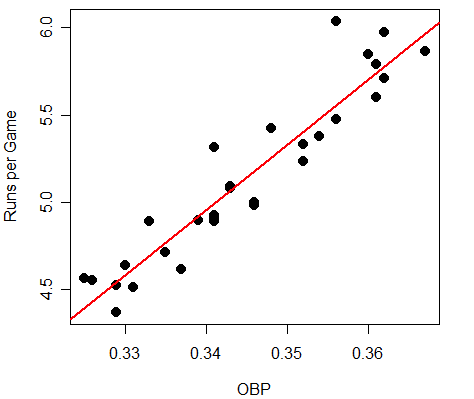
\includegraphics[scale=0.42]{figures/OBPR.png}
\end{center}

\vspace{-5.8mm}
$Y=$ runs per game; $X=$ OBP (on base percentage)

\vspace{1mm}
LS fit: {\color{red} Runs/Game = -7.78 + 37.46 OBP}
\end{frame}


%%%%%%%%%%%%%%%%%%%%%%%%%%%%%%%%%%%%%%
\begin{frame}
\frametitle{Baseball data}
\bi
\item {\bo{ What is the best prediction rule?}}
\item Let's compare the predictive ability of each model using the average squared error
\ib

$$
\sqrt{\frac{1}{N}\sum_{i=1}^N{e_i^2}}  = \left(\frac{\sum_{i=1}^N{\left(\widehat{\text{Runs}_i} - \text{Runs}_i \right)^2}}{N}\right)^{\frac{1}{2}}
$$
\end{frame}
%%%%%%%%%%%%%%%%%%%%%%%%%%%%%%%%%%%%%%%

\begin{frame}
\frametitle{Place your money on OBP!}
\begin{center}
{\Large
\begin{tabular}{cc}
\hline
& Root Mean Squared Error \\
\hline 
AVG & 0.29 \\
SLG & 0.23 \\
{\bo{ OBP}} & {\bo{ 0.16}} \\
\hline
\end{tabular}
}
\end{center}
\end{frame}
%%%%%%%%%%%%%%%%%%%%%%%%%%%%%%%%%%


%%%%%%%%%%%%%%%%%%%%%%%%%%%%%%%%%%%%%%%%%%%%%%%%%
\begin{frame}
\frametitle{More on least squares}
Remember how we get the slope (\bo{$b_1$}) and intercept (\bo{$b_0$}).  \dg{We minimize the sum of squared prediction errors}.

\sk
The formulas for $b_0$ and $b_1$ that minimize the least squares criterion are:
{\lb{ \Large
$$
b_1 = r_{xy} \times \frac{s_y}{s_x}  \quad \mbox \quad b_0 = \bar{Y} - b_1 \bar{X}
$$
}}
where,

\begin{itemize}
\item $\bar{X}$ and $\bar{Y}$ are the sample mean of $X$ and $Y$
\item $\text{corr}(x,y) = r_{xy}$ is the sample correlation
\item $s_x$ and $s_y$ are the sample standard deviation of $X$ and $Y$
\end{itemize}



\end{frame}


\begin{frame}
\frametitle{What are these numbers in the formula?}

\begin{itemize}
\item {\color{lightblue} Sample Mean:}  measure of \bo{centrality}
$$
\bar{Y} = \frac{1}{n}\sum^{n}_{i=1}{Y_i }
$$ 

\item {\color{lightblue} Sample Variance}: measure of \bo{spread} 
$$
s^2_y= \frac{1}{n-1}\sum^{n}_{i=1}{\left(Y_i - \bar{Y}\right)^2 }
$$ 

\item {\color{lightblue} Sample Standard Deviation}:
$$
s_y= \sqrt{s^2_y} 
$$ 


\end{itemize} 
\end{frame}


\begin{frame}
\frametitle{Visual: standard deviation}

\vspace{-0.5cm}
$$
s^2_y =  \frac{1}{n-1}\sum^{n}_{i=1}{\left(Y_i - \bar{Y}\right)^2 }
$$

\vspace{-0.4cm}

\begin{center}
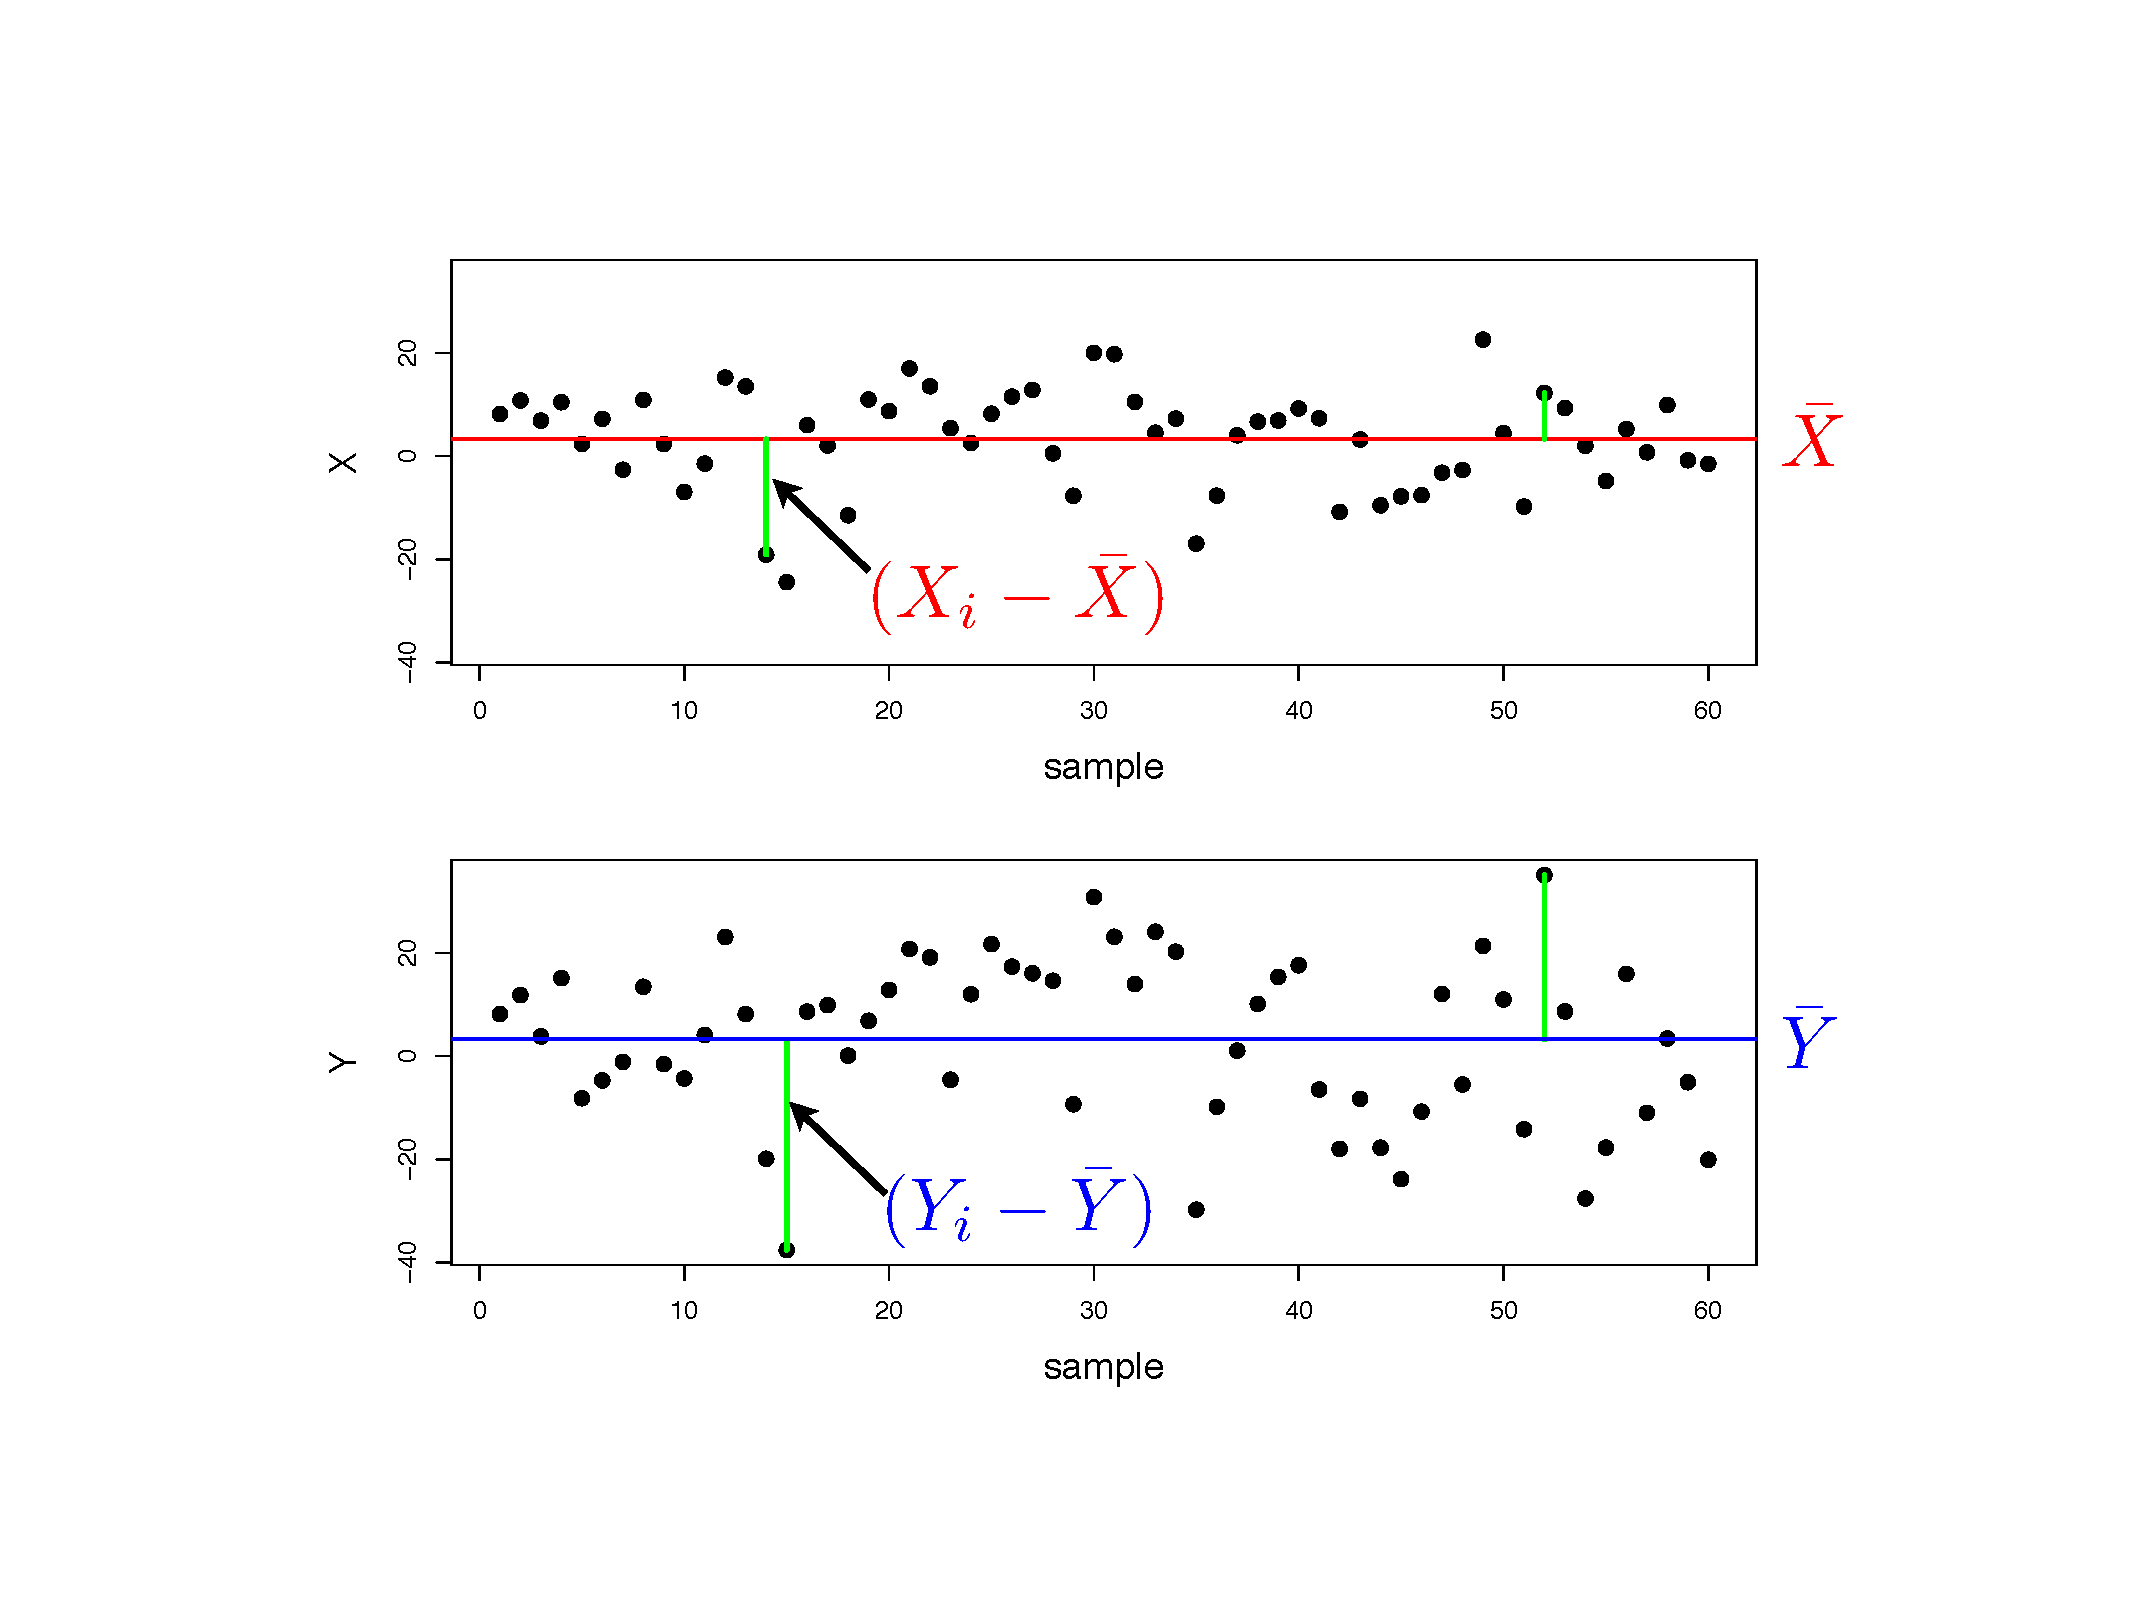
\includegraphics[width=3.4in]{figures/stdevpicnew.pdf}
\end{center}

\vspace{-1cm}

$$
{\color{red} s_x = 9.7} \quad \quad {\color{blue} s_y = 15.98}
$$

\end{frame}


\begin{frame}
\frametitle{Visual: Covariance} 
{\scriptsize
Measure the {\color{burntorange} \bf direction} and {\color{burntorange} \bf strength} of the linear relationship between $Y$ and $X$ 

$$
\text{cov}(Y,X) = \frac{\sum_{i=1}^n{(Y_i - \bar{Y})(X_i - \bar{X})}}{n-1}
$$
}

\vspace{-0.5cm}

\hspace{-0.5cm}
\begin{minipage}{2.65in}
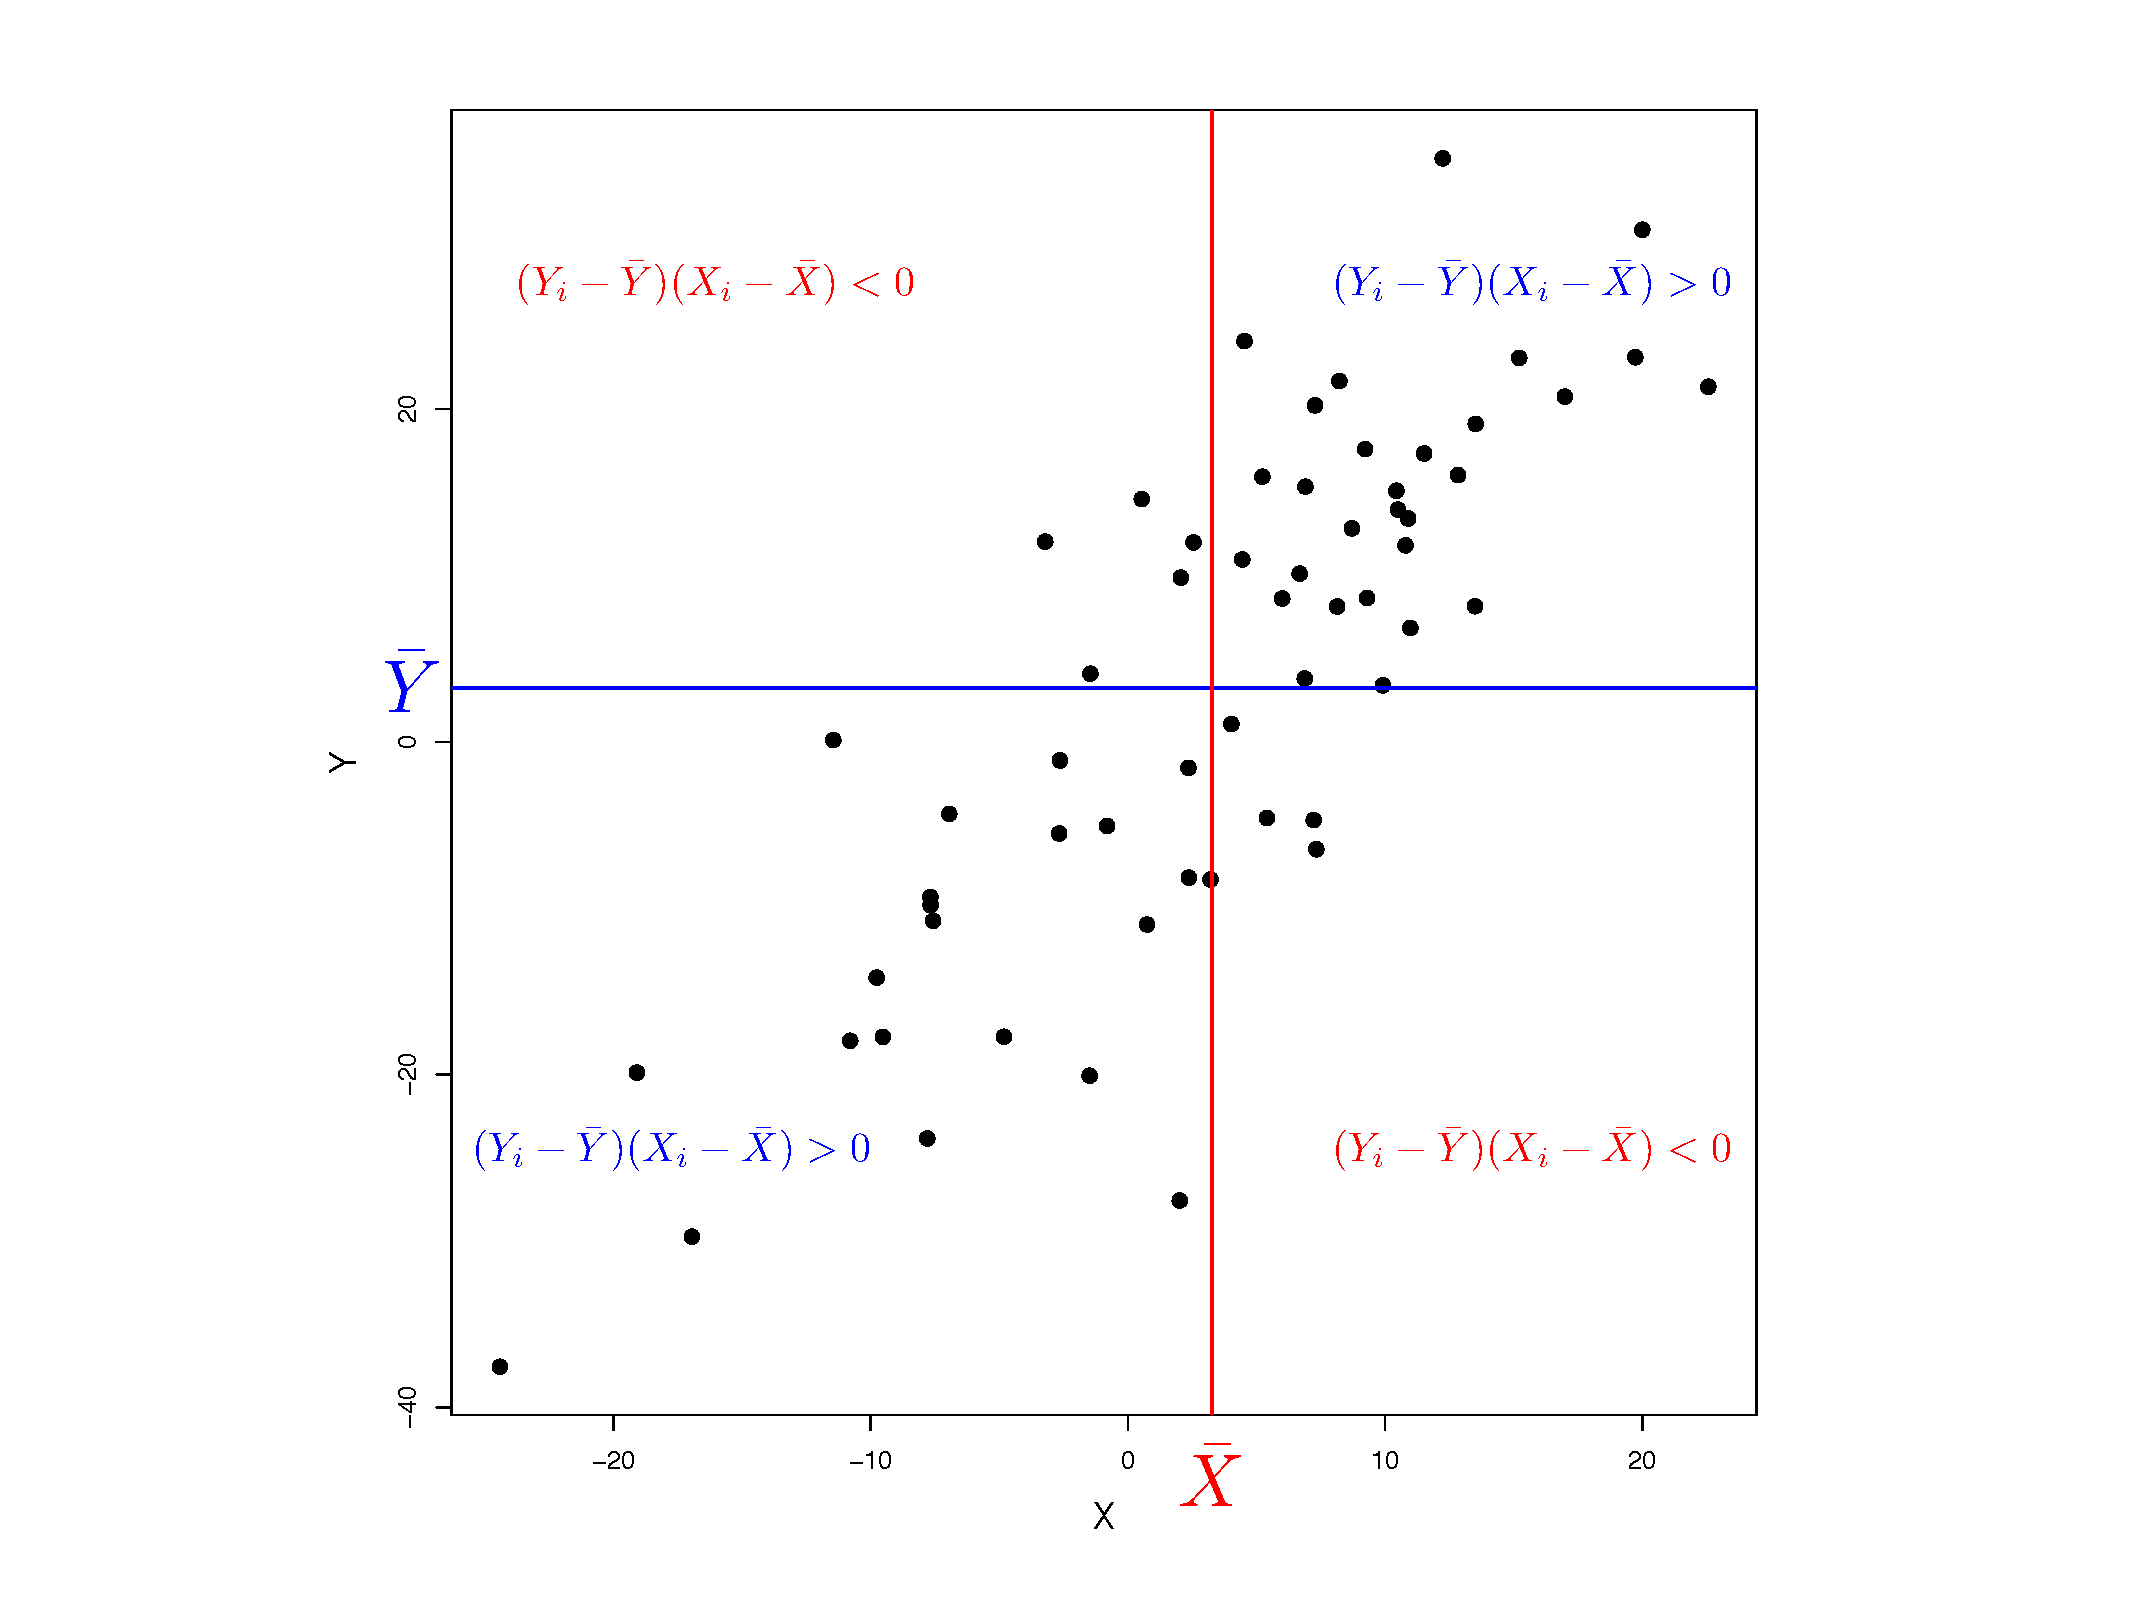
\includegraphics[width=2.7in]{figures/cor-pic.pdf}
\end{minipage}
\begin{minipage}{1.65in}
\begin{itemize}
\item $s_y   = 15.98$, $s_x = 9.7$
\item $\text{cov}(X,Y) = 125.9$
\end{itemize}

\vspace{3mm}
\hspace*{3.5mm} \small \lb{How do we interpret that?}
\end{minipage}


\end{frame}

\begin{frame}
\frametitle{A standardized measure: Correlation}

\bo{Correlation} is the standardized covariance: \sk
\[
\mr{corr}(X,Y) = \frac{\mr{cov}(X,Y)}{\sqrt{s^2_x s^2_y}} = \frac{\mr{cov}(X,Y)}{s_x s_y} 
\]

\sk
The correlation  is scale invariant and the units of measurement don't
matter: \bl
It is always true that $-1 \leq \mr{corr}(X,Y) \leq 1$. \bk

\sk
\sk
This gives the direction (\color{red} negative \bk or \color{green} positive\bk) and strength
($0\rightarrow 1$) \\of the \bl linear \bk relationship between $X$ and
$Y$.

\end{frame}


\begin{frame}
\frametitle{Correlation} 

\vspace{-1mm}
$$
\text{corr}(Y,X) = \frac{\mr{cov}(X,Y)}{\sqrt{s^2_x s^2_y}} = \frac{\mr{cov}(X,Y)}{s_x s_y} =\frac{125.9}{15.98 \times 9.7} = 0.812
$$

\vspace{-2mm}
\hspace*{20mm}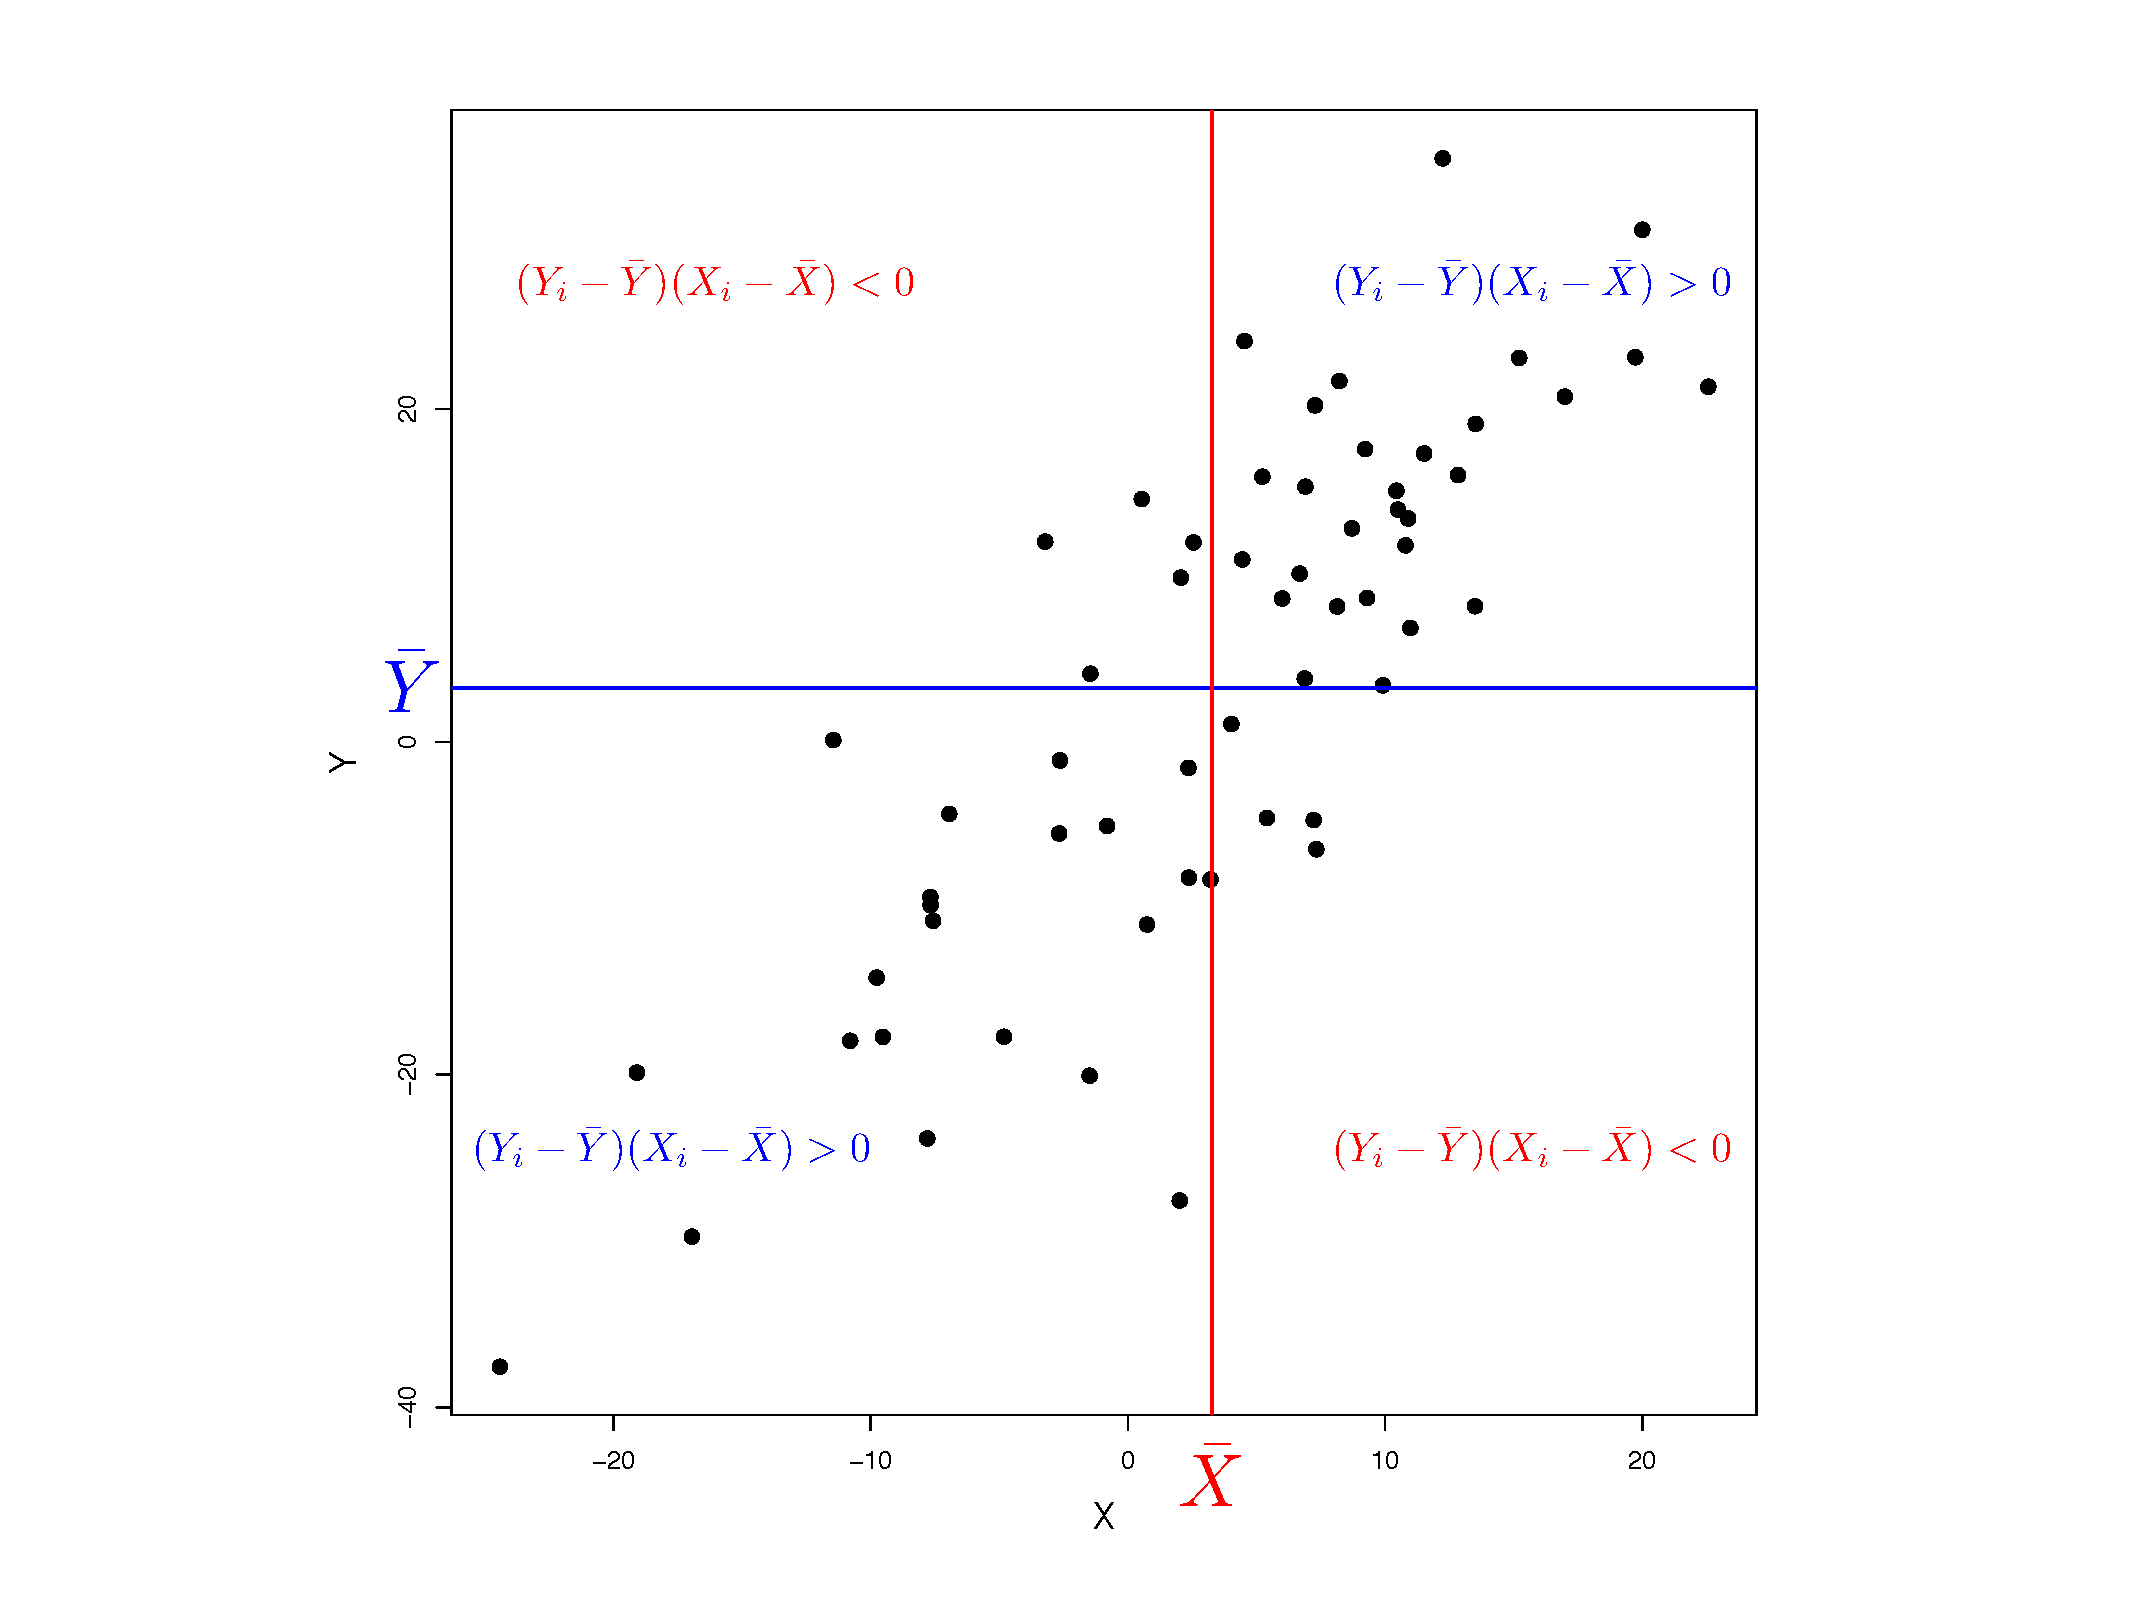
\includegraphics[width=2.5in]{figures/cor-pic.pdf}


\end{frame}

%%%%%%%%%%%%%%%%%%%%%%%%%%%%%%%%%%%%%%%%%%%%%%%
\begin{frame}
\frametitle{Correlation}

\centering 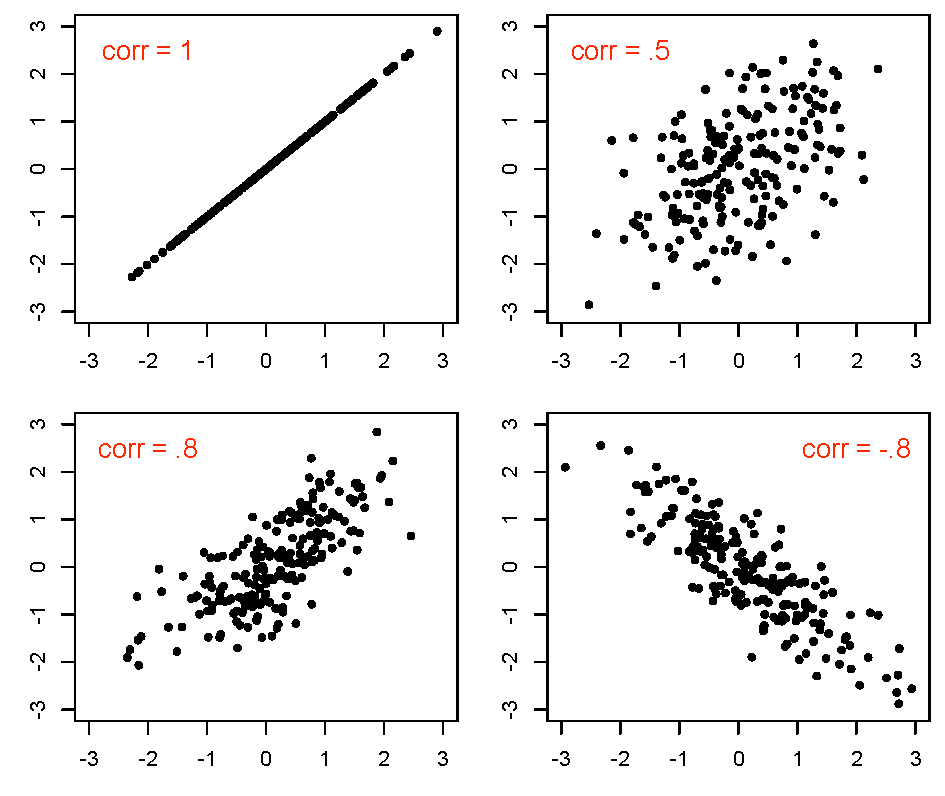
\includegraphics[width=3.7in]{figures/corr}

\end{frame}
%%%%%%%%%%%%%%%%%%%%%%%%%%%%%%%%%%%%%%%%%%%%%%%

\begin{frame}
\frametitle{Correlation}

Only measures \rd linear \bk relationships: \\ \vspace{3mm} corr$(X,Y) =0 $ does not
mean the variables are not related!

\begin{center}
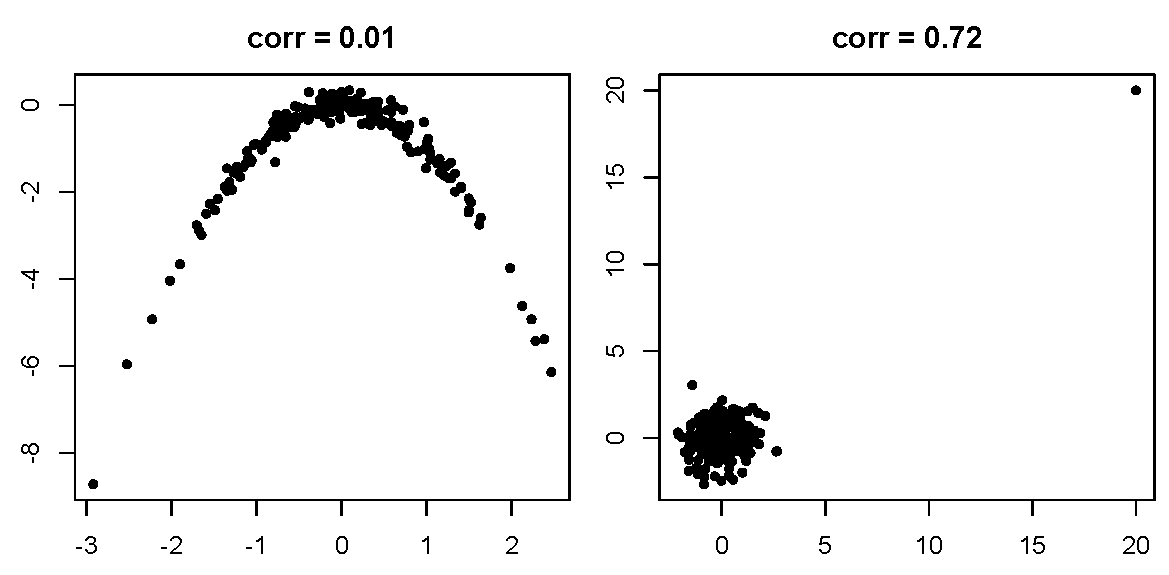
\includegraphics[width=4in]{figures/strangecor}
\end{center}
Also be careful with influential observations.  Check out {\tt cor()} in {\tt R}.

\end{frame}
%%%%%%%%%%%%%%%%%%%%%%%%%%%%%%%%%%%%%%%%%%%%%
%\begin{frame}
%\frametitle{Back to least squares}
%
%{\color{lightblue} Intercept:}
%$$
%b_0 = \bar{Y} -b_1 \bar{X} \Rightarrow \bar{Y} = b_0 + b_1 \bar{X} 
%$$
%
%
%The point $(\bar{X},\bar{Y})$ is on the regression line! \\ \vspace{2mm}
%Least squares finds the point of means and rotates the line through that point until getting the ``right'' slope
%
%\vspace{2mm}
%{\color{lightblue}Slope:}
%\begin{equation*}
%\begin{split}
%b_1 = \text{corr}(X,Y) \times \frac{s_Y}{s_X} =&  \frac{\sum_{i=1}^n (X_i - \bar{X})(Y_i -
%  \bar{Y})}{\sum_{i=1}^n (X_i - \bar{X})^2} \\
%   =& \frac{\text{cov}(X,Y)}{\text{var}(X)}	
%\end{split}
%\end{equation*} \vspace{2mm}
%
%
%So, the right slope is the {\color{burntorange} \bf correlation coefficient} times a {\color{burntorange} \bf scaling factor} that ensures the proper units for $b_1$
%
%\end{frame}
%%%%%%%%%%%%%%%%%%%%%%%%%%%%%%%%%%%%%%%%%%%%%%%

\begin{frame}
\frametitle{More on least squares}

From now on,  terms \bl``fitted values''  ($\hat{Y}_i$) \bk
and \bl ``residuals'' ($e_i$) \bk refer to those obtained 
from the least squares line. 

\sk

\sk The fitted values and residuals have some \bo{special properties}.
Let's look at the housing data analysis to figure out 
what these properties are...


\end{frame}
%%%%%%%%%%%%%%%%%%%%%%%%%%%%%%%%%%%%%%%%%%%%%%%%%

\begin{frame}
\frametitle{The fitted values and X}

\hspace*{-3mm}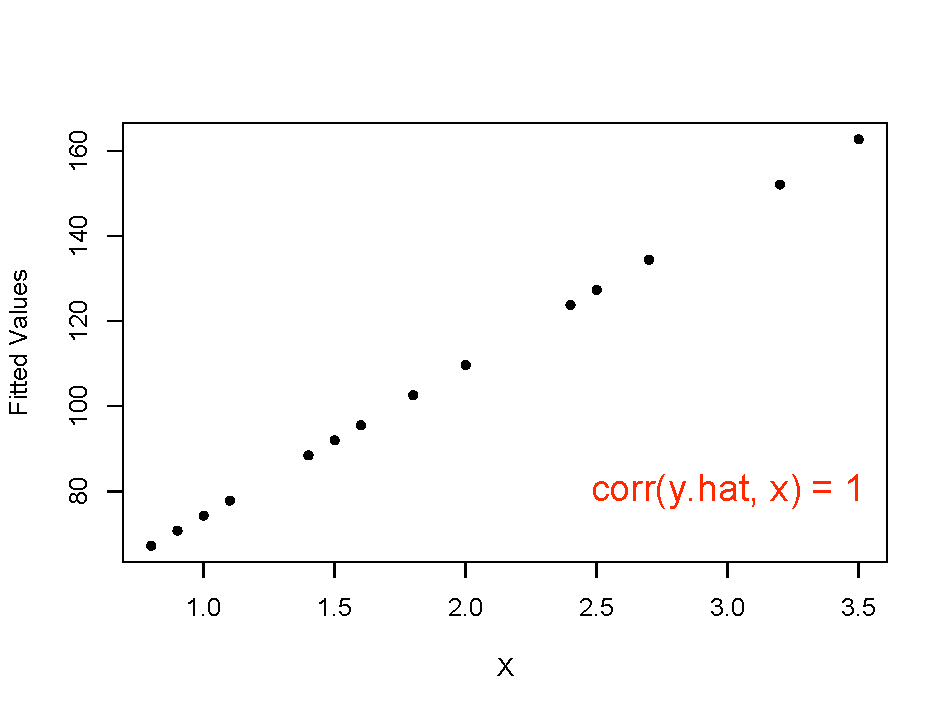
\includegraphics[width=4.3in]{figures/fittedVx}

\end{frame}


\begin{frame}
\frametitle{The residuals and X}

\hspace*{-3mm}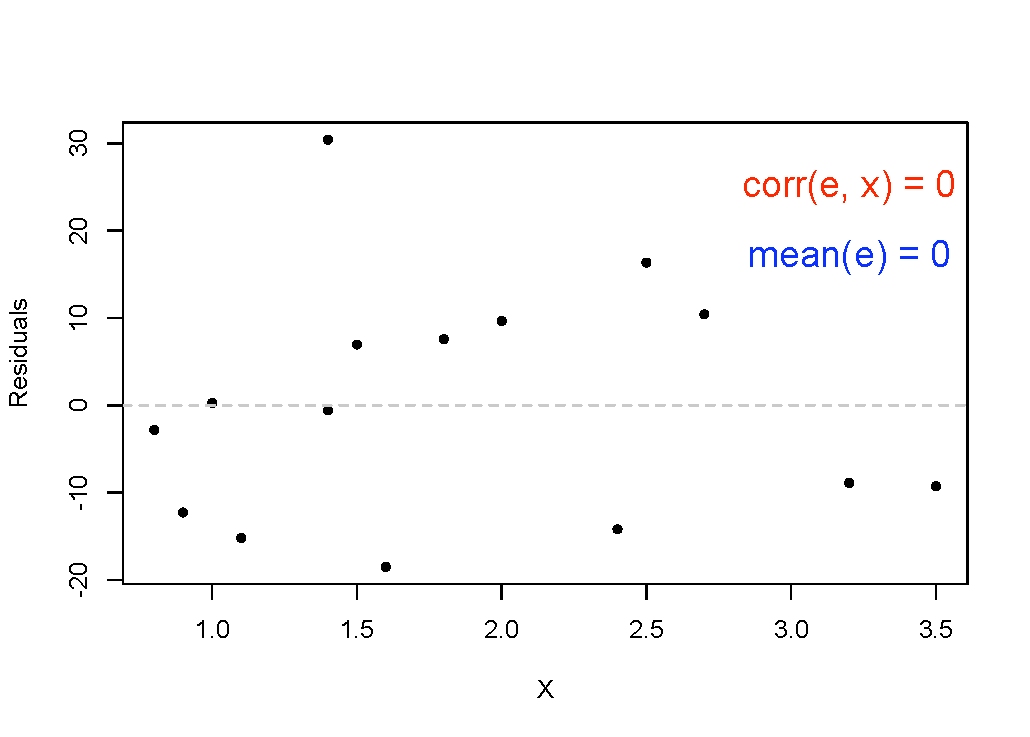
\includegraphics[width=4.3in]{figures/eVx}

\end{frame}
%%%%%%%%%%%%%%%%%%%%%%%%%%%%%%%%%%%%%%%%%%%%%%%%%

\begin{frame}
\frametitle{Why?}

\sk
What is the intuition for the relationship between $\hat{Y}$ and $e$
and $X$? Lets consider some \rd``crazy''\bk alternative line:
\vskip -.75cm
\hspace*{-3mm}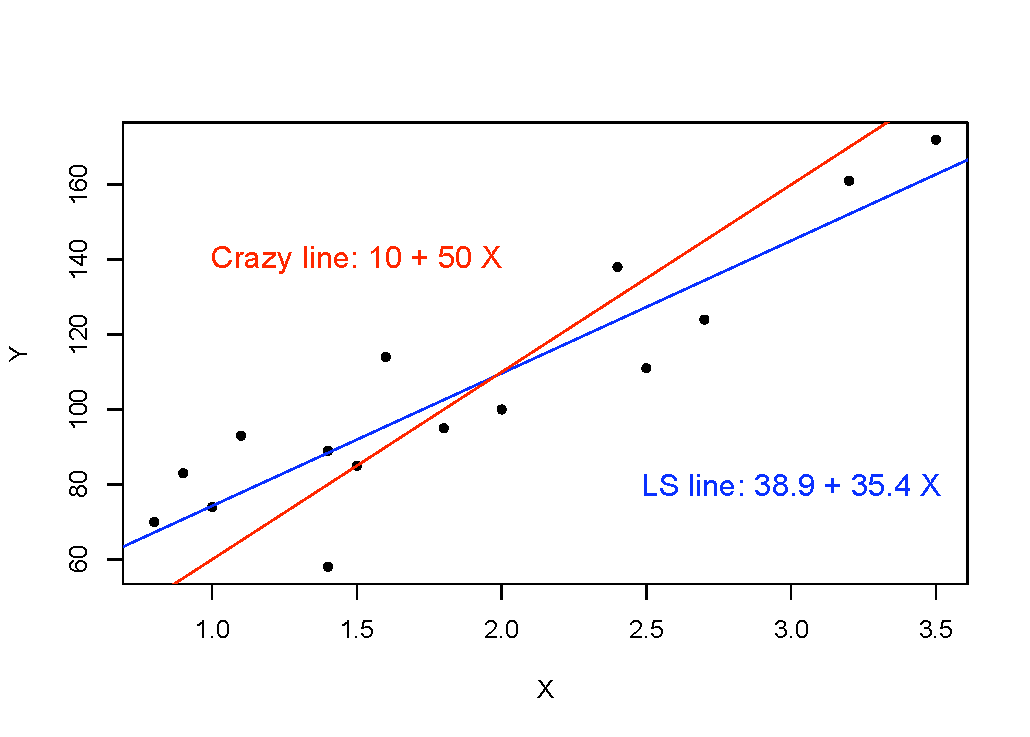
\includegraphics[width=4.3in]{figures/crazyline}

\end{frame}
%%%%%%%%%%%%%%%%%%%%%%%%%%%%%%%%%%%%%%%%%%%%%%%%%%%
\begin{frame}
\frametitle{Fitted values and residuals}

\bl This is a bad fit!  \bk We are underestimating the value of small houses
and overestimating the value of big houses.
\vskip -.6cm
~~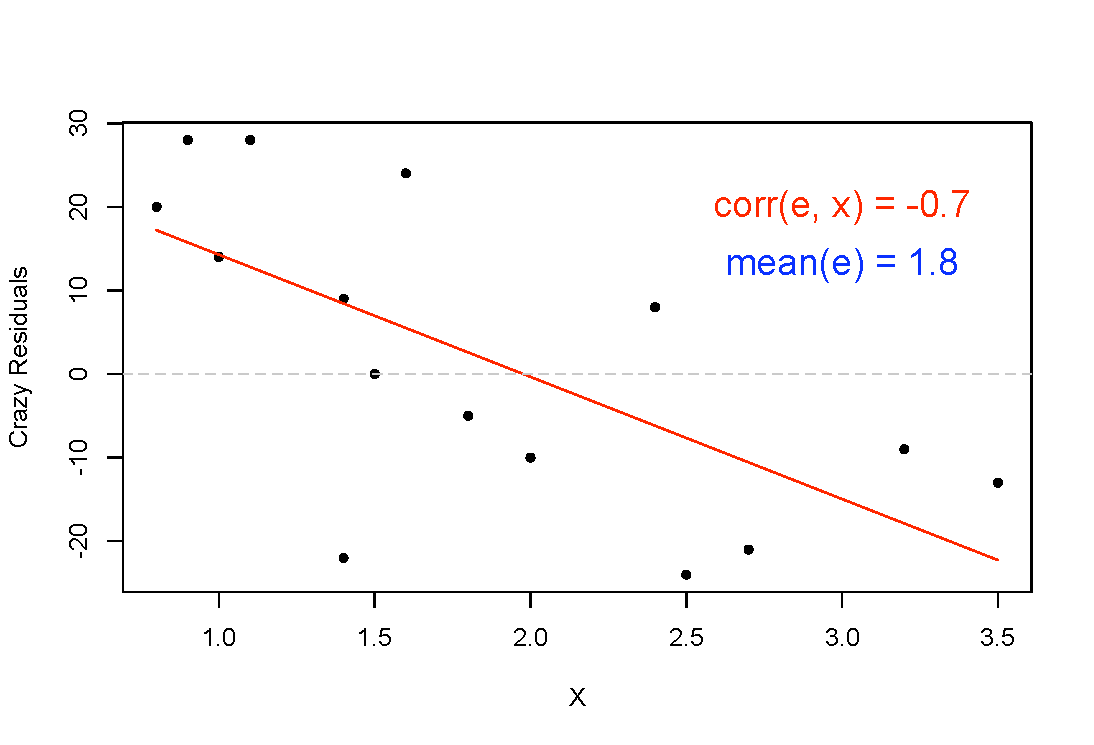
\includegraphics[width=4in]{figures/crazyresid}\\
\vskip -.4cm
Clearly, we have left some predictive ability on the table!

\end{frame}
%%%%%%%%%%%%%%%%%%%%%%%%%%%%%%%%%%%%%%%%%%%%%%%%%%%

\begin{frame}
\frametitle{Fitted values and residuals}

As long as the correlation between $e$ and $X$ is non-zero, we 
could always adjust our prediction rule to do better.

\sk\sk
We need to exploit all of the predictive power in the 
$X$ values and put this into $\hat{Y}$,  leaving no ``$Xness$'' in the
residuals. 

\sk\sk
\bl {\bf In summary}: $Y = \hat{Y} + e$ where:\bk \vspace{2mm}
\bi
\p $\hat{Y}$ is ``made from $X$''; \rd corr($X,\hat{Y}$) = 1.\bk
\p $e$ is unrelated to $X$; \rd corr($X,e$) = 0.\bk
\ib

\end{frame}


%\begin{frame}
%\frametitle{Decomposing the variance}
%\rd {\bf Q:} How well does the least squares line explain variation in $Y$?
%\bk
%
%\sk
%Remember that $Y = \hat{Y} + e $
%
%\sk Since $\hat{Y}$ and $e$ are uncorrelated, i.e. $\mr{corr}(\hat{Y},
%e) = 0$, 
%\begin{equation*}
%	\begin{split}
%\mr{var}(Y) = \mr{var}(\hat{Y} + e) =& {\color{blue}\mr{var}(\hat{Y})} +
%{\color{red}\mr{var}(e)} \\ 
%\frac{\sum_{i=1}^n (Y_i - \bar{Y})^2}{n-1} =& {\color{blue}\frac{\sum_{i=1}^n (\hat{Y}_i - \bar{\hat{Y}})^2}{n-1}} + {\color{red}\frac{\sum_{i=1}^n (e_i-\bar{e})^2 }{n-1}} 		
%	\end{split}
%\end{equation*}
%
%
%Given that $\bar{e} = 0$, and $\bar{\hat{Y}} = \bar{Y}$ (why?) we get to: 
%
%\vspace{-2mm}
%\sk
%\begin{tcolorbox}
%\[
%\sum_{i=1}^n (Y_i - \bar{Y})^2 = 
%\sum_{i=1}^n (\hat{Y}_i - \bar{Y})^2 + \sum_{i=1}^n e_i^2 
%\]	
%\end{tcolorbox}
%
%\end{frame}
%
%\begin{frame}
%\frametitle{Decomposing the variance} 
%
%
%~~~~
%\hspace*{-4mm}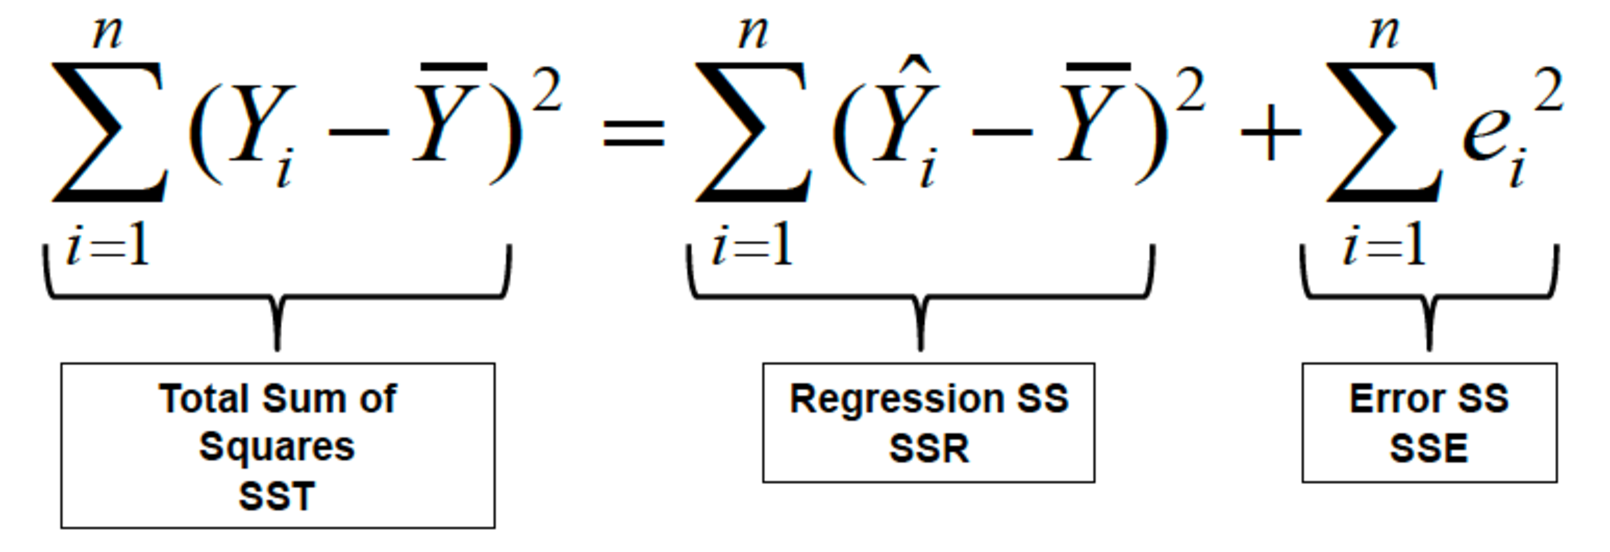
\includegraphics[width=3.8in]{figures/anovaeqns}
%
%\sk 
%SSR: Variation in $Y$ explained by the regression line.\\
%SSE: Variation in $Y$ that is left unexplained.
%
%\sk\pause
%\begin{center} \large
%SSR = SST \rd $\Rightarrow$ \bk perfect fit.
%\end{center}
%
%\it Be careful of similar acronyms; e.g. SSR for ``residual'' SS.
%\end{frame}
%%%%%%%%%%%%%%%%%%%%%%%%%%%%%%%%%%%%%%%%%%%%%%%%
%
%%\begin{frame}
%%\frametitle{Decomposing the Variance} 
%%\vspace{-0.7cm}
%%
%%\begin{eqnarray*}
%%(Y_i  {\color{red}-\bar{Y}}) &=& \hat{Y}_i + e_i  {\color{red}-\bar{Y}} \\
%%&=& (\hat{Y}_i - \bar{Y}) + e_i
%%\end{eqnarray*}
%%
%%\vspace{-0.5cm}
%%\begin{center}
%%\includegraphics[width=4.3in]{anova}
%%\end{center}
%%
%%\end{frame}
%%%%%%%%%%%%%%%%%%%%%%%%%%%%%%%%%%%%%%%%%%%%%%%%%%
%
%\begin{frame}
%\frametitle{A goodness of fit measure: $R^2$} 
%
%The \rd coefficient of determination\bk, denoted by \rd$R^2$\bk, \\
%measures goodness of fit: 
%\sk{\large \bl
%\[
%R^2 = \frac{\mr{SSR}}{\mr{SST}} = 1- \frac{\mr{SSE}}{\mr{SST}}
%\]}
%\bi
%\p $0 < R^2 < 1$.
%\p The closer $R^2$ is to 1, the better the fit.
%\ib
%
%\end{frame}
%
%
%\begin{frame}
%\frametitle{Back to baseball}
%
%Three very similar, related ways to look at a simple linear regression... with only one $X$ variable, life is easy!  
%
%\sk
%\sk
%\begin{center}
%\Large
%\begin{tabular}{|l|c|c|c|}
%\hline
%&$R^2$&corr& SSE \\
%\hline
%{\color{burntorange}OBP}& {\color{burntorange}0.88}& {\color{burntorange}0.94}& {\color{burntorange}0.79}  \\
%SLG& 0.76&0.87 & 1.64 \\
%AVG& 0.63 & 0.79&2.49  \\
%\hline
%\end{tabular}
%\end{center}
%\end{frame}
%
%\begin{frame}
%\sk\sk
%	\dg{\bf Prediction and regression + probability }
%\end{frame}
%
%
%\begin{frame}
%\frametitle{Prediction and the modeling goal}
%
%\large
%A prediction rule is any function where you input $X$ and it outputs
%$\hat{Y}$ as a predicted  response at $X$.
%
%\sk \sk
%The least squares line is a prediction rule:
%\[
%\hat{Y} = f(X) = b_0 + b_1 X
%\]
%
%\end{frame}
%%%%%%%%%%%%%%%%%%%%%%%%%%%%%%%%%%%%%%%%%%%%%%%%%%
%
%\begin{frame}
%\frametitle{Prediction and the modeling goal}
%
%$\hat{Y}$ is not going to be a perfect prediction.
%
%\sk
%We need to devise a notion of {\bf\bl forecast accuracy\bl}.
%
%\sk ~~~~~
%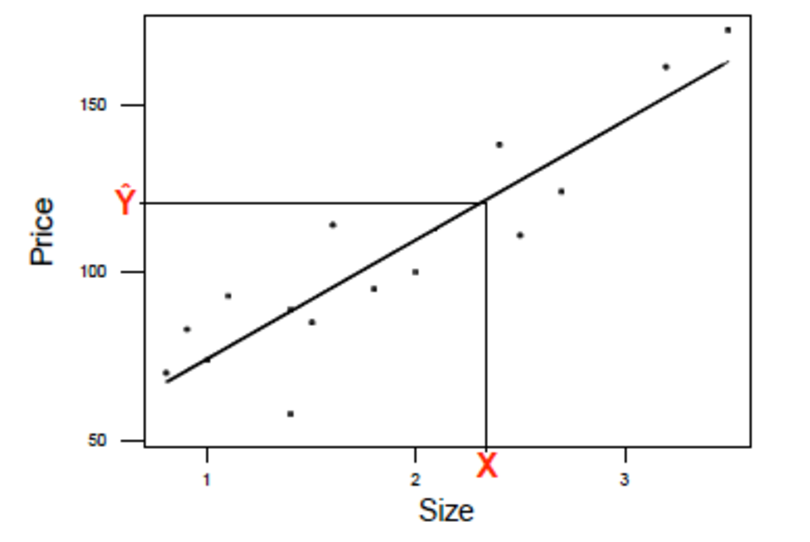
\includegraphics[width=3.3in]{figures/xypred}
%
%\end{frame}
%%%%%%%%%%%%%%%%%%%%%%%%%%%%%%%%%%%%%%%%%%%%%%%%
%
%\begin{frame}
%\frametitle{Prediction and the modeling goal}
%
%There are two things that we want to know:\vspace{2mm}
%\bi
%\p What value of $Y$ can we expect for a given $X$?
%\p How \underline{sure} are we about this forecast? Or how different could $Y$ be
%from what we expect?
%\ib
%
%\sk
%Our goal is to measure the accuracy of our forecasts or \bl how much
%uncertainty there is in the forecast\bk. One method is to specify a range
%of $Y$ values that are likely, given an $X$ value.
%
%\sk
%\begin{center}\rd
%{\bf Prediction Interval: probable range for $Y$-values given $X$}
%\end{center}
%
%\end{frame}
%%%%%%%%%%%%%%%%%%%%%%%%%%%%%%%%%%%%%%%%%%%%%%%%%
%
%
%\begin{frame}
%\frametitle{Prediction and the modeling goal}
%
%\bl Key Insight: \bk To construct a prediction interval, 
%we will have to assess the likely range of error values
%corresponding to a $Y$ value that has not yet been observed!
%
%\sk
%We will build a \bl probability model \bk (e.g.,  Normal
%distribution).
%
%\sk
%Then we can say something like \rd``with 95\% probability the
%error will be no less than -\$28,000 or larger than \$28,000''\bk.
%
%\sk
% We must also acknowledge that the ``fitted'' line may be fooled by
%particular realizations of the residuals.
%\end{frame}
%
%%%%%%%%%%%%%%%%%%%%%%%%%%%%%%%%%%%%%%%%%%%%%%%%%
%\begin{frame}
%\frametitle{Prediction and the modeling goal} 
%We are always looking at samples! The dashed line fits the purple points. The solid line fits all the points. {\color{burntorange}Which line is better? Why?}
%
%\vspace{-7mm}
%\begin{center}
%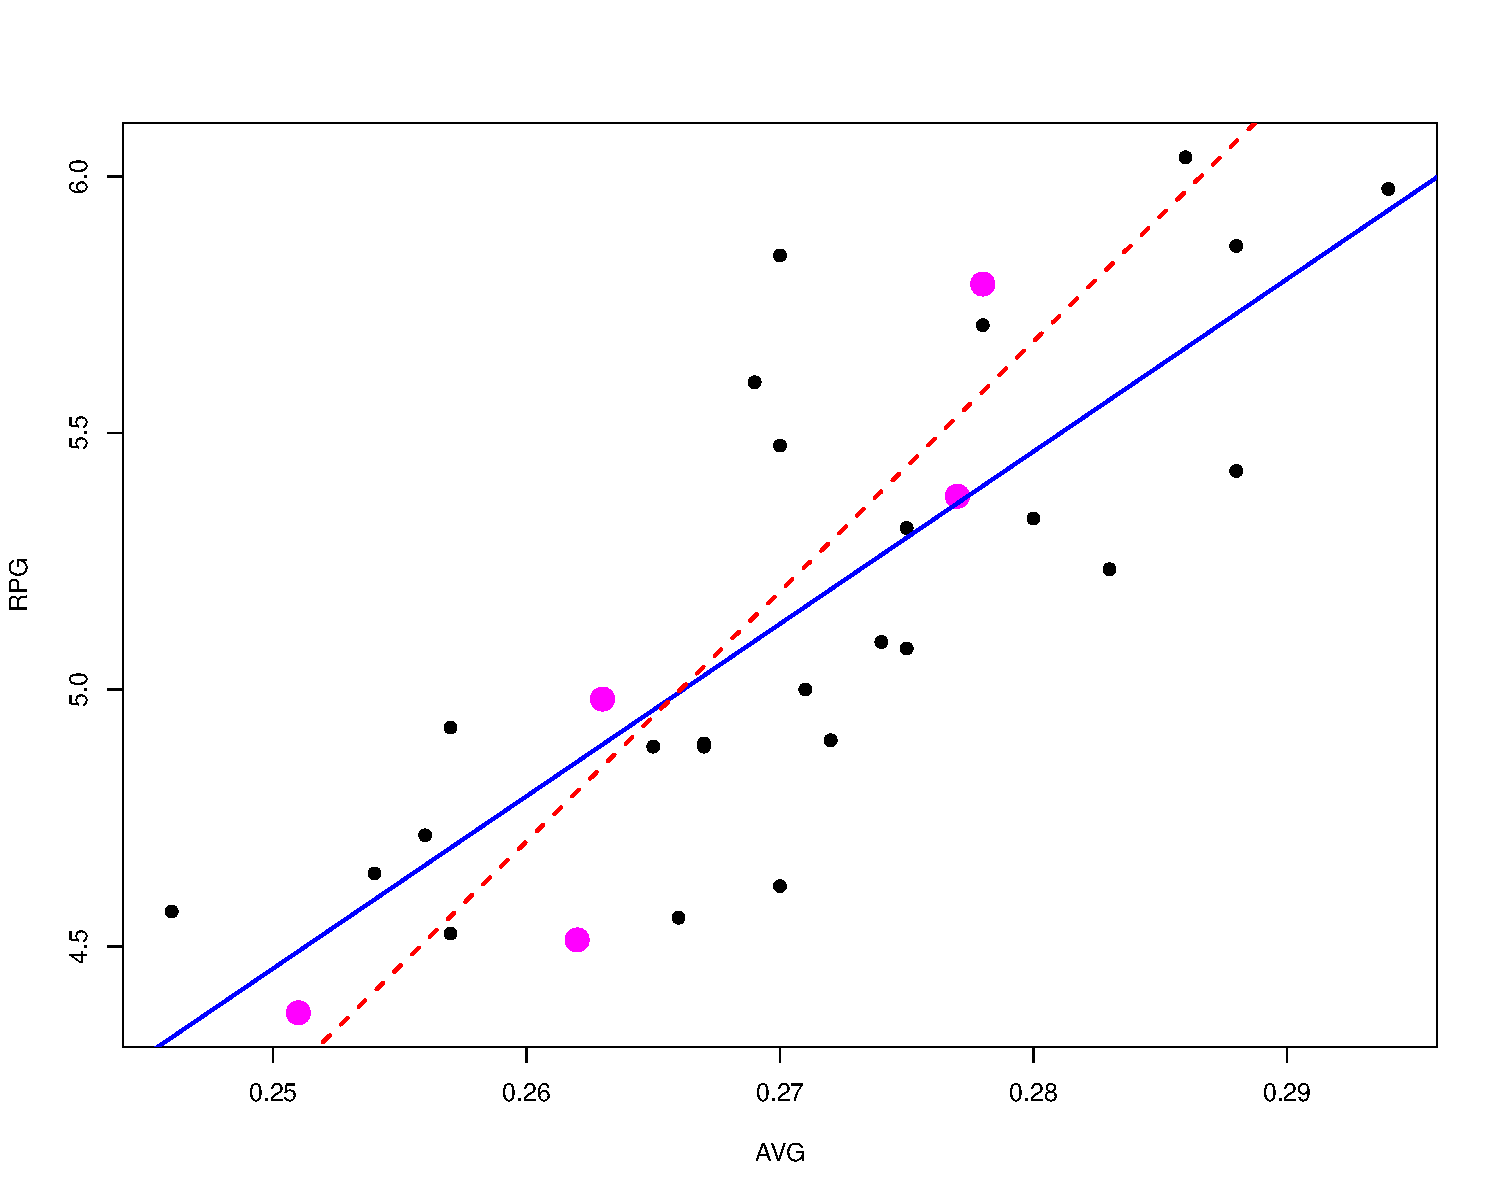
\includegraphics[scale=.3,angle=0]{figures/subsamp-avg.pdf}
%\end{center}
%
%\vspace{-5mm}
%In summary, we need to work with the notion of a {\color{blue}``true line''} and a {\color{blue}probability distribution} that describes deviation around the line.
%\end{frame}
%
%
%
%
%\begin{frame}
%\frametitle{The simple linear regression model} \vspace{-0.5cm}
%
%The power of statistical inference comes from the ability to make
%precise statements about the accuracy of the forecasts. 
%
%\sk
%In order to do this we must invest in a \rd probability model\bk .
%
%\sk {\large
%\bl Simple Linear Regression Model:
%$Y = \beta_0 + \beta_1 X + \varepsilon$ \rd
%\large
%\[
%\varepsilon \sim \mr{N}(0, \sigma^2) 
%\]}
%
%\vspace{-0.5cm}
%\begin{itemize}
%\item $\beta_0 +\beta_1 X$ represents the ``true line''; The part of $Y$ that depends on $X$.
%\item The error term $\varepsilon$ is independent ``idosyncratic noise''; The part of $Y$ not associated with $X$.
%
%\end{itemize}
%\end{frame}
%
%%%%%%%%%%%%%%%%%%%%%%%%%%%%%%%%%%%%%%%%%%%%%
%
%\begin{frame}
%\frametitle{Visually, what is going on here?} 
%
%%$$
%%Y = \beta_0 + \beta_1 X + \varepsilon
%%$$
%
%%\vspace{-1cm}
%
%
%\begin{center}
%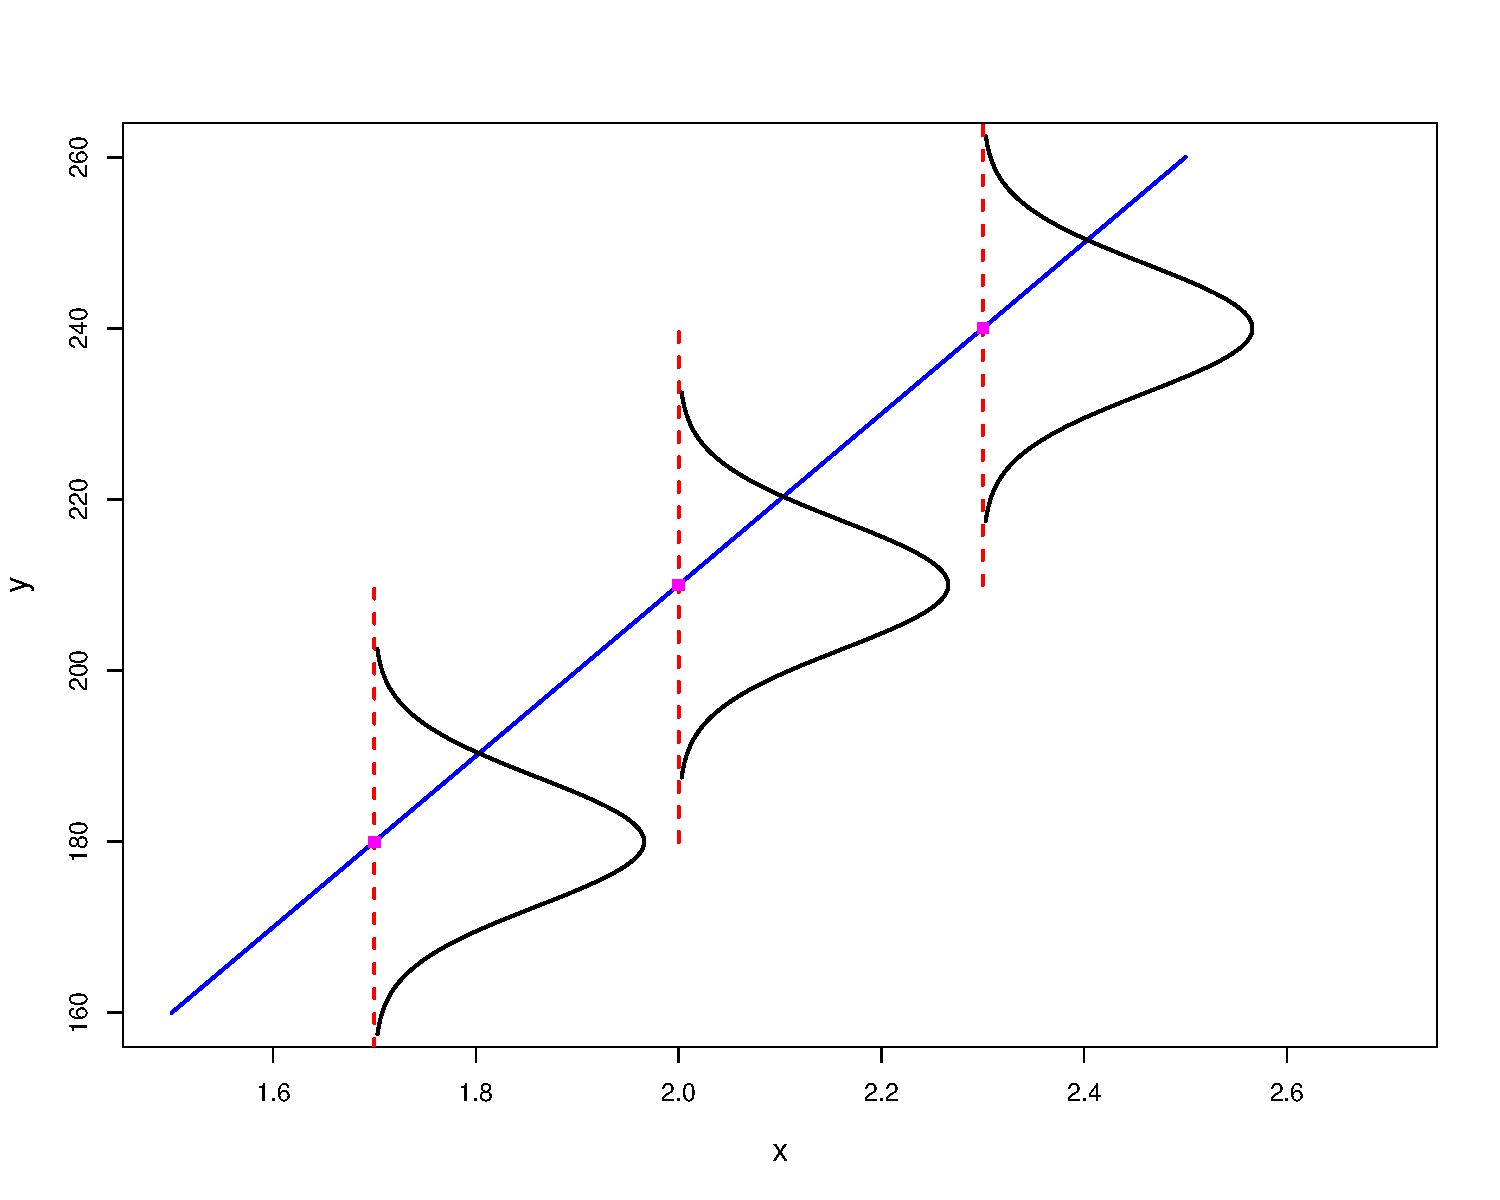
\includegraphics[width=3.7in]{figures/norm-cond-dist.pdf}
%\end{center}
%
%
%%\vspace{-0.5cm}
%%The conditional distribution for $Y$ given $X$ is Normal:
%%
%%\vspace{-0.5cm}
%%
%%\[ \rd Y | X\sim \mr{N}(
%%\beta_0 + \beta_1 X, \sigma^2)\bk.
%%\]
%
%\end{frame}
%%%%%%%%%%%%%%%%%%%%%%%%%%%%%%%%%%%%%%%%%%
%
%%%%%%%%%%%%%%%%%%%%%%%%%%%%%%%%%%%%%%%%%%%%%
%\begin{frame}
%\frametitle{The simple linear regression model -- example}
%
%You are told (without looking at the data) that
%\begin{center}
%$\beta_0 = 40$; $\beta_1= 45$; $\sigma = 10$ 
%\end{center}
%and you are asked to
%predict price of a 1500 square foot house.  
%
%\sk
%What do you know about $Y$ from the model?
%\begin{eqnarray*}
%Y &=& 40 + 45(1.5) + \varepsilon\\
%&=& 107.5 + \varepsilon
%\end{eqnarray*}
%Thus \bl our prediction for price is \rd
%$Y | (X=1.5)\sim \mr{N}(107.5, 10^2)$
%
%
%\bk
%and a $95\%$ {\it Prediction Interval} for Y is  \rd  $87.5 < Y < 127.5$
%
%\end{frame}
%
%%%%%%%%%%%%%%%%%%%%%%%%%%%%%%%%%%%%%%%%%%%%%
%\begin{frame}
%\frametitle{In picture form, our model tells us about uncertainty} 
%
%\vspace{-2mm}
%$$
%Y = \beta_0 + \beta_1 X + \varepsilon
%$$
%
%\vspace{-8mm}
%
%\begin{center}
%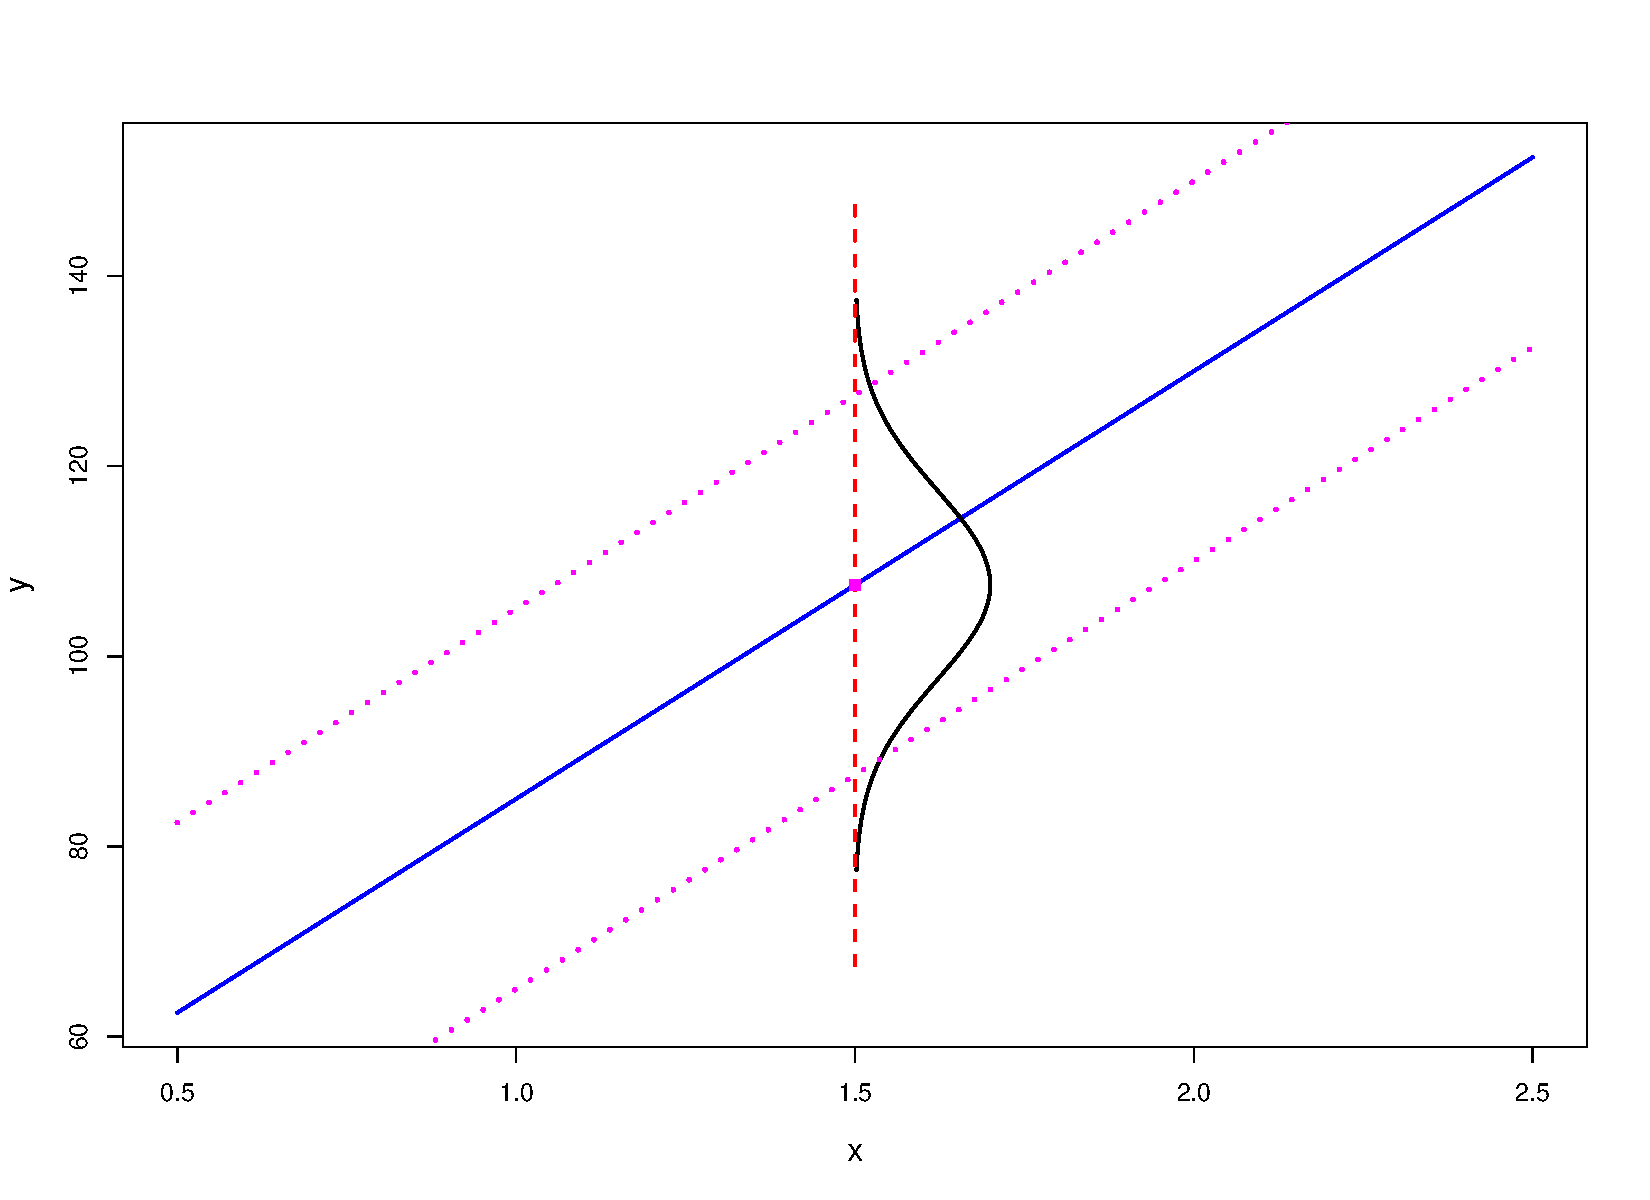
\includegraphics[width=3.7in]{figures/norm-cond-dist-2.pdf}
%\end{center}
%
%\vspace{2mm}
%
%\vspace{-0.5cm}
%The conditional distribution for $Y$ given $X$ is Normal:
%
%\vspace{-3mm}
%\[ \rd Y | X=x\sim \mr{N}(
%\beta_0 + \beta_1 x, \sigma^2)\bk.
%\]
%
%\end{frame}
%%%%%%%%%%%%%%%%%%%%%%%%%%%%%%%%%%%%%%%%%%
%
%
%%\begin{frame}
%%\frametitle{Conditional distributions}
%%
%%The model says that the mean value of a 1500 sq. ft. house is
%%\$107,500 and that deviation from mean is within $\approx$ \$20,000.
%%
%%\sk\sk
%%We are 95\% sure that
%%\bi
%%\p
%%$-20 < \varepsilon < 20$
%%\p $87.5 < Y < 127.5$
%%\ib
%%
%%\sk\sk In general, the 95 \% \rd P\bk rediction \rd I\bk nterval 
%%is \rd PI $ = \beta_0 +
%%\beta_1 X \pm 2\sigma$.
%%
%%\bk
%%
%%\end{frame}
%%%%%%%%%%%%%%%%%%%%%%%%%%%%%%%%%%%%%%%%%%%%
%
%
%
%
%
%
%%%%%%%%%%%%%%%%%%%%%%%%%%%%%%%%%%%%%%
%
%\begin{frame}
%\frametitle{Why do we choose this probability model?} \vspace{-0.5cm}
%
%
%Put differently, why do we have $\varepsilon \sim \mr{N}(0,\sigma^2)$?  \sk
%\bi 
%\p $E[\varepsilon] = 0 \Leftrightarrow E[Y \mid X] = \beta_0 +
%\beta_1 X$\\
% ($E[Y \mid X] $ is \bl ``conditional expectation of $Y$
%given $X$''\bk).  
%\p Many things are close to Normal (central limit
%theorem).  
%\p It works!  This is a very robust model for the world.  
%\ib
%
%\rd
%\sk We can think of $\beta_0 + \beta_1 X$ as the ``true'' regression line.
%
%\end{frame}
%%%%%%%%%%%%%%%%%%%%%%%%%%%%%%%%%%%%%%%
%
%%%%%%%%%%%%%%%%%%%%%%%%%%%%%%%%%%%%%%%%
%%%%%%%%%%%%%%%%%%%%%%%%%%%%%%%%%%%%%%%%%%%%%%%%
%%\begin{frame}
%%\frametitle{Conditional Distributions} \vspace{-0.5cm}
%%
%%Regression models are really all about modeling the 
%%conditional distribution of $Y$ given $X$.
%%
%%\sk \rd 
%%Why are conditional distributions important?  \bk
%%
%%
%%\sk
%%Given that I know $X$ what kind of $Y$ can I expect? Our model provides one way to think about this question. 
%%
%%\sk We can also look at this  by \rd``slicing'' \bk the
%%cloud of points in the scatterplot to obtain the distribution of $Y$ conditional
%%on various ranges of $X$ values.
%%\end{frame}
%%%%%%%%%%%%%%%%%%%%%%%%%%%%%%%%%%%%%%%%%%%%%%%%%%
%%
%%\begin{frame}
%%\frametitle{Data Conditional Distribution vs Marginal Distribution}
%%
%%
%%Let's consider a regression of house \bl price \bk on \bl size\bk:
%%
%%\sk
%% \includegraphics[width=4.5in]{cndprice}
%%
%%\end{frame}
%%%%%%%%%%%%%%%%%%%%%%%%%%%%%%%%%%%%%%%%%%%%%%%%%%%%
%%
%%\begin{frame}
%%\frametitle{Conditional Distribution and Marginal Distribution}\vspace{-0.5cm}
%%
%%Key Observations from these plots:
%%\bi
%%\p Conditional distributions answer the forecasting problem:
%% if I know that a house is between 1 and 1.5 1000 sq.ft., 
%%then the conditional distribution (second boxplot) 
%%gives me a point forecast (the mean) and prediction interval.
%%\p The conditional means seem to line up along the regression line.
%%\p The conditional distributions have much smaller dispersion 
%%than the marginal distribution.
%%\ib
%%
%%\end{frame}
%%%%%%%%%%%%%%%%%%%%%%%%%%%%%%%%%%%%%%%%%%%%%%%%%%%%%
%%
%%
%%\begin{frame}
%%\frametitle{Conditional Distribution vs Marginal Distribution}\vspace{-0.5cm}
%%
%%This suggests two general points:
%%\bi
%%\p If X has no forecasting power, then
%%the marginal and conditionals will be the same.
%%\p
%%If X has some forecasting information, then
%%conditional means will be different than the marginal or overall mean
%%and conditional standard deviation of Y given X will be less than the
%%marginal standard deviation of Y.
%%\ib
%%\end{frame}
%%%%%%%%%%%%%%%%%%%%%%%%%%%%%%%%%%%%%%%%%%%%%%%%%%%%%%
%%
%%
%%\begin{frame}
%%\frametitle{Conditional Distribution vs Marginal Distribution}\vspace{-0.5cm}
%%
%%Intuition from an example where X has no predictive power.
%%
%%\sk
%% \includegraphics[width=4.5in]{stopsign}
%%
%%\end{frame}
%%
%%
%%%%%%%%%%%%%%%%%%%%%%%%%%%%%%%%%%%%%%%%%%%%%%
%
%\begin{frame}
%\frametitle{The importance of $\sigma$}
%
%\sk
%The conditional distribution for $Y$ given $X$ is Normal:
%\[ \rd Y | X\sim \mr{N}(
%\beta_0 + \beta_1 X, \sigma^2)\bk.
%\]
%\vskip -.8cm
%$\sigma$ controls \bl dispersion\bk:
%\begin{center}
%\hspace*{-5mm}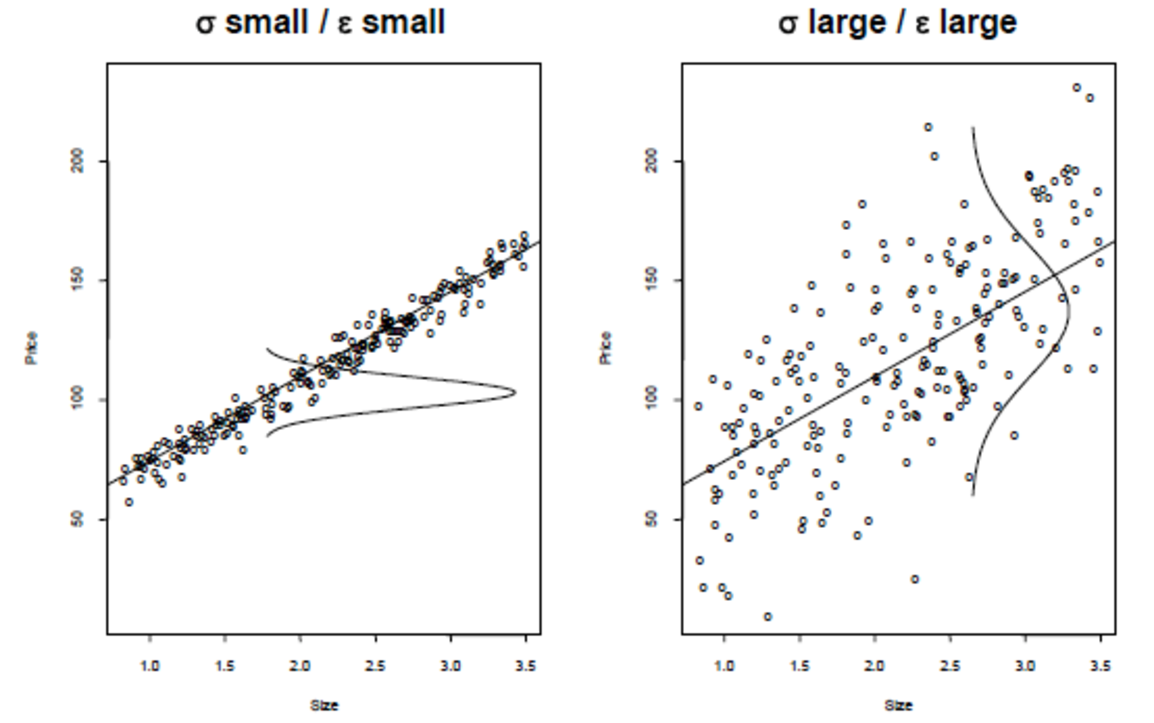
\includegraphics[width=3.7in]{figures/cnd.pdf}
%\end{center}
%\end{frame}
%%%%%%%%%%%%%%%%%%%%%%%%%%%%%%%%%%%%%%%%%%
%
%
%\begin{frame}
%\frametitle{Digging into the moments of the SLR model} \vskip -.5cm
%
%More on the conditional distribution:
%\[\rd Y | X\sim \mr{N}(
%E[Y | X], \mr{var}(Y|X) )\bk. \]
%\vskip -1cm
%\bi
%\p The conditional mean is 
%$E[Y|X] = E[\beta_0 + \beta_1 X + \varepsilon] =  \beta_0 +
%\beta_1 X$.
%\p The conditional variance is $ 
%\mr{var}(Y|X) = \mr{var}(\beta_0 + \beta_1 X + \varepsilon) = \mr{var}(\varepsilon) 
%= \sigma^2$.
%\ib
%
%
%\bi
%\p $\sigma^2< \mr{var}(Y ) $ if $X$ and $Y$ are related.
%\ib
%
%\end{frame}
%
%\begin{frame}
%\frametitle{Summary of simple linear regression}
%
%Assume that  all observations are drawn from our regression model
%and that errors on those observations are independent.
%
%\sk The model is
%\[ Y_i =\beta_0 + \beta_1 X_i + \varepsilon_i
%\]
%where $\varepsilon$ is independent and identically distributed
%$\mr{N}(0,\sigma^2)$.
%
%
%\bi
%\p {\color{burntorange}independence} means that knowing $\varepsilon_i$ doesn't affect your views about $\varepsilon_j$
%\p {\color{burntorange} identically distributed} means that we are using the same Normal for every $\varepsilon_i$
%\ib
%\end{frame}
%%%%%%%%%%%%%%%%%%%%%%%%%%%%%%%%%%%%%%%%%%%
%
%%%%%%%%%%%%%%%%%%%%%%%%%%%%%%%%%%%%%%%%%%%%
%
%%\begin{frame}
%%\frametitle{Summary of simple linear regression}
%%
%%\sk The model is
%%\[ Y_i =\beta_0 + \beta_1 X_i + \varepsilon_i
%%\]
%%$\varepsilon_i \sim \mr{N}(0,\sigma^2)$.
%%
%%\sk The SLR has 3 basic parameters: 
%%\bi
%%\p$\beta_0$, $\beta_1$ (linear
%%pattern)
%%\p $\sigma$ (variation around the line).
%%\ib
%%\end{frame}
%%%%%%%%%%%%%%%%%%%%%%%%%%%%%%%%%%%%%%%%%%%
%
%
%
%\begin{frame}
%\frametitle{Key characteristics of linear regression model}
%
%
%\bi
%\p Mean of $Y$ is \bl linear \bk in $X$. \sk
%\p Error terms (deviations from line) are \bl Normally distributed \bk 
%(very few deviations are more than $2$ standard devations away from the regression mean). \sk
%\p Error terms have \bl constant variance\bk.
%\ib
%
%\end{frame}
%
%%%%%%%%%%%%%%%%%%%%%%%%%%%%%%%%%%%%%%%%%%
%
%\begin{frame}
%\frametitle{Estimation for the SLR model} 
%
%
%SLR assumes every observation in the dataset was generated
%by the model:
%\[
%Y_i = \beta_0 + \beta_1 X_i + \varepsilon_i
%\]
%
%\sk
%This is a model for the conditional distribution of Y
%given X.
%
%\sk
%We use Least Squares {\color{burntorange}{\it to estimate}} $\beta_0$ and $\beta_1$:
%\[ \hat{\beta}_1 = b_1 = r_{xy} \times \frac{s_y}{s_x}  
%\]
%\[
%\hat{\beta}_0 = b_0 =  \bar{Y} - b_1 \bar{X}
%\]
%\end{frame}
%%%%%%%%%%%%%%%%%%%%%%%%%%%%%%%%%%%%%%%%%%%
%
%
%%\begin{frame}
%%\frametitle{Estimation for the SLR Model} 
%%
%%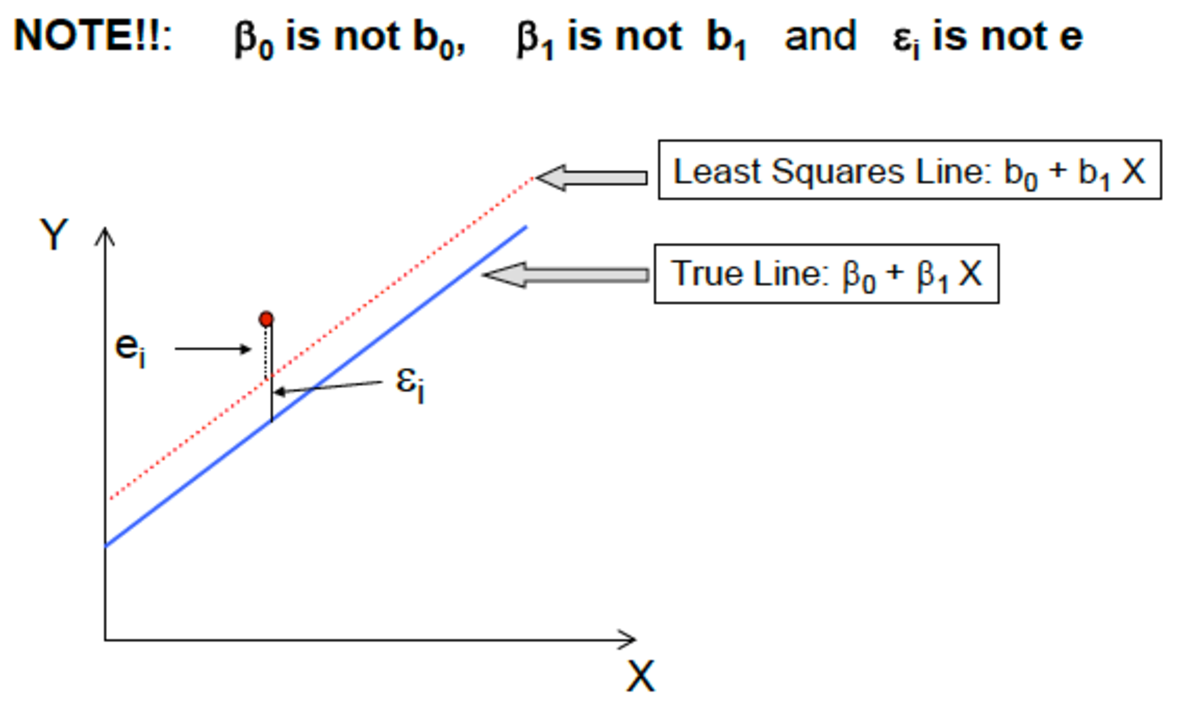
\includegraphics[width=4.5in]{figures/slide3}
%%\end{frame}
%
%
%%%%%%%%%%%%%%%%%%%%%%%%%%%%%%%%%%%%%%%%%%%
%%\begin{frame}
%%\frametitle{Estimation of Error Variance} 
%%
%%Recall that $\varepsilon_i \stackrel{iid}{\sim} N(0, \sigma^2)$,
%%and that $\sigma$ drives the width of the prediction intervals:\rd
%%\[
%%\sigma^2 = \var(\varepsilon_i) 
%%= E[(\varepsilon_i - E[\varepsilon_i])^2] =
%%E[\varepsilon_i^2]
%%\] \bk
%%
%%A sensible strategy would be to estimate the average
%%for squared errors with the sample average squared residuals:\bl
%%\[
%%\hat{\sigma}^2 = \frac{1}{n} \sum_{i=1}^n e_i^2
%%\]
%%
%%\end{frame}
%%%%%%%%%%%%%%%%%%%%%%%%%%%%%%%%%%%%%%%
%
%
%\begin{frame}
%\frametitle{Estimation of error variance} 
%\vspace{-0.5cm}
%
%We estimate $s^2$ with: {\color{blue}
%\[
%s^2 = \frac{1}{n-2} \sum_{i=1}^n e_i^2 = \frac{SSE}{n-2}
%\]}
%(\rd$2$ \bk is the number of regression coefficients; i.e. \rd 2 \bk for  $\beta_0$ and
%$\beta_1$).
%
%\sk
%We have $n-2$ degrees of freedom because 2 have been ``used up'' in
%the estimation of $b_0$ and $b_1$.
%
%\sk
%We usually  use \rd$s = \sqrt{SSE/(n-2)}$\bk, in the same units as $Y$. It's also called the {\color{burntorange} \bf regression standard error}.
%
%\end{frame}
%
%\begin{frame}
%	\frametitle{Uncertainty in estimates}
%	We now know how to make statements about \bo{uncertainty} in forecasts \dg{aka} predictions.  But what about our \lb{parameter estimates}?
%	
%	\sk\sk
%	
%	{\bf Q:} How much do our estimates depend on the 
%particular random sample that we happen to observe?
%\end{frame}
%
%\begin{frame}
%	\frametitle{Uncertainty in estimates}
%
%Imagine:\sk
%\bi
%\p Randomly draw different samples
%of the same size. 
%\p For each sample, compute
%the estimates $b_0$, $b_1$, and $s$.
%\ib
%
%\sk\sk\bl
%If the estimates don't vary much 
%from sample to sample, then
%it doesn't matter which sample you happen
%to observe. \rd\\ \sk
%If the estimates do vary a lot,
%then it matters which sample you happen
%to observe.
%
%\end{frame}
%
%
%\begin{frame}
%\frametitle{Sampling distribution of least squares estimates} 
%
%
%\hspace*{-7mm}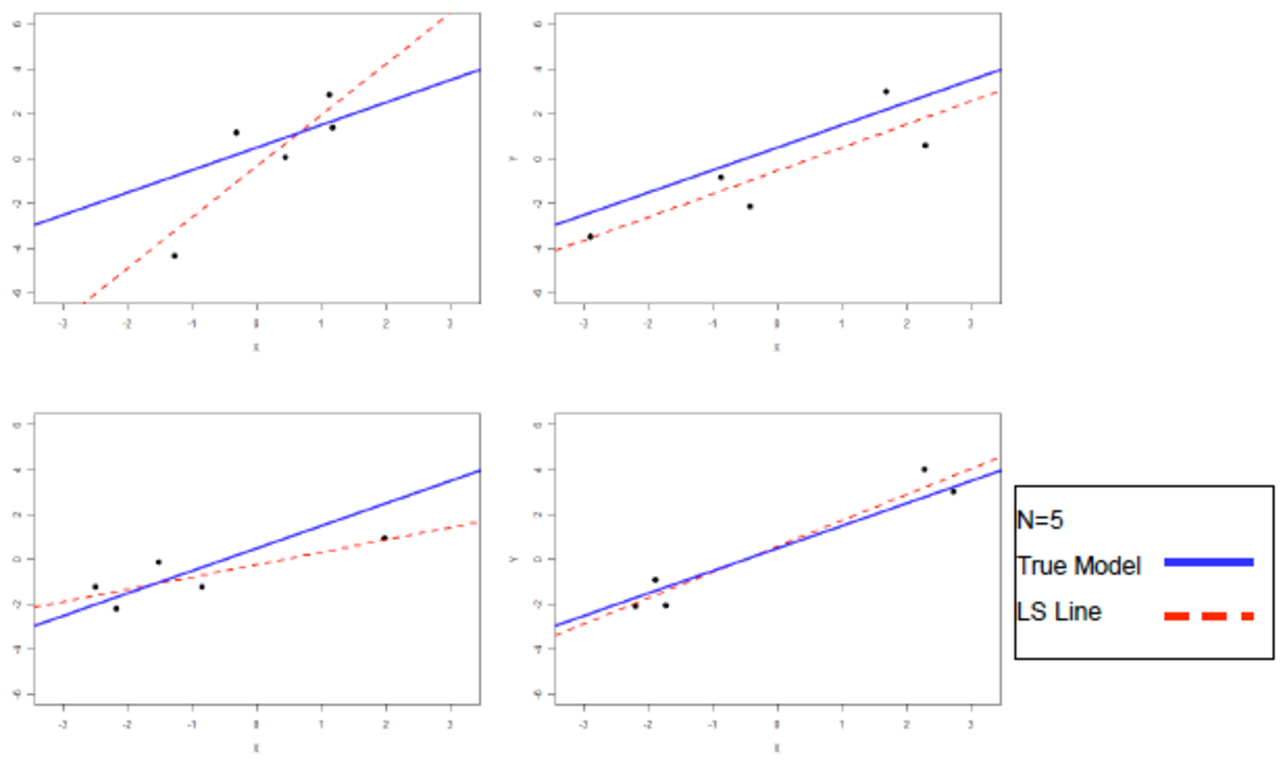
\includegraphics[width=4.8in]{figures/sampling1}
%
%\end{frame}
%%%%%%%%%%%%%%%%%%%%%%%%%%%%%%%%%%%%%%%
%
%\begin{frame}
%\frametitle{Sampling distribution of least squares estimates} 
%
%
%\hspace*{-7mm}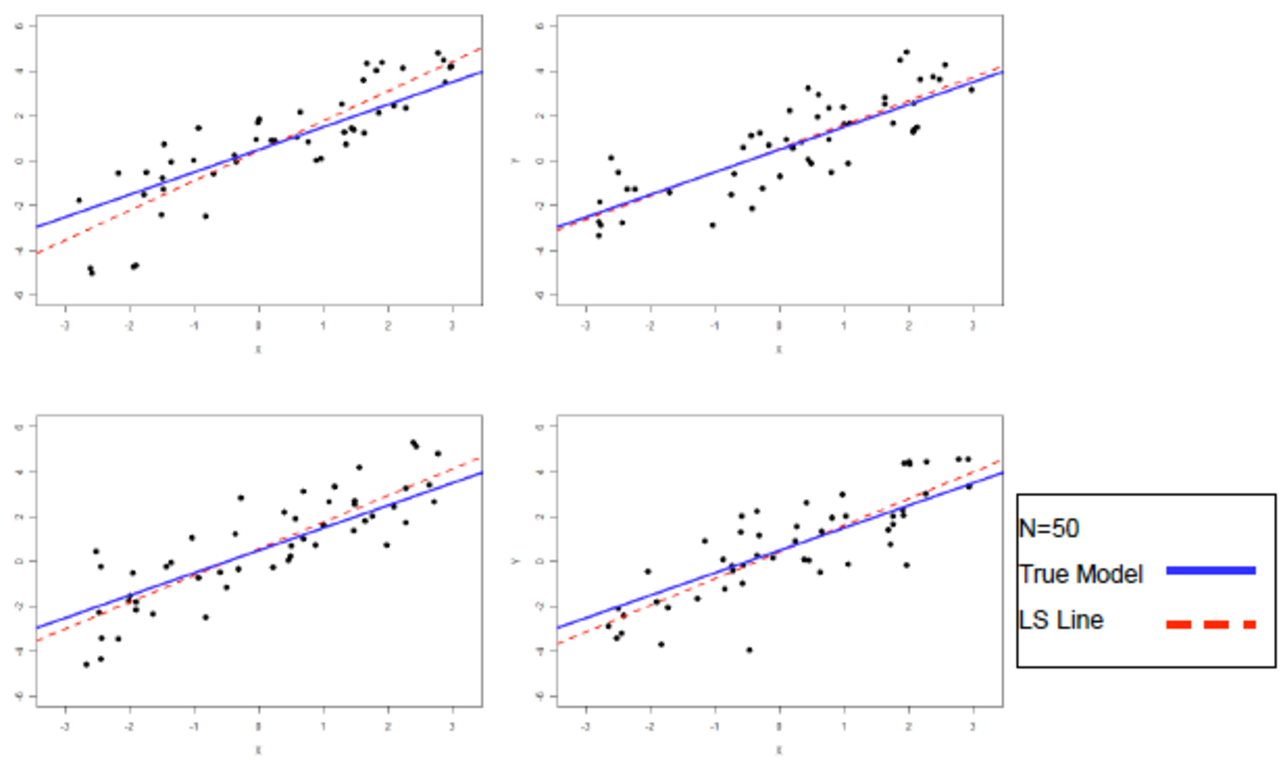
\includegraphics[width=4.8in]{figures/sampling2}
%
%\end{frame}
%%%%%%%%%%%%%%%%%%%%%%%%%%%%%%%%%%%%%%%
%
%
%\begin{frame}
%\frametitle{Sampling distribution of least squares estimates} 
%
%
%Least squares lines are much closer to the 
%true line when $N=50$.
%
%\sk
%For $N=5$,
%some lines are close, others aren't:
%\sk
%\begin{center}
% \rd {\bf We need to get ``lucky!''}\bk
%\end{center}
%
%\end{frame}
%
%\begin{frame}
%	\frametitle{So, to sum up ...}
%	Parameter estimates are \bo{\bf uncertain} because we only have sample from the population \\ \sk
%	We can characterize a \lb{\bf sampling distribution} of each parameter based on the assumptions of the SLR model \\ \sk
%	
%	  The standard deviation of the sampling distribution is called the \lb{\bf standard error} \\ \sk
%	  
%	  $\rightarrow$ {\tt R} directly reports standard errors.  They can also be calculated with other methods, like \dg{bootstrapping}.
%\end{frame}
%
%
%
%\begin{frame}
%\frametitle{Least squares -- {\tt R} output} 
%
%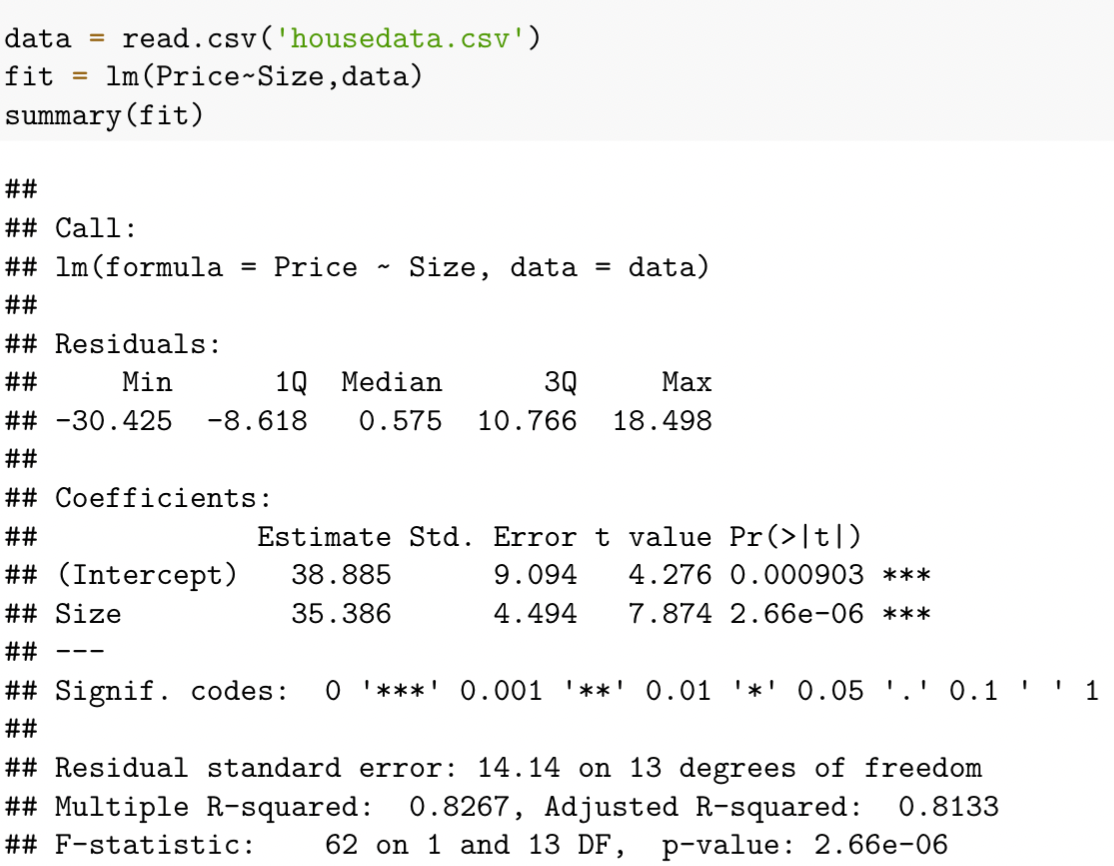
\includegraphics[scale=0.50]{figures/pred1}
%
%\end{frame}
%
%
%\begin{frame}
%\sk\sk
%	\dg{\bf The bootstrap }
%\end{frame}
%
%
%\begin{frame}
%	\frametitle{Quantifying uncertainty}
%In data science, we equate \lb{trustworthiness} with \lb{stability}: \\ \sk\sk
%
%\textbf{\bo{Key question:}}
%If our data had been different merely due to chance, would our answer have been different, too?
%Or would the answer have been stable, even with different data? \\ \sk\sk
%
%Confidence in your estimates $\iff$ Stability of those estimates under the influence of chance
%\end{frame}
%
%
%\begin{frame}
%	\frametitle{Example: Quantifying uncertainty}
%
%For example: \\ \sk\sk
%
%$\bo{\bullet}$ If doctors had taken a different sample of 503 cancer patients and gotten a drastically different estimate of the new treatment's effect, then the original estimate isn't very trustworthy. \\ \sk
%$\bo{\bullet}$ If, on the other hand, pretty much any sample of 503 patients would have led to the same estimates, then their answer for this particular subset of 503 is probably accurate.
%
%\end{frame}
%
%\begin{frame}
%	\frametitle{Some notation}
%	
%	Suppose we are trying to estimate some population-level feature of interest, $\theta$. This might be something very complicated! \sk \sk
%
%So we take a sample from the population: $X_1, X_2, \ldots, X_N$. We use the data to form an estimate $\hat{\theta}_N$ of the parameter. \\ \sk \sk {\bf \lb{ Key insight: $\hat{\theta}_N$ is a random variable.}} \\ \sk
%
%\dg{($\hat{\theta}_N$ can be the slope of a least squares regression)} \pause \\ \sk
%
%$\bo{\rightarrow}$ Now imagine repeating this process thousands of times! Since $\hat{\theta}_N$ is a random variable, it has a probability distribution: \bo{the sampling distribution}.
%	
%\end{frame}
%
%\begin{frame}
%	\frametitle{Visualizing this procedure}
%	\begin{center}
%	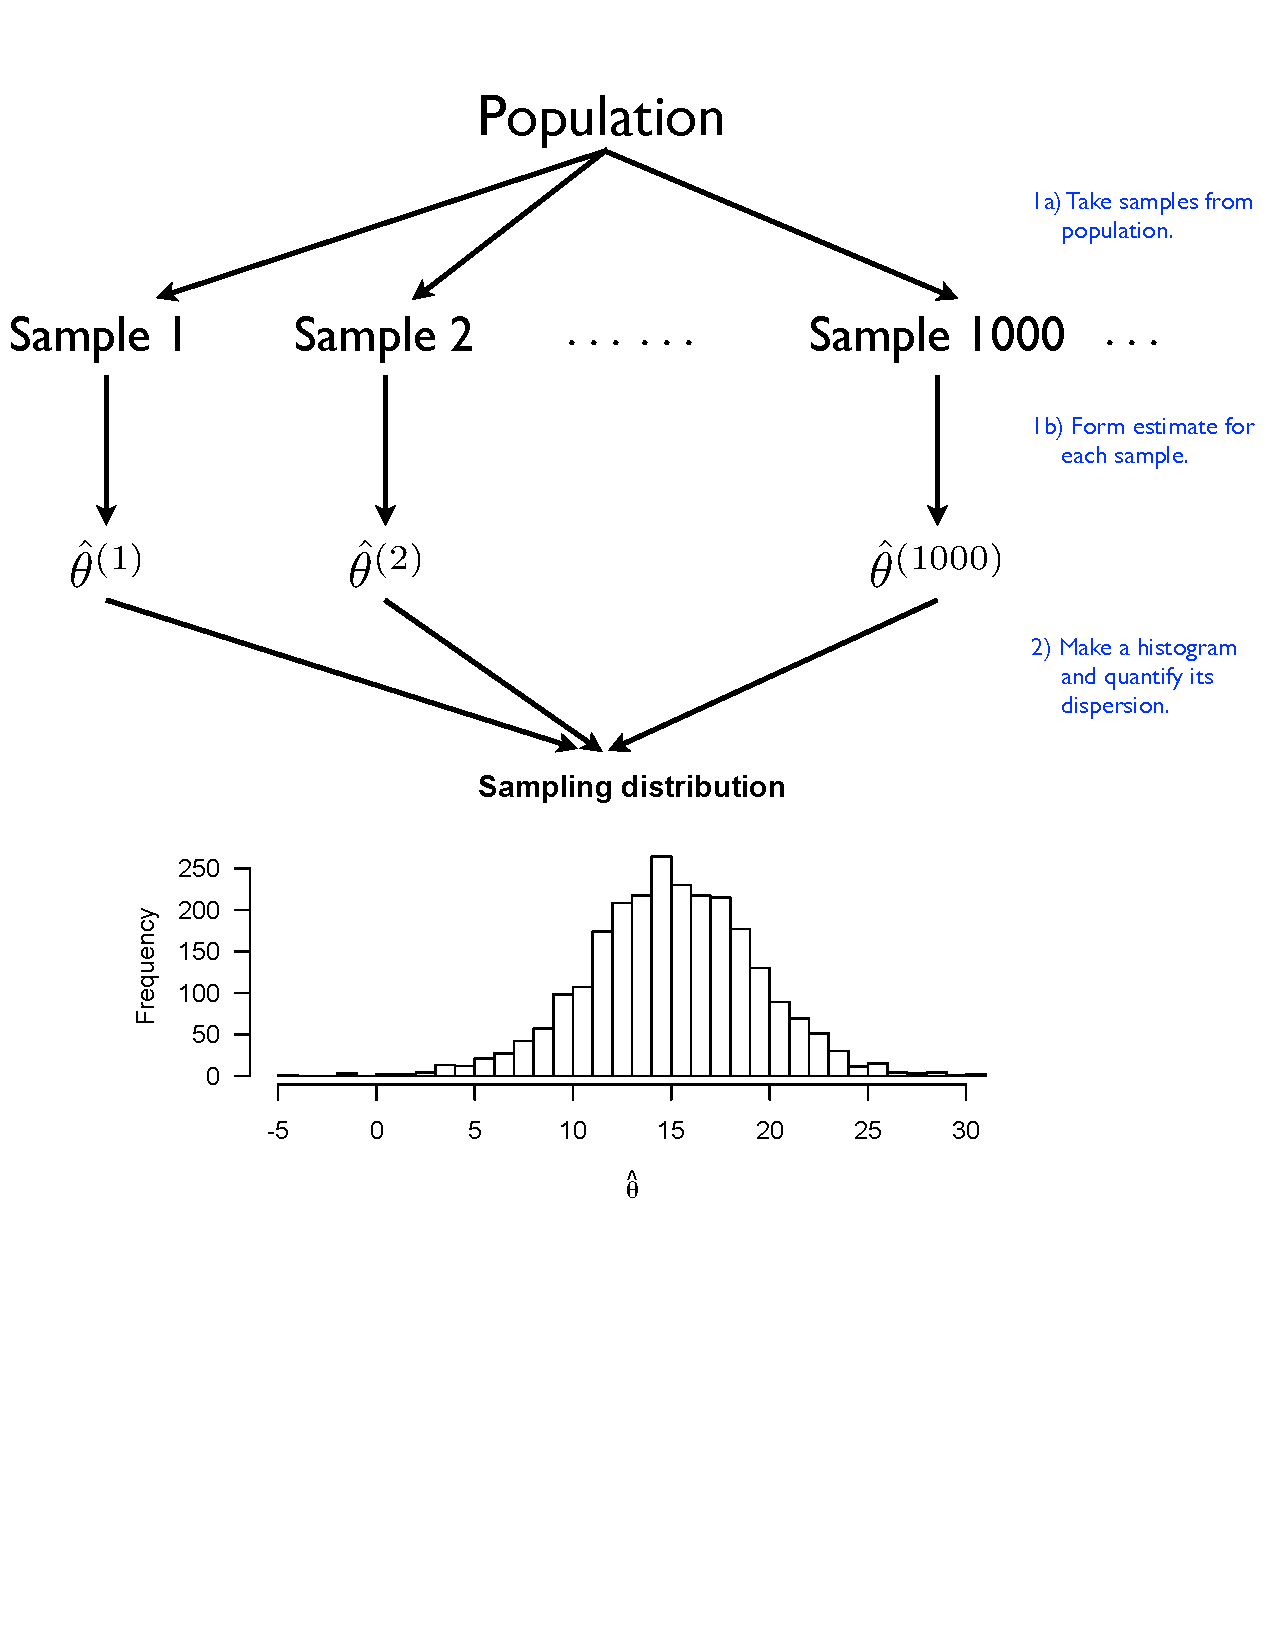
\includegraphics[scale=0.42]{figures/samplingdistribution_schematic}		
%	\end{center}
%\end{frame}
%
%\begin{frame}
%	\frametitle{Revisiting the standard error}
%	
%	\bo{Standard error}: the standard deviation of an estimator's sampling distribution:
%
%$$ \begin{aligned} \mbox{se}(\hat{\theta}_N) &= \sqrt{ \mbox{var}(\hat{\theta}_N) } \\ &= \sqrt{ E[ (\hat{\theta}_N - \bar{\theta}_N )^2] } \\ &= \mbox{Typical deviation of $\hat{\theta}_N$ from its average} \end{aligned} $$ \sk
%
%\lb{``If I were to take repeated samples from the population and use this estimator for every sample, how much does the answer vary, on average?''}
%\end{frame}
%
%
%\begin{frame}
%	\frametitle{Standard error}
%	
%	But there's a problem here... \\ \sk\sk
%
%Knowing the standard error requires knowing what happens across many separate samples.
%But we've only got our one sample! \\ \sk\sk
%{\bf So how can we ever calculate the standard error?}
%
%\end{frame}
%
%\begin{frame}
%\frametitle{Standard error}
%
%\begin{quote}
%	Two roads diverged in a yellow wood
%And sorry I could not travel both
%And be one traveler, long I stood
%And looked down one as far as I could
%To where it bent in the undergrowth...
%\end{quote}
%
%-- Robert Frost, The Road Not Taken, 1916 \\ \sk
%{\bf \lb{Quantifying our uncertainty would seem to require knowing all the roads not taken---an impossible task.}}
%\end{frame}
%
%\begin{frame}
%	\frametitle{The bootstrap}
%	
%{\bf Problem}: we can't take repeated samples of size $N$ from the population, to see how our estimate changes across samples. \\ \sk\sk
%
%{\bf \bo{Seemingly hacky solution}}: Take repeated samples of size $N$, with replacement, from the sample itself, and see how our estimate changes across samples. This is something we can easily simulate on a computer (with {\tt R}).\\ \sk\sk
%
%Basically, we pretend that our sample is the whole population and we charge ahead! This is called bootstrap resampling, or just bootstrapping.
%\end{frame}
%
%\begin{frame}
%	\frametitle{Sampling with replacement is key!}
%	
%	boostrapped sample 1 \sk
%	\begin{center}
%		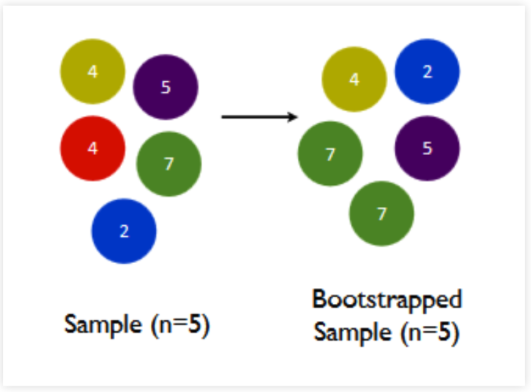
\includegraphics[scale=0.4]{figures/bs1}
%	\end{center}
%
%\end{frame}
%
%\begin{frame}
%	\frametitle{Sampling with replacement is key!}
%	
%	boostrapped sample 2 \sk
%	\begin{center}
%		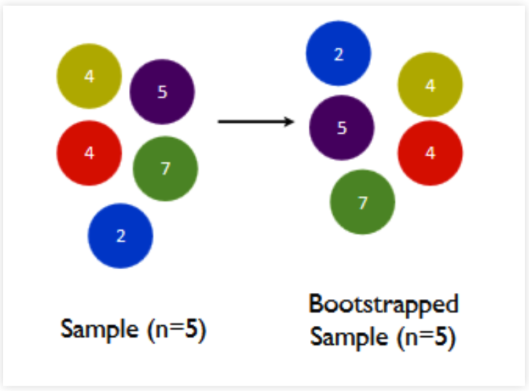
\includegraphics[scale=0.4]{figures/bs2}
%	\end{center}
%
%\end{frame}
%
%\begin{frame}
%	\frametitle{Sampling with replacement is key!}
%	
%	boostrapped sample 3 \sk
%	\begin{center}
%		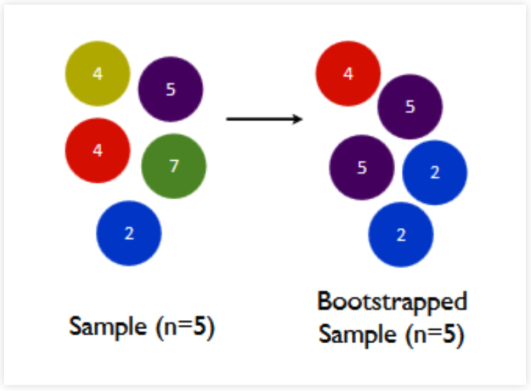
\includegraphics[scale=0.4]{figures/bs3}
%	\end{center}
%
%\end{frame}
%
%
%\begin{frame}
%	\frametitle{The true sampling distribution}
%	\begin{center}
%	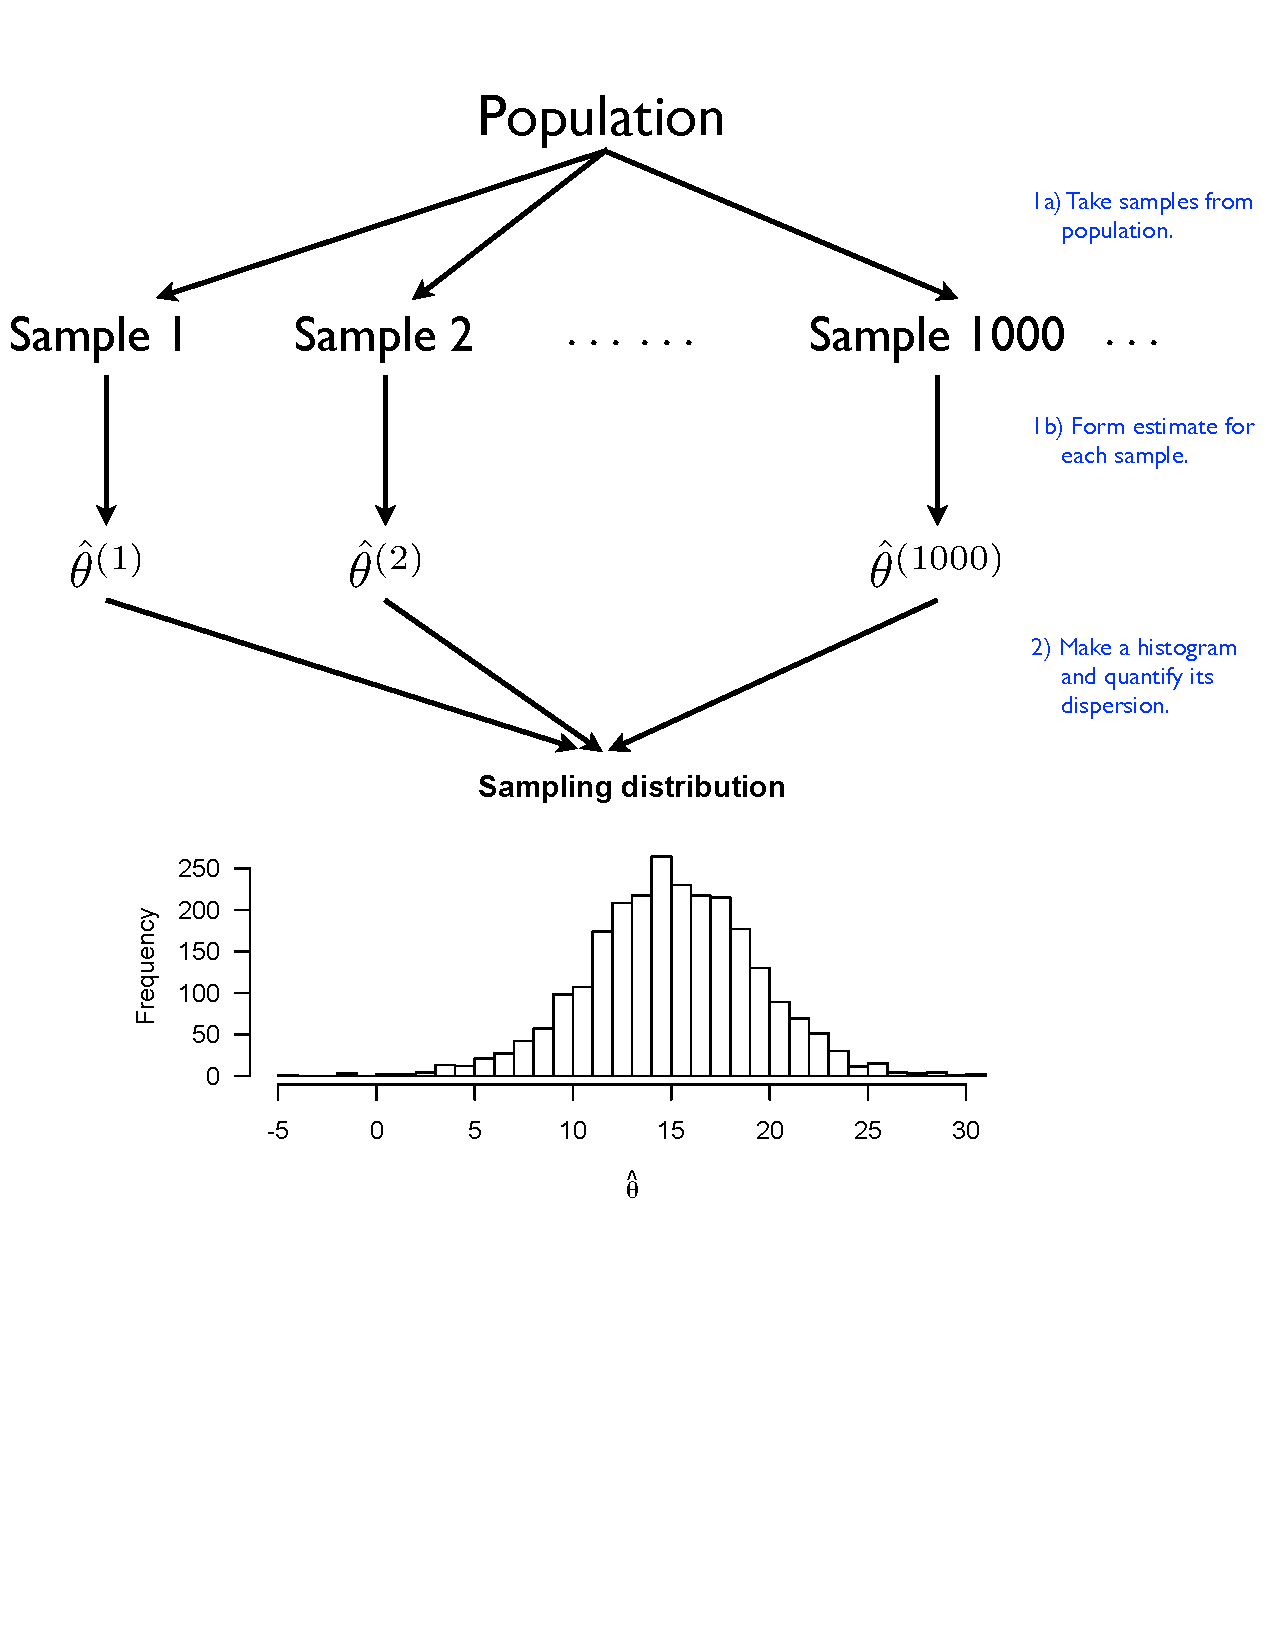
\includegraphics[scale=0.42]{figures/samplingdistribution_schematic}		
%	\end{center}
%\end{frame}
%
%\begin{frame}
%	\frametitle{The bootstrapped sampling distribution}
%	\begin{center}
%	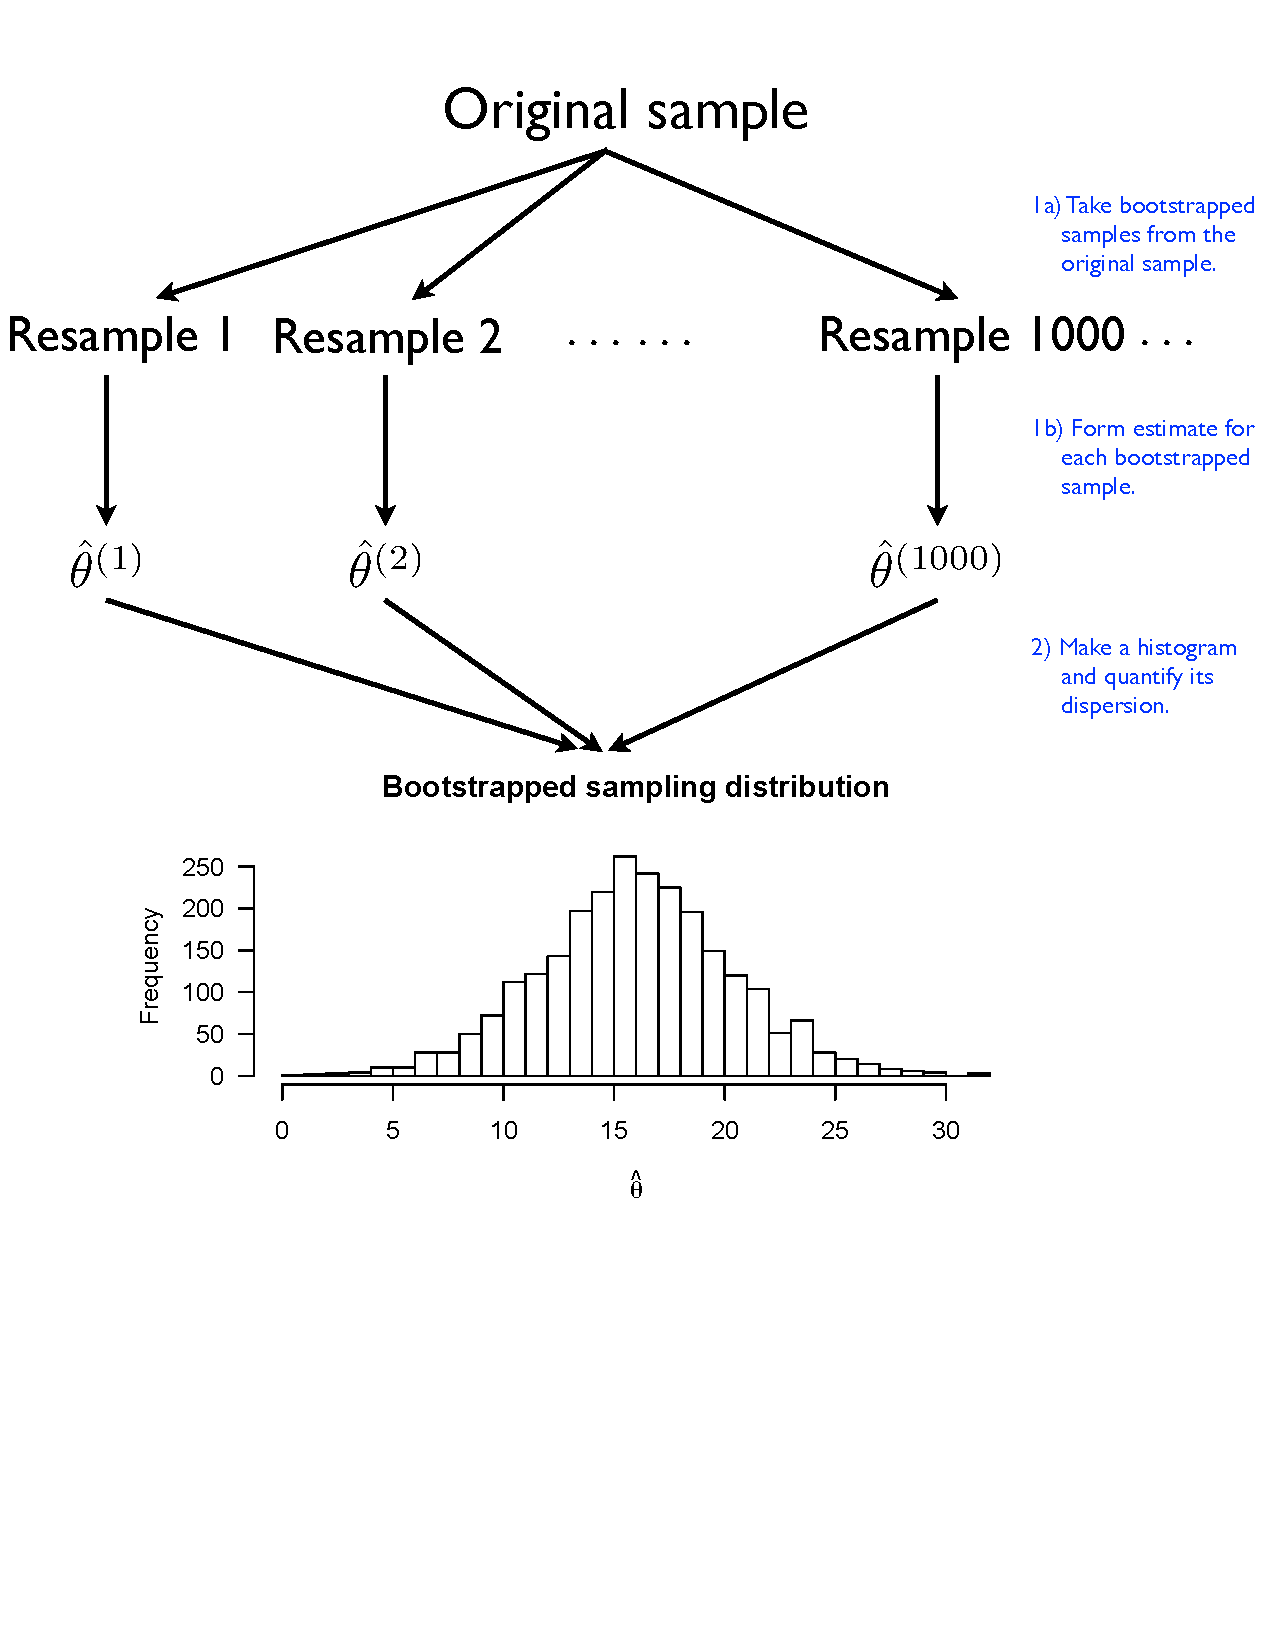
\includegraphics[scale=0.42]{figures/bootstrapping_schematic}		
%	\end{center}
%\end{frame}
%
%\begin{frame}
%	\frametitle{The bootstrapped sampling distribution}
%\bo{$\bullet$} Each bootstrapped sample has its own pattern of duplicates and omissions from the original sample. \\ \sk\sk
%
%\bo{$\bullet$} These duplicates and omissions create variability in $\hat{\theta}$ from one bootstrapped sample to the next. \\ \sk\sk
%
%\bo{$\bullet$} This variability mimics the true sampling variability you'd expect to see across real repeated samples from the population. \\ \sk\sk
%
%Let's check out {\tt bootstrap.R} to see this in action!
%
%\end{frame}

\begin{frame}
\sk\sk
	\dg{\bf Multiple linear regression }
\end{frame}


\begin{frame}
\frametitle{Multiple linear regression}

Many problems involve more than one independent variable 
or factor which affects the dependent or response variable.

\sk
\bi 
\p More than size to predict house price!
\p Demand for a product given prices of competing brands, 
advertising, household attributes, etc.
\ib 

\sk
In SLR, the conditional mean of $Y$ depends on $X$. The 
Multiple Linear Regression (MLR) model extends this idea to include more 
than one independent variable.
\end{frame}

\begin{frame}
\frametitle{The MLR model}

\sk
Same as always, but with more covariates.

{\bl  \large
\[ Y = \beta_0 + \beta_1 X_1 + \beta_2 X_2 + \dots + \beta_p X_p + \epsilon 
\]}

Recall the key structural assumption of our linear regression model: \\ \sk


$\rightarrow$ The conditional mean of $Y$ is \rd linear \bk in the $X_j$ variables. \\ \sk
%$\rightarrow$  The errors (deviations from line) \\ 
%\begin{itemize}
%	\item are normally distributed \vspace{-2mm}
%	\item independent from each other \vspace{-2mm}
%	\item identically distributed (i.e., they have constant variance) \vspace{-2mm}
%\end{itemize} 
%
%
%{\bl  \large 
%\[ Y |(X_1\ldots X_p) \sim N(\beta_0 + \beta_1 X_1 \ldots + \beta_p X_p, \sigma^2)
%\]}

\end{frame}
%%%%%%%%%%%%%%%%%%%%%%%%%%%%%%%%%%%%%%%%%



\begin{frame}
\frametitle{The MLR model}  

Our interpretation of regression coefficients can be extended from the
simple  single covariate regression case: \sk

{\bl  \large 
\[ \beta_j = \frac{\partial E[Y | X_1,\ldots,X_p]}{\partial X_j} \] }
\sk
\begin{center}\rd \vspace{-.3cm}
Holding all other variables constant\bk, $\beta_j$ is the \\
average  change in $Y$ per unit change in $X_j$.
\end{center}

\end{frame}


%%%%%%%%%%%%%%%%%%%%%%%%%%%%%%%%%%%%%%%%

\begin{frame}
\frametitle{The MLR model}

\sk
If $p=2$, we can plot the regression surface in 3D. \\ \sk

Consider  sales of a product as predicted by price of this 
product ({\bl P1}) and the price of a competing product ({\rd P2}). 


$$
Sales = \beta_0 + \beta_1 P1 + \beta_2 P2 + \epsilon
$$
\vspace{-0.7cm}
\begin{center}
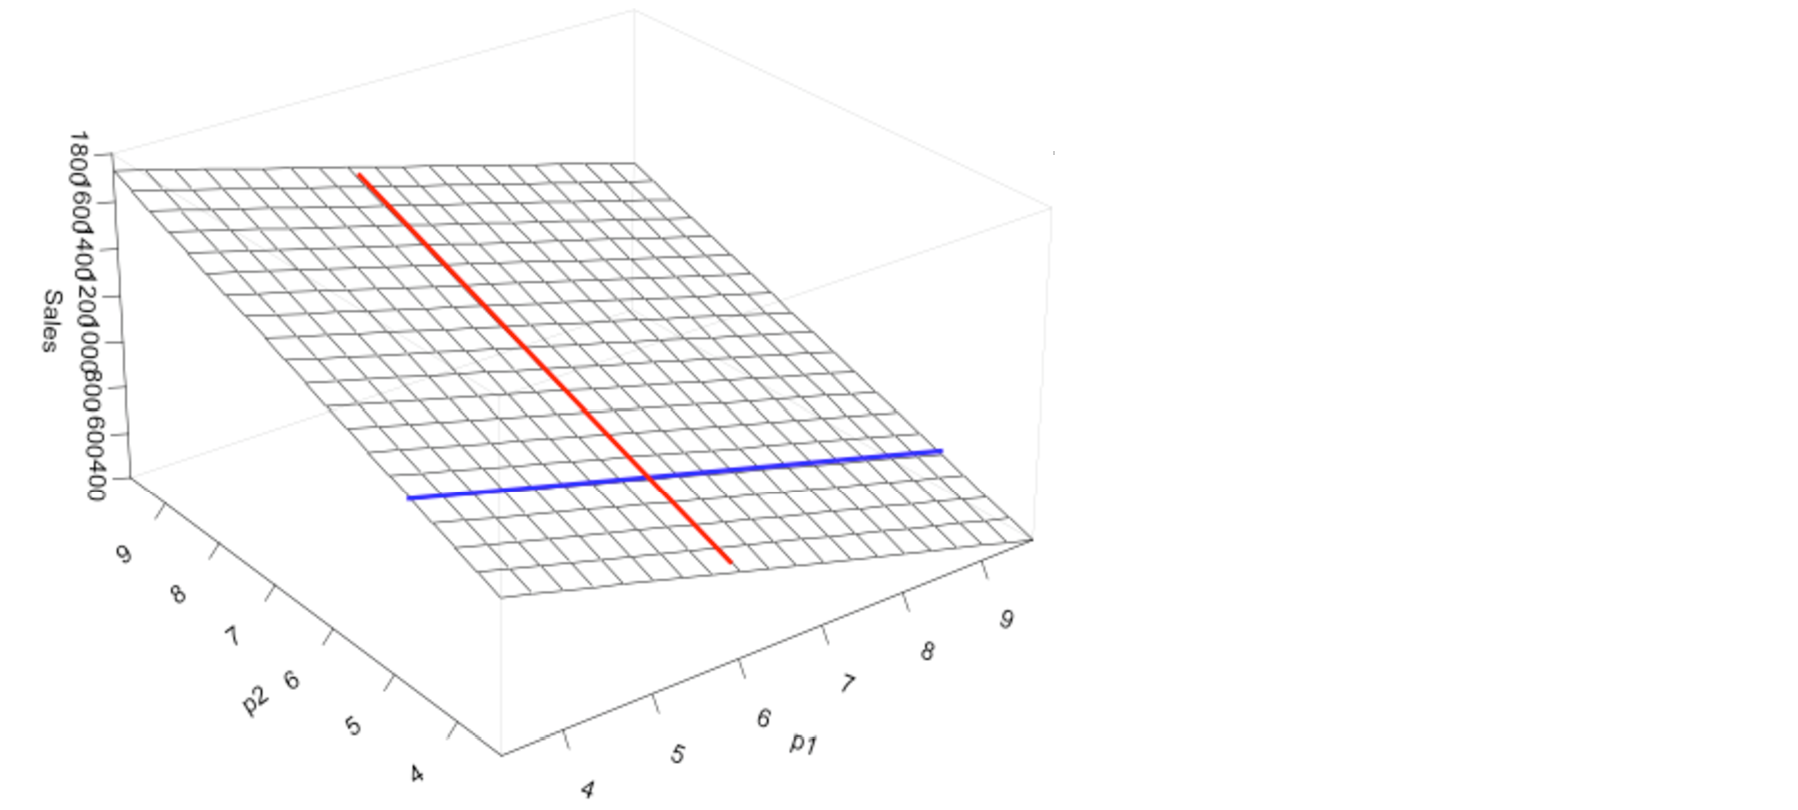
\includegraphics[width=2.5in]{figures/plane}
\end{center}
\end{frame}

\begin{frame}
\frametitle{Least squares again!}  

\[\bl \large Y  = \beta_0 + \beta_1 X_1 \ldots
+ \beta_p X_p + \varepsilon\]

\sk
{\bf How do we estimate the MLR model parameters?}

\sk
The principle of \bo{least squares} is exactly the same as before: \sk
\bi
\p Define the fitted values 
\p Find the best fitting plane by minimizing the sum of squared 
residuals
\ib

\end{frame}

\begin{frame}[containsverbatim]
\frametitle{Least squares again!}

\lb{The data}...
\begin{verbatim}
      p1         p2      Sales  
5.1356702  5.2041860  144.48788 
3.4954600  8.0597324  637.24524 
7.2753406 11.6759787  620.78693 
4.6628156  8.3644209  549.00714 
3.5845370  2.1502922   20.42542 
5.1679168 10.1530371  713.00665 
3.3840914  4.9465690  346.70679 
4.2930636  7.7605691  595.77625 
4.3690944  7.4288974  457.64694 
7.2266002 10.7113247  591.45483 
... ... ... 
\end{verbatim}

\lb{The model}: \bk $\text{Sales}_i = \beta_0 + \beta_1P1_i + \beta_2 P2_i + \epsilon_i$


\end{frame}


%\begin{frame}
%	\frametitle{Fitting the MLR model}
%
%%\vspace{-1mm}
%	\begin{center}
%	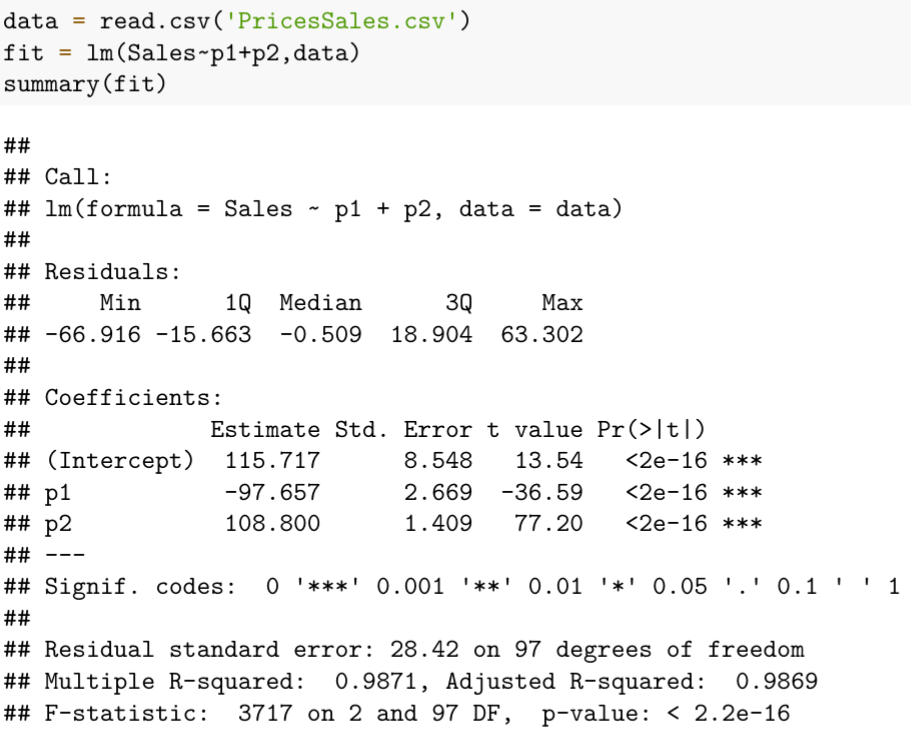
\includegraphics[scale=0.30]{figures/salesMLR1}		
%	\end{center}
%
%	
%		
%\end{frame}


%\begin{frame}
%\frametitle{Plug-in Prediction in MLR}  
%
%Suppose that by using advanced corporate espionage tactics, I discover that my competitor will charge \$10 the next quarter. After some marketing analysis I decide to charge \$8. {\color{burntorange}How much will I sell?}
%
%\vspace{-3mm}
%\sk
%Our model is: 
%$$
%\text{Sales} = \beta_0 + \beta_1 P1 + \beta_2 P2 + \epsilon
%$$
%with $\epsilon\sim N(0,\sigma^2)$\sk
%
%Our estimates are $b_0 = 115$, $b_1=-97$, $b_2=109$ and $s=28$ 
%
%which leads to
%$$
%\text{Sales} =115 + -97*P1 + 109*P2 + \epsilon 
%$$
%with $\epsilon \sim N(0,28^2)$
%
%\end{frame}
%%%%%%%%%%%%%%%%%%%%%%%%%%%%%%%%%%%%%%%%%%%%
%
%\begin{frame}
%\frametitle{Plug-in Prediction in MLR}  
%
%By plugging-in the numbers,
%
%\vspace{-3mm}
%\begin{eqnarray*}
%Sales &=&115 + -97*8 + 109*10 + \epsilon \\
%&=& 437 + \epsilon
%\end{eqnarray*}
%
%$$
%\text{Sales}|(P1 = 8, P2=10) \sim N(437,28^2)
%$$
%
%and the $95\%$ Prediction Interval is $(437 \pm 2 * 28)$
%
%{\color{burntorange}
%$$\mathbf{
%381 < \text{Sales} < 493}
%$$
%}
%\end{frame}

\begin{frame}
\frametitle{But what about the right-hand-side?}

It is also important to understand and interpret the coefficients, i.e., what is is happening on the ``right-hand-side'' of our model ... \sk

\begin{itemize}
\item {\color{burntorange}{\bf Sales}} : units sold in excess of a baseline
\item {\color{burntorange}{\bf P1}}: our price in \$ (in excess of a baseline price)
\item {\color{burntorange}{\bf P2}}: competitors price (again, over a baseline)
\end{itemize}



\end{frame}

\begin{frame}
\frametitle{But what about the right-hand-side?}


If we regress Sales on our own price, we obtain a somewhat surprising conclusion... {\color{burntorange}\bf the higher the price the more we sell!}

\vspace{2mm}
\hspace*{10mm}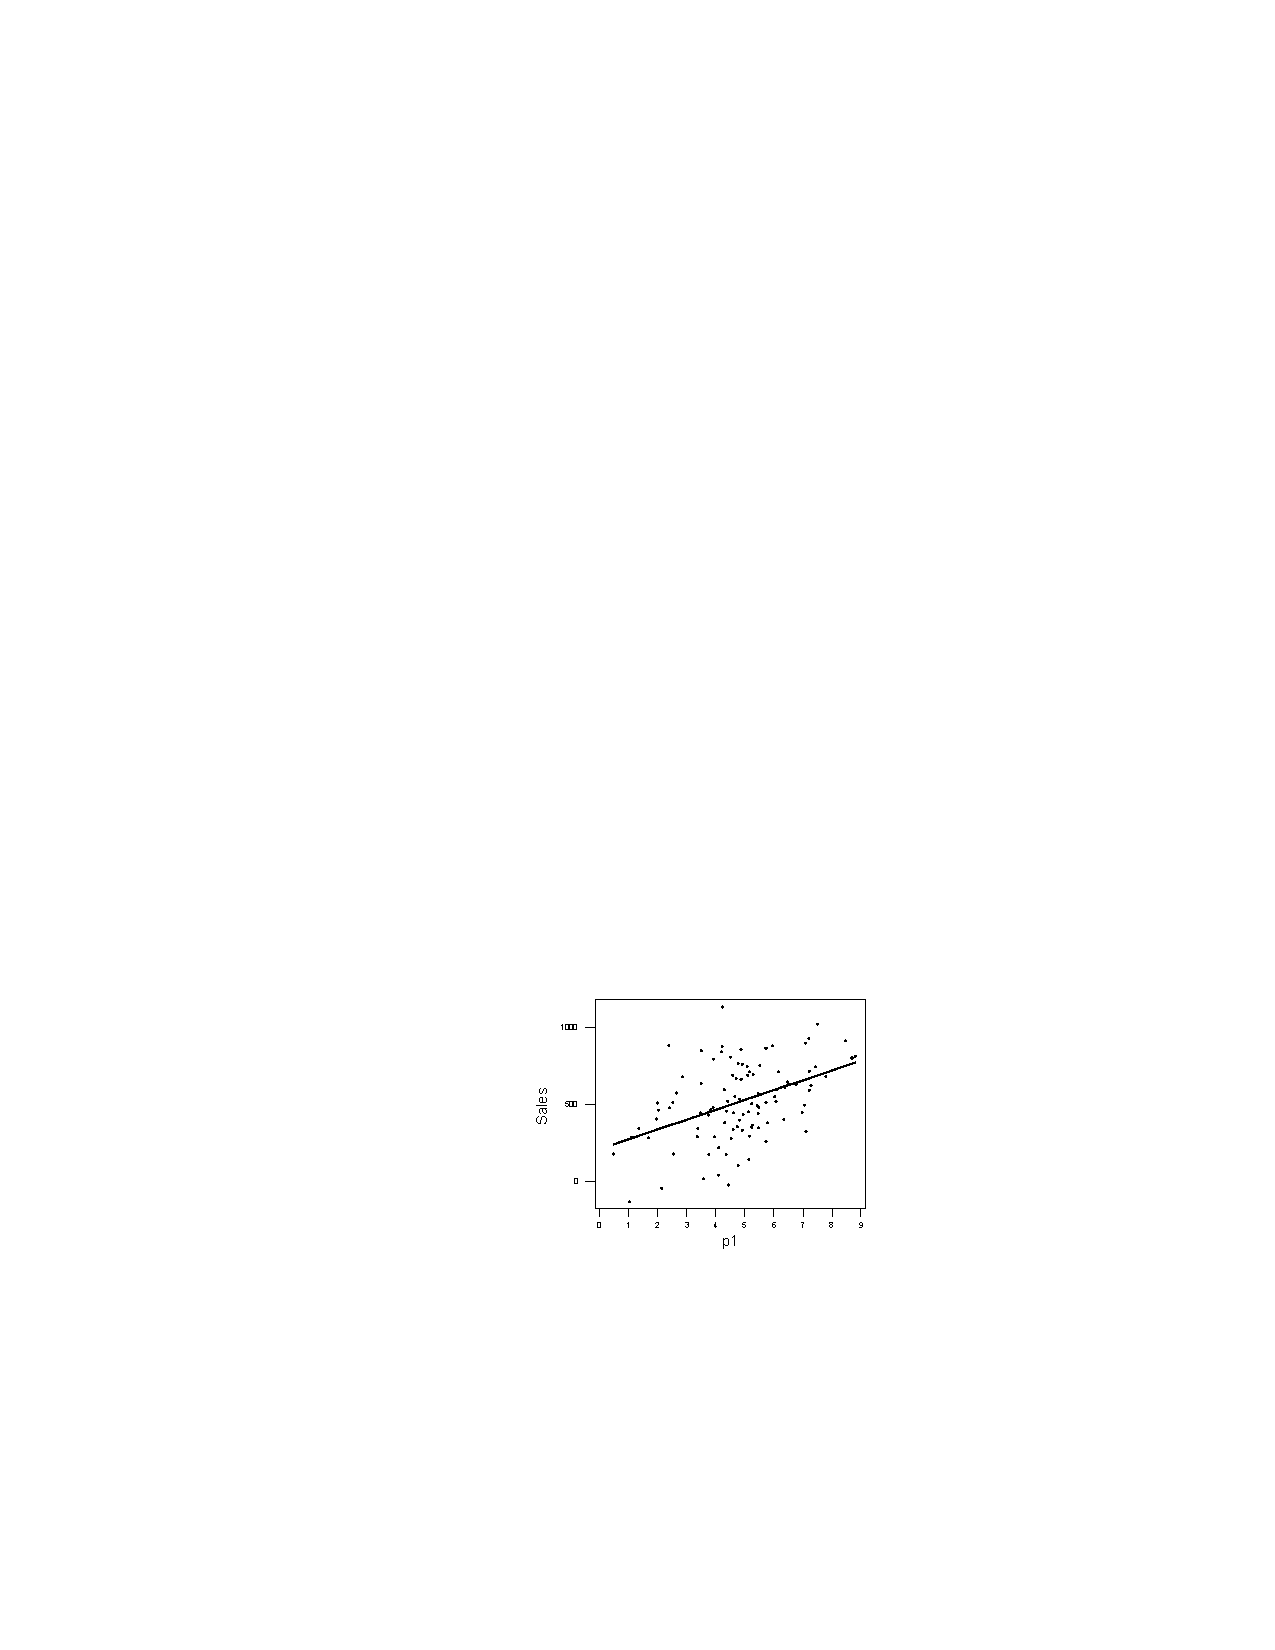
\includegraphics[width=3in]{figures/Sales1}





$\rightarrow$ It looks like we should just raise our prices, right?

\end{frame}


%%%%%%%%%%%%%%%%%%%%%%%%%%%%%%%%%%%%%%%%%%
\begin{frame}
\frametitle{Understanding multiple regression}

The regression equation for Sales on own price (P1) is: \sk
$$
Sales = 211 + 63.7 P1
$$
If now we add the competitors price to the regression we get \sk
$${\color{blue} 
	Sales = 116 - 97.7P1 + 109 P2}
$$

\sk 
Does this look better? How did it happen?
Remember: $-97.7$ is the affect on sales of a change in $P1$ {\color{burntorange}\bf with $P2$ held fixed!}

\end{frame}

%%%%%%%%%%%%%%%%%%%%%%%%%%%%%%%%%%%%%%%%%%
\begin{frame}
\frametitle{Understanding multiple regression}

How can we see what is going on? Let's compare Sales in two different observations: weeks 82 and 99. \sk

We see that an {\color{blue}increase} in $P1$, holding $P2$ {\color{blue}constant}, corresponds to a drop in Sales! 

\vspace{3mm}


\hspace*{0mm}\includegraphics[width=4.3in]{figures/Sales2}




\color{burntorange}Note the strong relationship (dependence) between $P1$ and $P2$!


\end{frame}
%%%%%%%%%%%%%%%%%%%%%%%%%%%%%%%%%%%%%%%%%%
\begin{frame}
\frametitle{Understanding multiple regression}

Let's look at a subset of points where $P1$ varies and $P2$ is held approximately constant...

\vspace{3mm}

\hspace*{-4mm}\includegraphics[width=4.5in]{figures/Sales3.png}

\color{lightblue} {\bf For a fixed level of $P2$, variation in $P1$ is negatively correlated with Sales!}

\end{frame}

%%%%%%%%%%%%%%%%%%%%%%%%%%%%%%%%%%%%%%%%%%
\begin{frame}
\frametitle{Understanding multiple regression}

\sk
Below, different colors indicate different ranges for $P2$...

\vspace{2mm}
\hspace*{-4mm}\includegraphics[width=4.5in]{figures/Sales4}
\end{frame}
%%%%%%%%%%%%%%%%%%%%%%%%%%%%%%%%%%%%%%%%%%
\begin{frame}
\frametitle{Understanding multiple regression}

\bo{\bf Summary}: \\ \sk\sk

$\dg{\rightarrow}$ A larger $P1$ is associated with larger $P2$ and the overall effect leads to bigger sales \\ \sk
$\dg{\rightarrow}$ With $P2$ held fixed, a larger $P1$ leads to lower sales \\ \sk
$\dg{\rightarrow}$ MLR does the trick and unveils the \lb{\bf correct} economic relationship between Sales and prices! \\ \sk
\end{frame}

\begin{frame}
	\frametitle{Example: Beers, height, weight, and getting drunk}

\sk
Beer data (from PRL class last year) \\
-- {\color{burntorange}{\bf nbeer}} -- number of beers before getting drunk \\
-- {\color{burntorange}{\bf height}} and {\color{burntorange}{\bf  weight}} 
	
	
\hspace*{15mm}\includegraphics[width=2.7in]{figures/beer1}
	
\lb{\bf Is number of beers related to height?}
	
\end{frame}


\begin{frame}
	\frametitle{{\tt R} output: \lb{Yes!}}
	
\hspace*{2mm}\includegraphics[width=3.8in]{figures/beersMLR1}
	
\end{frame}

\begin{frame}
	\frametitle{{\tt R} output: \bo{What about now?}}
	
	\vspace{2mm}
\hspace*{2mm}\includegraphics[width=3.8in]{figures/beersMLR2}
	
\end{frame}


\begin{frame}
\frametitle{Understanding multiple regression}


\includegraphics[width=4in]{figures/beer2}


If we regress ``beers'' only on height we see an effect.  Taller heights go with more beers. \\ \sk
However, when height goes up weight tends to go up as well... in the first regression, height was a proxy for the real \bo{\bf cause} of drinking ability. Bigger people can drink more and weight is a more accurate measure of ``bigness.''

\end{frame}

\begin{frame}
\frametitle{Understanding multiple regression}


\includegraphics[width=4in]{figures/beer2}
\sk\sk

In the multiple regression, when we consider only the variation in height that is not associated with variation in weight, we see no relationship between height and beers.


\end{frame}

\begin{frame}
	\frametitle{{\tt R} output: \lb{\normalsize Why is this a better model than height + weight?}}
	
	\vspace{2mm}
\hspace*{2mm}\includegraphics[width=3.8in]{figures/beersMLR3}
	
\end{frame}

\begin{frame}
\frametitle{Summary slide}

In general, when we see a relationship between $y$ and $x$ (or $x$'s), that relationship may be driven by variables ``lurking'' in the background which are related to your current $x$'s.

\sk
This makes it hard to reliably find {\color{lightblue}``causal''} relationships. Any correlation (association) you find could be caused by other variables in the background... 
{\color{burntorange}correlation is NOT causation}

\sk 
Any time a report says two variables are related and there's a suggestion of a {\color{lightblue}``causal''} relationship, ask yourself whether or not other variables might be the real reason for the effect. \\ \sk Multiple regression allows us to {\color{burntorange}control} for all important variables by including them into the regression. {\color{burntorange}``Once we control for weight, height and beers are NOT related''!} 
\end{frame}


\begin{frame}
\frametitle{Correlation is NOT causation}
\begin{center}
\includegraphics[width=4in]{figures/xkcd.png}
\end{center}
\end{frame}


%\begin{frame}
%\sk\sk
%	\dg{\bf Dummy variables and interactions }
%\end{frame}
%
%
%
%
%\begin{frame}[containsverbatim]
%\frametitle{Example: Detecting Sex Discrimination} 
%Imagine you are a trial lawyer and you want to file a suit against a company for \lb{salary discrimination}... you gather the following data... 
%
%\sk
%\begin{verbatim}
% Gender    Salary
%1    Male   32.0
%2  Female   39.1
%3  Female   33.2
%4  Female   30.6
%5    Male   29.0
%... ... ... 
%208	Female  30.0
%\end{verbatim}
%
%
%\end{frame}
%%%%%%%%%%%%%%%%%%%%%%%%%%%%%%%%%%%%%%%%%%%
%
%\begin{frame}
%\frametitle{Detecting sex discrimination}
%You want to relate salary ($Y$) to gender ($X$)...  how can we do that?
%
%\skoo
%
%Gender is an example of a {\bo{\bf categorical variable}}. The gender variable separates our data into 2 \lb{groups} or \lb{categories}. \\ \sk 
%
%The question we want to answer is: {\it ``how is your salary related to which group you belong to...?''}  
%
%\skoo \pause
%
%\dg{Could we think about additional examples of categories potentially associated with salary?} \vspace{2mm} 
%\begin{itemize}
%\item UT education vs. not
%\item foreign or domestic born citizen
%\item quarterback vs. wide receiver 
%\end{itemize}
%\end{frame}
%
%%%%%%%%%%%%%%%%%%%%%%%%%%%%%%%%%%%%%%%%%%%
%
%\begin{frame}[containsverbatim]
%\frametitle{Detecting sex discrimination}
%
%
%We can use \bo{regression} to answer these questions, but first we need to recode the categorical variable into a {\bo{\bf dummy variable}}:
%
%
%\begin{verbatim}
% Gender    Salary  Sex
%1     Male  32.00   1
%2   Female  39.10   0
%3   Female  33.20   0
%4   Female  30.60   0
%5     Male  29.00   1
%... ... ... 
%208  Female  30.00  0
%\end{verbatim}	
%
%
%{\color{red} Note:} \\ \vspace{2mm}
%
%{\small
%This can be done implicitly in {\tt R} by, {\tt Sex = factor(Gender)}. \dg{This tells {\tt R} that Sex is a variable separated into its unique levels, in this case just 2!}  }
%
%
%
%\end{frame}
%
%
%%%%%%%%%%%%%%%%%%%%%%%%%%%%%%%%%%%%%%%%%%%
%
%\begin{frame}
%\frametitle{Detecting sex discrimination}
%Now you can present the following model in court:
%
%$$
%\text{Salary}_i = \beta_0 + \beta_1\text{Sex}_i + \epsilon_i
%$$
%
%\sk
%{\color{burntorange} How do you interpret $\beta_1$?  What is your predicted salary for males and females?} \pause
%\begin{eqnarray*}
%E[\text{Salary} | \text{Sex} = 0] &=& \beta_0 \\
%E[\text{Salary} | \text{Sex} = 1] &=& \beta_0 + \beta_1
%\end{eqnarray*}
%
%\sk
%$\beta_1$ is the male-female difference!
%
%\end{frame}
%%%%%%%%%%%%%%%%%%%%%%%%%%%%%%%%%%%%%%%%%%
%\begin{frame}
%\frametitle{Detecting sex discrimination}
%
%\vspace{1mm}
%\hspace*{30mm}$\text{Salary}_i = \beta_0 + \beta_1\text{Sex}_i + \epsilon_i$
%\vspace{3mm}
%
%
%
%\hspace*{10mm}\includegraphics[width=3.1in]{figures/sexMLR1}
%
%\vspace{3mm}
%
%
%{\small
%{\color{burntorange}$\hat{\beta}_1 = b_1 = 8.29$... on average, a male makes approximately \$8,300 more than a female in this firm.} }
%
%\end{frame}
%
%\begin{frame}
%	\frametitle{We've seen this before!}
%	
%	{What is the below code demonstrating?} \sk
%	
%\hspace*{8mm}\includegraphics[width=3.5in]{figures/sexMLR2}	
%\end{frame}
%
%\begin{frame}
%\frametitle{Detecting sex discrimination}
% {\color{burntorange} How can the defense attorney try to counteract the plaintiff's argument?}
%
%\skoo
%
%Perhaps, the observed difference in salaries is related to other variables in the background and {\color{lightblue}NOT} to gender discrimination...
%
%\skoo
%Obviously, there are many other factors which we can legitimately use in determining salaries:
%\bi
%\item education
%\item job productivity
%\item experience
%\ib
%
%\sko
%{\color{lightblue}How can we use regression to incorporate additional information?}
%
%\end{frame}
%
%
%\begin{frame}
%\frametitle{Detecting sex discrimination}
%Let's add a measure of experience...
%
%\sk
%$$
%\text{Salary}_i = \beta_0 + \beta_1\text{Sex}_i + \beta_2\text{Exp}_i + \epsilon_i
%$$
%
%\sk
%
%{\color{burntorange} What does that mean?  Write out the model for each gender separately:}
%\begin{eqnarray*}
%E[\text{Salary} | \text{Sex} = 0, \text{Exp}] &=& \beta_0 + \beta_2 \text{Exp} \\
%E[\text{Salary} | \text{Sex} = 1, \text{Exp}] &=& (\beta_0 + \beta_1) + \beta_2 \text{Exp}
%\end{eqnarray*}
%
%
%\end{frame}
%
%%%%%%%%%%%%%%%%%%%%%%%%%%%%%%%
%\begin{frame}[containsverbatim]
%\frametitle{Detecting sex discrimination}
%
%Here is our \lb{data} with this \dg{additional variable}:
%
%\sk
%\begin{verbatim}
%    Exp   Gender   Salary  Sex
%1        3   Male  32.00   1
%2       14 Female  39.10   0
%3       12 Female  33.20   0
%4        8 Female  30.60   0
%5        3   Male  29.00   1
%... ... ... 
%208      33 Female  30.00  0
%\end{verbatim}
%\end{frame}
%
%\begin{frame}
%\frametitle{Detecting sex discrimination}
%
%\sko
%$\text{Salary}_i = \beta_0 + \beta_1\text{Sex}_i + \beta_2 \text{Exp} + \epsilon_i$
%
%\sko
%\hspace*{10mm}\includegraphics[width=3.5in]{figures/sexMLR3}
%
%\sko
%$
%\lb{\rightarrow} \hspace{3mm} \text{Salary}_i = 27 + 8 \text{Sex}_i  +0.98 \text{Exp}_i + \epsilon_i
%$
%
%
%\vspace{1mm}
%{\color{burntorange} \bf Is this good or bad news for the defense?}
%\end{frame}
%
%
%\begin{frame}
%\frametitle{Detecting sex discrimination}
%
%\sko
%$\text{Salary}_i = \left\{ \begin{array}{l}
%{\color{red}27 + 0.98 \text{Exp}_i + \epsilon_i \quad \mbox{females}} \\
%{\color{blue}35 + 0.98 \text{Exp}_i + \epsilon_i  \quad \mbox{males}}
% \end{array}
% \right.$
%
%
%\vspace{-7mm}
%\hspace*{10mm}\includegraphics[width=3.2in]{figures/SalaryExp.pdf}
%
%\end{frame}
%
%
%\begin{frame}
%\frametitle{More than two categories}
%
%\sk
%We can use \bo{dummy variables} in situations in which there are more than two categories. Dummy variables are needed for each category except one, designated as the ``\underline{base}'' category.
%
%\sk\sk
%
%		{\color{lightblue}Why? {\bf Remember that the numerical value of each category has no quantitative meaning!}}
%
%\sk
%
%\end{frame}
%
%
%\begin{frame}[containsverbatim]
%\frametitle{House prices revisted}
%We want to evaluate the difference in house prices in a couple of different neighborhoods. 
%
%
%\begin{verbatim}
%   Nbhd SqFt  Price
%1     2 1.79  114.3
%2     2 2.03  114.2
%3     2 1.74  114.8
%4     2 1.98   94.7
%5     2 2.13  119.8
%6     1 1.78  114.6
%7     3 1.83  151.6
%8     3 2.16  150.7
%... ... ... ... 
%
%\end{verbatim}
%
%\end{frame}
%%%%%%%%%%%%%%%%%%%%%%%%%%%%%%%%%%%%%%
%\begin{frame}[containsverbatim]
%\frametitle{House prices revisted}
%Let's create the {\color{lightblue}dummy variables} dn1, dn2 and dn3... 
% \begin{verbatim}
%   Nbhd  SqFt  Price  dn1 dn2 dn3
%1      2 1.79 114.3   0   1   0
%2      2 2.03 114.2   0   1   0
%3      2 1.74 114.8   0   1   0
%4      2 1.98  94.7   0   1   0
%5      2 2.13 119.8   0   1   0
%6      1 1.78 114.6   1   0   0
%7      3 1.83 151.6   0   0   1
%8      3 2.16 150.7   0   0   1
%... ... ... 
%\end{verbatim}
%\end{frame}
%%%%%%%%%%%%%%%%%%%%%%%%%%%%%%%%%%%%%
%\begin{frame}
%\frametitle{House prices revisted}
%$$
%\text{Price}_i = \beta_0 + \beta_1 \text{dn1}_i + \beta_2 \text{dn2}_i + \beta_3 \text{SqFt}_i + \epsilon_i
%$$
%
%\begin{eqnarray*}
%E[\text{Price}|\text{dn1}=1,\text{SqFt}] &=& \beta_0 + \beta_1 + \beta_3 \text{SqFt} \quad \mbox{(\bo{Nbhd 1})} \\ \pause 
%E[\text{Price}|\text{dn2}=1,\text{SqFt}] &=& \beta_0 + \beta_2 + \beta_3 \text{SqFt} \quad \mbox{(\bo{Nbhd 2})} \\ \pause 
%E[\text{Price}|\text{dn1}=0,\text{dn2}=0,\text{SqFt}] &=& \beta_0 +\beta_3 \text{SqFt} \quad \quad \quad \ \mbox{(\bo{Nbhd 3})} \\
%\end{eqnarray*}
%\end{frame}
%%%%%%%%%%%%%%%%%%%%%%
%
%
%\begin{frame}
%	\frametitle{Model output}
%	
%\sko	
%\hspace*{8mm}\includegraphics[width=3.3in]{figures/houseMLR1}	
%
%\sko
%$
%\text{Price} = 62.78 -41.54 * \text{dn1} -30.97 * \text{dn2} + 46.39 * \text{SqFt} + \epsilon
%$
%
%\end{frame}
%
%\begin{frame}
%\frametitle{What do these models look like?}
%
%\vspace{-2.3cm}
%\begin{center}
%\includegraphics[width=3.7in]{figures/MidCityPlot1}
%\end{center}
%\end{frame}
%%%%%%%%%%%%%%%%%%%%%%%%%%%%%%%%%%%%%
%
%%%%%%%%%%%%%%%%%%%%%%%%%%%%%%%%%%%%%
%\begin{frame}
%\frametitle{Model output only with ``SqFt''}
%
%\sko	
%\hspace*{8mm}\includegraphics[width=3.3in]{figures/houseMLR2}	
%
%\sko
%$
%\text{Price} = -10.09 + 70.23 * \text{SqFt} + \epsilon
%$
%\end{frame}
%%%%%%%%%%%%%%%%%%%%%%%%%%%%%%%%%%%%%
%
%
%%%%%%%%%%%%%%%%%%%%%%%%%%%%%%%%%%%%%
%\begin{frame}
%\frametitle{What do these models look like?}
%\vspace{-2.4cm}
%\begin{center}
%\includegraphics[width=3.75in]{figures/MidCityPlot2}
%\end{center}
%\end{frame}
%
%\begin{frame}
%\frametitle{Back to the sex discrimination case}
%\vspace{-1.2cm}
%\begin{center}
%\includegraphics[width=3.1in]{figures/SalaryExp.pdf}
%\end{center}
%\vspace{-0.5cm}
%{\color{lightblue}\bf Does it look like the effect of experience on salary is the same for males and females?}
%\end{frame}
%
%%%%%%%%%%%%%%%%%%%%%%%%%%%%%%%%%%%%%
%\begin{frame}
%\frametitle{Back to the sex discrimination case}
%
%\sko
%Could we try to expand our analysis by allowing a different slope for each group?
%\skoo
%
%Yes... Consider the following model:
%$$
%\text{Salary}_i = \beta_0 + \beta_1 \text{Exp}_i + \beta_2 \text{Sex}_i + \beta_3 \text{Exp}_i \times \text{Sex}_i + \epsilon_i
%$$
%
%\skoo
%{\color{red}For Females:
%$$
%\text{Salary}_i = \beta_0 + \beta_1 \text{Exp}_i  + \epsilon_i
%$$
%}
%{\color{blue}For Males:
%$$
%\text{Salary}_i = (\beta_0 + \beta_2) + (\beta_1+\beta_3) \text{Exp}_i  + \epsilon_i
%$$
%}
%
%\bo{\bf How are these models different from each other?}
%
%\end{frame}
%
%
%\begin{frame}[containsverbatim]
%\frametitle{Sex discrimination case}
%
%We are just creating a \lb{new variable}!
%
%\sk
%\begin{verbatim}
%    Exp   Gender   Salary  Sex  Exp*Sex
%1        3   Male  32.00   1      3
%2       14 Female  39.10   0      0
%3       12 Female  33.20   0      0
%4        8 Female  30.60   0      0
%5        3   Male  29.00   1      3
%... ... ... 
%208     33 Female  30.00   0      0
%\end{verbatim}
%
%
%\end{frame}
%
%\begin{frame}
%\frametitle{Sex discrimination case}
%
%
%\sko	
%\hspace*{8mm}\includegraphics[width=3.3in]{figures/sexMLR4}	
%
%\sko
%$
%\text{Salary} = 34 - 4*\text{Sex}+ 0.28*\text{Exp} + 1.24*\text{Exp$*$Sex} + \epsilon
%$
%\end{frame}
%
%
%\begin{frame}
%\frametitle{Sex discrimination case}
%\vspace{-1cm}
%\begin{center}
%\includegraphics[width=3.2in]{figures/SalaryExp_INT.pdf}
%\end{center}
%\vspace{-.5cm}
%{\color{burntorange}\bf Is this good or bad news for the plaintiff?}
%
%\end{frame}
%
%\begin{frame}
%\frametitle{Variable interaction}
%
%The effect of experience on salary is different for males and females... in general, when the effect of the variable $X_1$ onto $Y$ depends on another variable  $X_2$ we say that $X_1$ and $X_2$ {\color{burntorange}\bf interact} with each other.
%  
%\sk
%We can extend this notion by the inclusion of multiplicative 
%effects through interaction terms.
%
%
%$$
%Y= \beta_0 + \beta_1 X_{1} + \beta_2 X_{2} + \beta_3(X_{1} X_{2}) + \epsilon
%$$
%
%$$
%\lb{
%\frac{\partial E[Y | X_1,X_2]}{\partial X_1} = \beta_1 + \beta_3 X_{2}}
%$$
%
%\end{frame}
%
%\begin{frame}
%	\frametitle{More topics in regression}
%	
%	\begin{itemize}
%		\item How do you model $Y$ when it is \lb{\bf binary}? \bo{Logistic regression ...} \sko
%		\item How to select the \lb{\bf best} model? \bo{Hand pick covariates, forward or backward stepwise selection, LASSO, ...} \sko
%		\item How to get \lb{\bf causal estimates} from regression?  \bo{Regression on binary variable, Regression on treatment and covariates (confounding), ``Regression discontinuity''...} \sko
%		\item My causal estimates are usually differences in group averages, what about \lb{\bf individualized causal effects}? \bo{Heterogenous treatment effects, ensemble learning and BART ...}
%	\end{itemize}
%	
%	
%\end{frame}
%
%
%\begin{frame}
%	\frametitle{More topics in regression}
%	
%	\begin{itemize}
%		\item How to get \lb{\bf causal estimates} from regression?  \bo{Regression on binary variable, Regression on treatment and covariates (confounding), ... \vspace{3mm}\\ {\bf``Regression discontinuity''} \vspace{1mm}\\ {\bf``DiD (again!)''}} \sko
%	\end{itemize}
%	
%	
%	\skooo
%	Let's go to some code! {\tt DiD.R} and {\tt RD.R}
%	
%	
%	
%\end{frame}




\end{document} 